\documentclass[twoside]{book}

% Packages required by doxygen
\usepackage{fixltx2e}
\usepackage{calc}
\usepackage{doxygen}
\usepackage[export]{adjustbox} % also loads graphicx
\usepackage{graphicx}
\usepackage[utf8]{inputenc}
\usepackage{makeidx}
\usepackage{multicol}
\usepackage{multirow}
\PassOptionsToPackage{warn}{textcomp}
\usepackage{textcomp}
\usepackage[nointegrals]{wasysym}
\usepackage[table]{xcolor}

% Font selection
\usepackage[T1]{fontenc}
\usepackage[scaled=.90]{helvet}
\usepackage{courier}
\usepackage{amssymb}
\usepackage{sectsty}
\renewcommand{\familydefault}{\sfdefault}
\allsectionsfont{%
  \fontseries{bc}\selectfont%
  \color{darkgray}%
}
\renewcommand{\DoxyLabelFont}{%
  \fontseries{bc}\selectfont%
  \color{darkgray}%
}
\newcommand{\+}{\discretionary{\mbox{\scriptsize$\hookleftarrow$}}{}{}}

% Page & text layout
\usepackage{geometry}
\geometry{%
  a4paper,%
  top=2.5cm,%
  bottom=2.5cm,%
  left=2.5cm,%
  right=2.5cm%
}
\tolerance=750
\hfuzz=15pt
\hbadness=750
\setlength{\emergencystretch}{15pt}
\setlength{\parindent}{0cm}
\setlength{\parskip}{3ex plus 2ex minus 2ex}
\makeatletter
\renewcommand{\paragraph}{%
  \@startsection{paragraph}{4}{0ex}{-1.0ex}{1.0ex}{%
    \normalfont\normalsize\bfseries\SS@parafont%
  }%
}
\renewcommand{\subparagraph}{%
  \@startsection{subparagraph}{5}{0ex}{-1.0ex}{1.0ex}{%
    \normalfont\normalsize\bfseries\SS@subparafont%
  }%
}
\makeatother

% Headers & footers
\usepackage{fancyhdr}
\pagestyle{fancyplain}
\fancyhead[LE]{\fancyplain{}{\bfseries\thepage}}
\fancyhead[CE]{\fancyplain{}{}}
\fancyhead[RE]{\fancyplain{}{\bfseries\leftmark}}
\fancyhead[LO]{\fancyplain{}{\bfseries\rightmark}}
\fancyhead[CO]{\fancyplain{}{}}
\fancyhead[RO]{\fancyplain{}{\bfseries\thepage}}
\fancyfoot[LE]{\fancyplain{}{}}
\fancyfoot[CE]{\fancyplain{}{}}
\fancyfoot[RE]{\fancyplain{}{\bfseries\scriptsize Generated by Doxygen }}
\fancyfoot[LO]{\fancyplain{}{\bfseries\scriptsize Generated by Doxygen }}
\fancyfoot[CO]{\fancyplain{}{}}
\fancyfoot[RO]{\fancyplain{}{}}
\renewcommand{\footrulewidth}{0.4pt}
\renewcommand{\chaptermark}[1]{%
  \markboth{#1}{}%
}
\renewcommand{\sectionmark}[1]{%
  \markright{\thesection\ #1}%
}

% Indices & bibliography
\usepackage{natbib}
\usepackage[titles]{tocloft}
\setcounter{tocdepth}{3}
\setcounter{secnumdepth}{5}
\makeindex

% Hyperlinks (required, but should be loaded last)
\usepackage{ifpdf}
\ifpdf
  \usepackage[pdftex,pagebackref=true]{hyperref}
\else
  \usepackage[ps2pdf,pagebackref=true]{hyperref}
\fi
\hypersetup{%
  colorlinks=true,%
  linkcolor=blue,%
  citecolor=blue,%
  unicode%
}

% Custom commands
\newcommand{\clearemptydoublepage}{%
  \newpage{\pagestyle{empty}\cleardoublepage}%
}

\usepackage{caption}
\captionsetup{labelsep=space,justification=centering,font={bf},singlelinecheck=off,skip=4pt,position=top}

%===== C O N T E N T S =====

\begin{document}

% Titlepage & ToC
\hypersetup{pageanchor=false,
             bookmarksnumbered=true,
             pdfencoding=unicode
            }
\pagenumbering{alph}
\begin{titlepage}
\vspace*{7cm}
\begin{center}%
{\Large My Project }\\
\vspace*{1cm}
{\large Generated by Doxygen 1.8.13}\\
\end{center}
\end{titlepage}
\clearemptydoublepage
\pagenumbering{roman}
\tableofcontents
\clearemptydoublepage
\pagenumbering{arabic}
\hypersetup{pageanchor=true}

%--- Begin generated contents ---
\chapter{Hierarchical Index}
\section{Class Hierarchy}
This inheritance list is sorted roughly, but not completely, alphabetically\+:\begin{DoxyCompactList}
\item Bundle\+Activator\begin{DoxyCompactList}
\item \contentsline{section}{com.\+fware.\+cspdt.\+cspm.\+Csp\+M\+Plugin}{\pageref{classcom_1_1fware_1_1cspdt_1_1cspm_1_1_csp_m_plugin}}{}
\end{DoxyCompactList}
\end{DoxyCompactList}

\chapter{Class Index}
\section{Class List}
Here are the classes, structs, unions and interfaces with brief descriptions\+:\begin{DoxyCompactList}
\item\contentsline{section}{\hyperlink{classcom_1_1fware_1_1cspdt_1_1cspm_1_1core_1_1parser_1_1_csp_m_analyser_exception}{com.\+fware.\+cspdt.\+cspm.\+core.\+parser.\+Csp\+M\+Analyser\+Exception} \\*Excecao disparada quando a analise lexica de um no na ast falha }{\pageref{classcom_1_1fware_1_1cspdt_1_1cspm_1_1core_1_1parser_1_1_csp_m_analyser_exception}}{}
\item\contentsline{section}{\hyperlink{classcom_1_1fware_1_1cspdt_1_1cspm_1_1core_1_1_csp_m_core_plugin}{com.\+fware.\+cspdt.\+cspm.\+core.\+Csp\+M\+Core\+Plugin} \\*Classe principal do plug-\/in }{\pageref{classcom_1_1fware_1_1cspdt_1_1cspm_1_1core_1_1_csp_m_core_plugin}}{}
\item\contentsline{section}{\hyperlink{classcom_1_1fware_1_1cspdt_1_1cspm_1_1core_1_1model_1_1_csp_m_model}{com.\+fware.\+cspdt.\+cspm.\+core.\+model.\+Csp\+M\+Model} \\*Essa classe contera os dados de analise do codigo }{\pageref{classcom_1_1fware_1_1cspdt_1_1cspm_1_1core_1_1model_1_1_csp_m_model}}{}
\item\contentsline{section}{\hyperlink{classcom_1_1fware_1_1cspdt_1_1cspm_1_1core_1_1parser_1_1_csp_m_parser}{com.\+fware.\+cspdt.\+cspm.\+core.\+parser.\+Csp\+M\+Parser} \\*Uma classe para usar a analise lexica e sintatica do codigo C\+SP }{\pageref{classcom_1_1fware_1_1cspdt_1_1cspm_1_1core_1_1parser_1_1_csp_m_parser}}{}
\item\contentsline{section}{\hyperlink{classcom_1_1fware_1_1cspdt_1_1cspm_1_1core_1_1parser_1_1_csp_m_parser_exception}{com.\+fware.\+cspdt.\+cspm.\+core.\+parser.\+Csp\+M\+Parser\+Exception} \\*Excecao disparada quando a analise sintatica de um no na ast falha }{\pageref{classcom_1_1fware_1_1cspdt_1_1cspm_1_1core_1_1parser_1_1_csp_m_parser_exception}}{}
\item\contentsline{section}{\hyperlink{classcom_1_1fware_1_1cspdt_1_1cspm_1_1core_1_1model_1_1_csp_m_ref}{com.\+fware.\+cspdt.\+cspm.\+core.\+model.\+Csp\+M\+Ref} \\*Essa classe representa uma referencia dentro do documento C\+SP }{\pageref{classcom_1_1fware_1_1cspdt_1_1cspm_1_1core_1_1model_1_1_csp_m_ref}}{}
\item\contentsline{section}{\hyperlink{classcom_1_1fware_1_1cspdt_1_1cspm_1_1core_1_1model_1_1_token_extractor}{com.\+fware.\+cspdt.\+cspm.\+core.\+model.\+Token\+Extractor} \\*Classe que extrai tokens da ast }{\pageref{classcom_1_1fware_1_1cspdt_1_1cspm_1_1core_1_1model_1_1_token_extractor}}{}
\end{DoxyCompactList}

\chapter{Class Documentation}
\hypertarget{classcom_1_1fware_1_1cspdt_1_1cspm_1_1editor_1_1outline_1_1_csp_m_ast_tree_node_generator}{}\section{com.\+fware.\+cspdt.\+cspm.\+editor.\+outline.\+Csp\+M\+Ast\+Tree\+Node\+Generator Class Reference}
\label{classcom_1_1fware_1_1cspdt_1_1cspm_1_1editor_1_1outline_1_1_csp_m_ast_tree_node_generator}\index{com.\+fware.\+cspdt.\+cspm.\+editor.\+outline.\+Csp\+M\+Ast\+Tree\+Node\+Generator@{com.\+fware.\+cspdt.\+cspm.\+editor.\+outline.\+Csp\+M\+Ast\+Tree\+Node\+Generator}}


\hyperlink{classcom_1_1fware_1_1cspdt_1_1cspm_1_1editor_1_1outline_1_1_csp_m_ast_tree_node_generator}{Csp\+M\+Ast\+Tree\+Node\+Generator}.  


Inheritance diagram for com.\+fware.\+cspdt.\+cspm.\+editor.\+outline.\+Csp\+M\+Ast\+Tree\+Node\+Generator\+:\begin{figure}[H]
\begin{center}
\leavevmode
\includegraphics[height=2.000000cm]{classcom_1_1fware_1_1cspdt_1_1cspm_1_1editor_1_1outline_1_1_csp_m_ast_tree_node_generator}
\end{center}
\end{figure}
\subsection*{Public Member Functions}
\begin{DoxyCompactItemize}
\item 
\mbox{\Hypertarget{classcom_1_1fware_1_1cspdt_1_1cspm_1_1editor_1_1outline_1_1_csp_m_ast_tree_node_generator_a32b7e0291ecc55febae62c17f2d6d934}\label{classcom_1_1fware_1_1cspdt_1_1cspm_1_1editor_1_1outline_1_1_csp_m_ast_tree_node_generator_a32b7e0291ecc55febae62c17f2d6d934}} 
{\bfseries Csp\+M\+Ast\+Tree\+Node\+Generator} (I\+Document document, boolean detailed)
\item 
\mbox{\Hypertarget{classcom_1_1fware_1_1cspdt_1_1cspm_1_1editor_1_1outline_1_1_csp_m_ast_tree_node_generator_a2a761c958cb51e77c2753d6558b276c7}\label{classcom_1_1fware_1_1cspdt_1_1cspm_1_1editor_1_1outline_1_1_csp_m_ast_tree_node_generator_a2a761c958cb51e77c2753d6558b276c7}} 
\hyperlink{classcom_1_1fware_1_1cspdt_1_1cspm_1_1editor_1_1outline_1_1_csp_m_outline_tree_node}{Csp\+M\+Outline\+Tree\+Node} {\bfseries get\+Root\+Node} ()
\item 
\mbox{\Hypertarget{classcom_1_1fware_1_1cspdt_1_1cspm_1_1editor_1_1outline_1_1_csp_m_ast_tree_node_generator_ab24faf27b17e8d97538dd1fdce191b61}\label{classcom_1_1fware_1_1cspdt_1_1cspm_1_1editor_1_1outline_1_1_csp_m_ast_tree_node_generator_ab24faf27b17e8d97538dd1fdce191b61}} 
void {\bfseries in\+Start} (Start node)
\item 
\mbox{\Hypertarget{classcom_1_1fware_1_1cspdt_1_1cspm_1_1editor_1_1outline_1_1_csp_m_ast_tree_node_generator_a8ff5d0f32c79a5ad0d716e1781b8a453}\label{classcom_1_1fware_1_1cspdt_1_1cspm_1_1editor_1_1outline_1_1_csp_m_ast_tree_node_generator_a8ff5d0f32c79a5ad0d716e1781b8a453}} 
void {\bfseries out\+Start} (Start node)
\item 
\mbox{\Hypertarget{classcom_1_1fware_1_1cspdt_1_1cspm_1_1editor_1_1outline_1_1_csp_m_ast_tree_node_generator_aaf21dace45d16d2acf48c16274515090}\label{classcom_1_1fware_1_1cspdt_1_1cspm_1_1editor_1_1outline_1_1_csp_m_ast_tree_node_generator_aaf21dace45d16d2acf48c16274515090}} 
void {\bfseries in\+A\+Csp\+Specification} (A\+Csp\+Specification node)
\item 
\mbox{\Hypertarget{classcom_1_1fware_1_1cspdt_1_1cspm_1_1editor_1_1outline_1_1_csp_m_ast_tree_node_generator_a82a56235da58604bec83be57e52c0fc7}\label{classcom_1_1fware_1_1cspdt_1_1cspm_1_1editor_1_1outline_1_1_csp_m_ast_tree_node_generator_a82a56235da58604bec83be57e52c0fc7}} 
void {\bfseries out\+A\+Csp\+Specification} (A\+Csp\+Specification node)
\item 
\mbox{\Hypertarget{classcom_1_1fware_1_1cspdt_1_1cspm_1_1editor_1_1outline_1_1_csp_m_ast_tree_node_generator_a65de4e86306073573bfeff9525a76dea}\label{classcom_1_1fware_1_1cspdt_1_1cspm_1_1editor_1_1outline_1_1_csp_m_ast_tree_node_generator_a65de4e86306073573bfeff9525a76dea}} 
void {\bfseries in\+A\+Csp\+Definition\+Paragraph} (A\+Csp\+Definition\+Paragraph node)
\item 
\mbox{\Hypertarget{classcom_1_1fware_1_1cspdt_1_1cspm_1_1editor_1_1outline_1_1_csp_m_ast_tree_node_generator_a6f99176c607677e4e0793aa5c64dda88}\label{classcom_1_1fware_1_1cspdt_1_1cspm_1_1editor_1_1outline_1_1_csp_m_ast_tree_node_generator_a6f99176c607677e4e0793aa5c64dda88}} 
void {\bfseries out\+A\+Csp\+Definition\+Paragraph} (A\+Csp\+Definition\+Paragraph node)
\item 
\mbox{\Hypertarget{classcom_1_1fware_1_1cspdt_1_1cspm_1_1editor_1_1outline_1_1_csp_m_ast_tree_node_generator_a85a4b873012f6f43fbdb227320d6a218}\label{classcom_1_1fware_1_1cspdt_1_1cspm_1_1editor_1_1outline_1_1_csp_m_ast_tree_node_generator_a85a4b873012f6f43fbdb227320d6a218}} 
void {\bfseries case\+A\+Csp\+Comment\+Paragraph} (A\+Csp\+Comment\+Paragraph node)
\item 
\mbox{\Hypertarget{classcom_1_1fware_1_1cspdt_1_1cspm_1_1editor_1_1outline_1_1_csp_m_ast_tree_node_generator_ab879c64711f94f85ac358e7539909037}\label{classcom_1_1fware_1_1cspdt_1_1cspm_1_1editor_1_1outline_1_1_csp_m_ast_tree_node_generator_ab879c64711f94f85ac358e7539909037}} 
void {\bfseries case\+A\+Csp\+Definition\+Paragraph} (A\+Csp\+Definition\+Paragraph node)
\item 
\mbox{\Hypertarget{classcom_1_1fware_1_1cspdt_1_1cspm_1_1editor_1_1outline_1_1_csp_m_ast_tree_node_generator_a46c78b2e563ff614ac28fcc16685bd0a}\label{classcom_1_1fware_1_1cspdt_1_1cspm_1_1editor_1_1outline_1_1_csp_m_ast_tree_node_generator_a46c78b2e563ff614ac28fcc16685bd0a}} 
void {\bfseries case\+A\+Csp\+Function\+Definition} (A\+Csp\+Function\+Definition node)
\item 
\mbox{\Hypertarget{classcom_1_1fware_1_1cspdt_1_1cspm_1_1editor_1_1outline_1_1_csp_m_ast_tree_node_generator_a67c619b3c9a974bd86fbf2a3c587ed8b}\label{classcom_1_1fware_1_1cspdt_1_1cspm_1_1editor_1_1outline_1_1_csp_m_ast_tree_node_generator_a67c619b3c9a974bd86fbf2a3c587ed8b}} 
void {\bfseries case\+A\+Csp\+Constant\+Definition} (A\+Csp\+Constant\+Definition node)
\item 
\mbox{\Hypertarget{classcom_1_1fware_1_1cspdt_1_1cspm_1_1editor_1_1outline_1_1_csp_m_ast_tree_node_generator_a3e84459dc5c77e30726914ab7cfe106f}\label{classcom_1_1fware_1_1cspdt_1_1cspm_1_1editor_1_1outline_1_1_csp_m_ast_tree_node_generator_a3e84459dc5c77e30726914ab7cfe106f}} 
void {\bfseries case\+A\+Csp\+Datatype\+Definition} (A\+Csp\+Datatype\+Definition node)
\item 
\mbox{\Hypertarget{classcom_1_1fware_1_1cspdt_1_1cspm_1_1editor_1_1outline_1_1_csp_m_ast_tree_node_generator_af295febf9cf4f424494a1f718a2b3ab2}\label{classcom_1_1fware_1_1cspdt_1_1cspm_1_1editor_1_1outline_1_1_csp_m_ast_tree_node_generator_af295febf9cf4f424494a1f718a2b3ab2}} 
void {\bfseries case\+A\+Csp\+Subtype\+Definition} (A\+Csp\+Subtype\+Definition node)
\item 
\mbox{\Hypertarget{classcom_1_1fware_1_1cspdt_1_1cspm_1_1editor_1_1outline_1_1_csp_m_ast_tree_node_generator_a7f98db9afff59f70ee2bbda5304fee5f}\label{classcom_1_1fware_1_1cspdt_1_1cspm_1_1editor_1_1outline_1_1_csp_m_ast_tree_node_generator_a7f98db9afff59f70ee2bbda5304fee5f}} 
void {\bfseries case\+A\+Csp\+Nametype\+Definition} (A\+Csp\+Nametype\+Definition node)
\item 
\mbox{\Hypertarget{classcom_1_1fware_1_1cspdt_1_1cspm_1_1editor_1_1outline_1_1_csp_m_ast_tree_node_generator_a4ea8da576fda7121d212a46c416fe064}\label{classcom_1_1fware_1_1cspdt_1_1cspm_1_1editor_1_1outline_1_1_csp_m_ast_tree_node_generator_a4ea8da576fda7121d212a46c416fe064}} 
void {\bfseries case\+A\+Csp\+Process\+Definition} (A\+Csp\+Process\+Definition node)
\item 
\mbox{\Hypertarget{classcom_1_1fware_1_1cspdt_1_1cspm_1_1editor_1_1outline_1_1_csp_m_ast_tree_node_generator_aaba17612415cc210858584129d4b4aab}\label{classcom_1_1fware_1_1cspdt_1_1cspm_1_1editor_1_1outline_1_1_csp_m_ast_tree_node_generator_aaba17612415cc210858584129d4b4aab}} 
void {\bfseries case\+A\+Csp\+Abstract\+Definition} (A\+Csp\+Abstract\+Definition node)
\item 
\mbox{\Hypertarget{classcom_1_1fware_1_1cspdt_1_1cspm_1_1editor_1_1outline_1_1_csp_m_ast_tree_node_generator_aae07b9aba66bb9439d94158a0bbb4e6f}\label{classcom_1_1fware_1_1cspdt_1_1cspm_1_1editor_1_1outline_1_1_csp_m_ast_tree_node_generator_aae07b9aba66bb9439d94158a0bbb4e6f}} 
void {\bfseries case\+A\+Csp\+Channel} (A\+Csp\+Channel node)
\item 
\mbox{\Hypertarget{classcom_1_1fware_1_1cspdt_1_1cspm_1_1editor_1_1outline_1_1_csp_m_ast_tree_node_generator_aa45600fc9eec34dee683399892a00b78}\label{classcom_1_1fware_1_1cspdt_1_1cspm_1_1editor_1_1outline_1_1_csp_m_ast_tree_node_generator_aa45600fc9eec34dee683399892a00b78}} 
void {\bfseries in\+A\+Csp\+Constant\+Call\+Expr} (A\+Csp\+Constant\+Call\+Expr node)
\item 
\mbox{\Hypertarget{classcom_1_1fware_1_1cspdt_1_1cspm_1_1editor_1_1outline_1_1_csp_m_ast_tree_node_generator_a472f1e4546aa8739cee65de889189e6d}\label{classcom_1_1fware_1_1cspdt_1_1cspm_1_1editor_1_1outline_1_1_csp_m_ast_tree_node_generator_a472f1e4546aa8739cee65de889189e6d}} 
void {\bfseries default\+In} (Node node)
\item 
\mbox{\Hypertarget{classcom_1_1fware_1_1cspdt_1_1cspm_1_1editor_1_1outline_1_1_csp_m_ast_tree_node_generator_a030383da7c07611fb78217ec93b893f6}\label{classcom_1_1fware_1_1cspdt_1_1cspm_1_1editor_1_1outline_1_1_csp_m_ast_tree_node_generator_a030383da7c07611fb78217ec93b893f6}} 
void {\bfseries default\+Out} (Node node)
\item 
\mbox{\Hypertarget{classcom_1_1fware_1_1cspdt_1_1cspm_1_1editor_1_1outline_1_1_csp_m_ast_tree_node_generator_a129fcec85ec978e230f77ffd1d59a3d8}\label{classcom_1_1fware_1_1cspdt_1_1cspm_1_1editor_1_1outline_1_1_csp_m_ast_tree_node_generator_a129fcec85ec978e230f77ffd1d59a3d8}} 
void {\bfseries default\+Case} (Node node)
\item 
\mbox{\Hypertarget{classcom_1_1fware_1_1cspdt_1_1cspm_1_1editor_1_1outline_1_1_csp_m_ast_tree_node_generator_a5aa68001e09e9cfe646f5cca37c265d9}\label{classcom_1_1fware_1_1cspdt_1_1cspm_1_1editor_1_1outline_1_1_csp_m_ast_tree_node_generator_a5aa68001e09e9cfe646f5cca37c265d9}} 
void {\bfseries case\+E\+OF} (E\+OF node)
\end{DoxyCompactItemize}


\subsection{Detailed Description}
\hyperlink{classcom_1_1fware_1_1cspdt_1_1cspm_1_1editor_1_1outline_1_1_csp_m_ast_tree_node_generator}{Csp\+M\+Ast\+Tree\+Node\+Generator}. 

Nesta classe percorre toda a A\+ST gerada, acessando todos os nos e atribuindo um determinado tipo a cada um deles. \begin{DoxyAuthor}{Author}
Joabe Jesus (\href{mailto:jbjj@cin.ufpe.br}{\tt jbjj@cin.\+ufpe.\+br}) 
\end{DoxyAuthor}


The documentation for this class was generated from the following file\+:\begin{DoxyCompactItemize}
\item 
C\+:/\+Users/\+E\+V\+A/\+Downloads/eclipse/workspace/cspdt/com.\+fware.\+cspdt.\+cspm.\+editor/src/com/fware/cspdt/cspm/editor/outline/Csp\+M\+Ast\+Tree\+Node\+Generator.\+java\end{DoxyCompactItemize}

\hypertarget{classcom_1_1fware_1_1cspdt_1_1cspm_1_1editor_1_1config_1_1_csp_m_auto_indent_strategy}{}\section{com.\+fware.\+cspdt.\+cspm.\+editor.\+config.\+Csp\+M\+Auto\+Indent\+Strategy Class Reference}
\label{classcom_1_1fware_1_1cspdt_1_1cspm_1_1editor_1_1config_1_1_csp_m_auto_indent_strategy}\index{com.\+fware.\+cspdt.\+cspm.\+editor.\+config.\+Csp\+M\+Auto\+Indent\+Strategy@{com.\+fware.\+cspdt.\+cspm.\+editor.\+config.\+Csp\+M\+Auto\+Indent\+Strategy}}


Esta classe cria uma estrategia de identacao para o codigo C\+S\+PM.  


Inheritance diagram for com.\+fware.\+cspdt.\+cspm.\+editor.\+config.\+Csp\+M\+Auto\+Indent\+Strategy\+:\begin{figure}[H]
\begin{center}
\leavevmode
\includegraphics[height=2.000000cm]{classcom_1_1fware_1_1cspdt_1_1cspm_1_1editor_1_1config_1_1_csp_m_auto_indent_strategy}
\end{center}
\end{figure}


\subsection{Detailed Description}
Esta classe cria uma estrategia de identacao para o codigo C\+S\+PM. 

\begin{DoxyAuthor}{Author}
A\+L\+V\+A\+RO, E\+V\+E\+R\+A\+L\+DA, F\+E\+L\+I\+PE, J\+O\+N\+A\+T\+H\+AN, J\+U\+V\+E\+N\+AL 
\end{DoxyAuthor}


The documentation for this class was generated from the following file\+:\begin{DoxyCompactItemize}
\item 
C\+:/\+Users/\+E\+V\+A/\+Downloads/eclipse/workspace/cspdt/com.\+fware.\+cspdt.\+cspm.\+editor/src/com/fware/cspdt/cspm/editor/config/Csp\+M\+Auto\+Indent\+Strategy.\+java\end{DoxyCompactItemize}

\hypertarget{enumcom_1_1fware_1_1cspdt_1_1cspm_1_1editor_1_1config_1_1_csp_m_color_constants}{}\section{com.\+fware.\+cspdt.\+cspm.\+editor.\+config.\+Csp\+M\+Color\+Constants Enum Reference}
\label{enumcom_1_1fware_1_1cspdt_1_1cspm_1_1editor_1_1config_1_1_csp_m_color_constants}\index{com.\+fware.\+cspdt.\+cspm.\+editor.\+config.\+Csp\+M\+Color\+Constants@{com.\+fware.\+cspdt.\+cspm.\+editor.\+config.\+Csp\+M\+Color\+Constants}}


enumeracao das cores da sintaxe highlight  


\subsection*{Public Member Functions}
\begin{DoxyCompactItemize}
\item 
\mbox{\Hypertarget{enumcom_1_1fware_1_1cspdt_1_1cspm_1_1editor_1_1config_1_1_csp_m_color_constants_a9dd861ecdbc4bc24673660cc91dfa422}\label{enumcom_1_1fware_1_1cspdt_1_1cspm_1_1editor_1_1config_1_1_csp_m_color_constants_a9dd861ecdbc4bc24673660cc91dfa422}} 
R\+GB {\bfseries get\+Cor} ()
\end{DoxyCompactItemize}
\subsection*{Public Attributes}
\begin{DoxyCompactItemize}
\item 
\mbox{\Hypertarget{enumcom_1_1fware_1_1cspdt_1_1cspm_1_1editor_1_1config_1_1_csp_m_color_constants_a7f68b88f08c75f5823e6548af43ac8fa}\label{enumcom_1_1fware_1_1cspdt_1_1cspm_1_1editor_1_1config_1_1_csp_m_color_constants_a7f68b88f08c75f5823e6548af43ac8fa}} 
{\bfseries D\+E\+F\+A\+U\+LT} =(new R\+GB(0, 0, 1))
\item 
\mbox{\Hypertarget{enumcom_1_1fware_1_1cspdt_1_1cspm_1_1editor_1_1config_1_1_csp_m_color_constants_a0c2adeaa0b1d757905575be65d0ae714}\label{enumcom_1_1fware_1_1cspdt_1_1cspm_1_1editor_1_1config_1_1_csp_m_color_constants_a0c2adeaa0b1d757905575be65d0ae714}} 
{\bfseries C\+O\+M\+M\+E\+NT} =(new R\+GB(70, 255, 70))
\item 
\mbox{\Hypertarget{enumcom_1_1fware_1_1cspdt_1_1cspm_1_1editor_1_1config_1_1_csp_m_color_constants_a8bed091359b2e6cf2ef12b70d147e9ff}\label{enumcom_1_1fware_1_1cspdt_1_1cspm_1_1editor_1_1config_1_1_csp_m_color_constants_a8bed091359b2e6cf2ef12b70d147e9ff}} 
{\bfseries M\+U\+L\+T\+I\+L\+I\+N\+E\+\_\+\+C\+O\+M\+M\+E\+NT} =(new R\+GB(110, 122, 110))
\item 
\mbox{\Hypertarget{enumcom_1_1fware_1_1cspdt_1_1cspm_1_1editor_1_1config_1_1_csp_m_color_constants_a00bebf1cb7b037abcadd3d7a6e4e61f9}\label{enumcom_1_1fware_1_1cspdt_1_1cspm_1_1editor_1_1config_1_1_csp_m_color_constants_a00bebf1cb7b037abcadd3d7a6e4e61f9}} 
{\bfseries K\+E\+Y\+W\+O\+RD} =(new R\+GB(125, 0, 50))
\item 
\mbox{\Hypertarget{enumcom_1_1fware_1_1cspdt_1_1cspm_1_1editor_1_1config_1_1_csp_m_color_constants_a2f1bd6db6a314b240c7e5f7dfdc7511c}\label{enumcom_1_1fware_1_1cspdt_1_1cspm_1_1editor_1_1config_1_1_csp_m_color_constants_a2f1bd6db6a314b240c7e5f7dfdc7511c}} 
{\bfseries I\+NT} =(new R\+GB(255, 0, 0))
\item 
\mbox{\Hypertarget{enumcom_1_1fware_1_1cspdt_1_1cspm_1_1editor_1_1config_1_1_csp_m_color_constants_ae98713ab14696fb480815f7be28fd73b}\label{enumcom_1_1fware_1_1cspdt_1_1cspm_1_1editor_1_1config_1_1_csp_m_color_constants_ae98713ab14696fb480815f7be28fd73b}} 
{\bfseries B\+O\+OL} =(new R\+GB(0, 220, 0))
\item 
\mbox{\Hypertarget{enumcom_1_1fware_1_1cspdt_1_1cspm_1_1editor_1_1config_1_1_csp_m_color_constants_aae2069a8278086c36650c27766b418cd}\label{enumcom_1_1fware_1_1cspdt_1_1cspm_1_1editor_1_1config_1_1_csp_m_color_constants_aae2069a8278086c36650c27766b418cd}} 
{\bfseries C\+H\+A\+N\+N\+EL} =(new R\+GB(0, 190, 0))
\item 
\mbox{\Hypertarget{enumcom_1_1fware_1_1cspdt_1_1cspm_1_1editor_1_1config_1_1_csp_m_color_constants_a2b0e8544a86ffcc18b476459a9361b5c}\label{enumcom_1_1fware_1_1cspdt_1_1cspm_1_1editor_1_1config_1_1_csp_m_color_constants_a2b0e8544a86ffcc18b476459a9361b5c}} 
{\bfseries T\+AG} =(new R\+GB(0, 190, 0))
\item 
\mbox{\Hypertarget{enumcom_1_1fware_1_1cspdt_1_1cspm_1_1editor_1_1config_1_1_csp_m_color_constants_a130bad0a23eecfeebfafd8751d8444a7}\label{enumcom_1_1fware_1_1cspdt_1_1cspm_1_1editor_1_1config_1_1_csp_m_color_constants_a130bad0a23eecfeebfafd8751d8444a7}} 
{\bfseries F\+U\+N\+C\+T\+I\+ON} =(new R\+GB(50, 0, 100))
\item 
\mbox{\Hypertarget{enumcom_1_1fware_1_1cspdt_1_1cspm_1_1editor_1_1config_1_1_csp_m_color_constants_a53d59a430d14d062e8e14912431647ba}\label{enumcom_1_1fware_1_1cspdt_1_1cspm_1_1editor_1_1config_1_1_csp_m_color_constants_a53d59a430d14d062e8e14912431647ba}} 
{\bfseries T\+Y\+PE} =(new R\+GB(0, 0, 100))
\item 
\mbox{\Hypertarget{enumcom_1_1fware_1_1cspdt_1_1cspm_1_1editor_1_1config_1_1_csp_m_color_constants_a719627c2d998c5d9fab10e45b507879b}\label{enumcom_1_1fware_1_1cspdt_1_1cspm_1_1editor_1_1config_1_1_csp_m_color_constants_a719627c2d998c5d9fab10e45b507879b}} 
{\bfseries P\+R\+O\+C\+E\+SS} =(new R\+GB(0, 0, 190))
\item 
\mbox{\Hypertarget{enumcom_1_1fware_1_1cspdt_1_1cspm_1_1editor_1_1config_1_1_csp_m_color_constants_abffd115e0cc3191268d13c153d4dc7e7}\label{enumcom_1_1fware_1_1cspdt_1_1cspm_1_1editor_1_1config_1_1_csp_m_color_constants_abffd115e0cc3191268d13c153d4dc7e7}} 
{\bfseries C\+O\+N\+S\+T\+A\+NT} =(new R\+GB(180, 130, 130))
\end{DoxyCompactItemize}


\subsection{Detailed Description}
enumeracao das cores da sintaxe highlight 

\begin{DoxyAuthor}{Author}
A\+L\+V\+A\+RO, E\+V\+E\+R\+A\+L\+DA, F\+E\+L\+I\+PE, J\+O\+N\+A\+T\+H\+AN, J\+U\+V\+E\+N\+AL 
\end{DoxyAuthor}


The documentation for this enum was generated from the following file\+:\begin{DoxyCompactItemize}
\item 
C\+:/\+Users/\+E\+V\+A/\+Downloads/eclipse/workspace/cspdt/com.\+fware.\+cspdt.\+cspm.\+editor/src/com/fware/cspdt/cspm/editor/config/Csp\+M\+Color\+Constants.\+java\end{DoxyCompactItemize}

\hypertarget{classcom_1_1fware_1_1cspdt_1_1cspm_1_1editor_1_1config_1_1_csp_m_color_manager}{}\section{com.\+fware.\+cspdt.\+cspm.\+editor.\+config.\+Csp\+M\+Color\+Manager Class Reference}
\label{classcom_1_1fware_1_1cspdt_1_1cspm_1_1editor_1_1config_1_1_csp_m_color_manager}\index{com.\+fware.\+cspdt.\+cspm.\+editor.\+config.\+Csp\+M\+Color\+Manager@{com.\+fware.\+cspdt.\+cspm.\+editor.\+config.\+Csp\+M\+Color\+Manager}}


Esta classe mapea cores R\+GB para o tipo de cor utilizado pelo Eclipse.  


\subsection*{Public Member Functions}
\begin{DoxyCompactItemize}
\item 
Color \hyperlink{classcom_1_1fware_1_1cspdt_1_1cspm_1_1editor_1_1config_1_1_csp_m_color_manager_a25d5ae3a92eace068a67261367e802bb}{get\+Color} (R\+GB rgb)
\item 
\mbox{\Hypertarget{classcom_1_1fware_1_1cspdt_1_1cspm_1_1editor_1_1config_1_1_csp_m_color_manager_a39652bdbb5c1bf2a5b213e17c35104ef}\label{classcom_1_1fware_1_1cspdt_1_1cspm_1_1editor_1_1config_1_1_csp_m_color_manager_a39652bdbb5c1bf2a5b213e17c35104ef}} 
void {\bfseries dispose} ()
\end{DoxyCompactItemize}


\subsection{Detailed Description}
Esta classe mapea cores R\+GB para o tipo de cor utilizado pelo Eclipse. 

\begin{DoxyAuthor}{Author}
A\+L\+V\+A\+RO, E\+V\+E\+R\+A\+L\+DA, F\+E\+L\+I\+PE, J\+O\+N\+A\+T\+H\+AN, J\+U\+V\+E\+N\+AL 
\end{DoxyAuthor}


\subsection{Member Function Documentation}
\mbox{\Hypertarget{classcom_1_1fware_1_1cspdt_1_1cspm_1_1editor_1_1config_1_1_csp_m_color_manager_a25d5ae3a92eace068a67261367e802bb}\label{classcom_1_1fware_1_1cspdt_1_1cspm_1_1editor_1_1config_1_1_csp_m_color_manager_a25d5ae3a92eace068a67261367e802bb}} 
\index{com\+::fware\+::cspdt\+::cspm\+::editor\+::config\+::\+Csp\+M\+Color\+Manager@{com\+::fware\+::cspdt\+::cspm\+::editor\+::config\+::\+Csp\+M\+Color\+Manager}!get\+Color@{get\+Color}}
\index{get\+Color@{get\+Color}!com\+::fware\+::cspdt\+::cspm\+::editor\+::config\+::\+Csp\+M\+Color\+Manager@{com\+::fware\+::cspdt\+::cspm\+::editor\+::config\+::\+Csp\+M\+Color\+Manager}}
\subsubsection{\texorpdfstring{get\+Color()}{getColor()}}
{\footnotesize\ttfamily Color com.\+fware.\+cspdt.\+cspm.\+editor.\+config.\+Csp\+M\+Color\+Manager.\+get\+Color (\begin{DoxyParamCaption}\item[{R\+GB}]{rgb }\end{DoxyParamCaption})\hspace{0.3cm}{\ttfamily [inline]}}


\begin{DoxyParams}{Parameters}
{\em rgb} & \\
\hline
\end{DoxyParams}
\begin{DoxyReturn}{Returns}

\end{DoxyReturn}


The documentation for this class was generated from the following file\+:\begin{DoxyCompactItemize}
\item 
C\+:/\+Users/\+E\+V\+A/\+Downloads/eclipse/workspace/cspdt/com.\+fware.\+cspdt.\+cspm.\+editor/src/com/fware/cspdt/cspm/editor/config/Csp\+M\+Color\+Manager.\+java\end{DoxyCompactItemize}

\hypertarget{classcom_1_1fware_1_1cspdt_1_1cspm_1_1editor_1_1outline_1_1_csp_m_content_outline_page}{}\section{com.\+fware.\+cspdt.\+cspm.\+editor.\+outline.\+Csp\+M\+Content\+Outline\+Page Class Reference}
\label{classcom_1_1fware_1_1cspdt_1_1cspm_1_1editor_1_1outline_1_1_csp_m_content_outline_page}\index{com.\+fware.\+cspdt.\+cspm.\+editor.\+outline.\+Csp\+M\+Content\+Outline\+Page@{com.\+fware.\+cspdt.\+cspm.\+editor.\+outline.\+Csp\+M\+Content\+Outline\+Page}}


Esta classe define um Provider que sera responsavel pelo modelo utilizado para definicao do vizualizador e tambem por propagar atualizacoes.  


Inheritance diagram for com.\+fware.\+cspdt.\+cspm.\+editor.\+outline.\+Csp\+M\+Content\+Outline\+Page\+:\begin{figure}[H]
\begin{center}
\leavevmode
\includegraphics[height=2.000000cm]{classcom_1_1fware_1_1cspdt_1_1cspm_1_1editor_1_1outline_1_1_csp_m_content_outline_page}
\end{center}
\end{figure}
\subsection*{Public Member Functions}
\begin{DoxyCompactItemize}
\item 
\mbox{\Hypertarget{classcom_1_1fware_1_1cspdt_1_1cspm_1_1editor_1_1outline_1_1_csp_m_content_outline_page_a622590ace44395865a598018712277c8}\label{classcom_1_1fware_1_1cspdt_1_1cspm_1_1editor_1_1outline_1_1_csp_m_content_outline_page_a622590ace44395865a598018712277c8}} 
{\bfseries Csp\+M\+Content\+Outline\+Page} (\hyperlink{classcom_1_1fware_1_1cspdt_1_1cspm_1_1editor_1_1_csp_m_editor}{Csp\+M\+Editor} editor)
\item 
\mbox{\Hypertarget{classcom_1_1fware_1_1cspdt_1_1cspm_1_1editor_1_1outline_1_1_csp_m_content_outline_page_a7ec8442437eee846f3f1702a48f643b5}\label{classcom_1_1fware_1_1cspdt_1_1cspm_1_1editor_1_1outline_1_1_csp_m_content_outline_page_a7ec8442437eee846f3f1702a48f643b5}} 
void {\bfseries create\+Control} (Composite parent)
\item 
\mbox{\Hypertarget{classcom_1_1fware_1_1cspdt_1_1cspm_1_1editor_1_1outline_1_1_csp_m_content_outline_page_a5e59e01dba3fe612f448e3ef339ade05}\label{classcom_1_1fware_1_1cspdt_1_1cspm_1_1editor_1_1outline_1_1_csp_m_content_outline_page_a5e59e01dba3fe612f448e3ef339ade05}} 
void \hyperlink{classcom_1_1fware_1_1cspdt_1_1cspm_1_1editor_1_1outline_1_1_csp_m_content_outline_page_a5e59e01dba3fe612f448e3ef339ade05}{update} ()
\begin{DoxyCompactList}\small\item\em Atualiza os conteudos presentes no outline (visualizacao em arvore) do codigo. \end{DoxyCompactList}\item 
\mbox{\Hypertarget{classcom_1_1fware_1_1cspdt_1_1cspm_1_1editor_1_1outline_1_1_csp_m_content_outline_page_af2a79367ca388e41f532ec28b74648cb}\label{classcom_1_1fware_1_1cspdt_1_1cspm_1_1editor_1_1outline_1_1_csp_m_content_outline_page_af2a79367ca388e41f532ec28b74648cb}} 
void {\bfseries selection\+Changed} (Selection\+Changed\+Event event)
\end{DoxyCompactItemize}


\subsection{Detailed Description}
Esta classe define um Provider que sera responsavel pelo modelo utilizado para definicao do vizualizador e tambem por propagar atualizacoes. 

\begin{DoxyAuthor}{Author}
A\+L\+V\+A\+RO, E\+V\+E\+R\+A\+L\+DA, F\+E\+L\+I\+PE, J\+O\+N\+A\+T\+H\+AN, J\+U\+V\+E\+N\+AL 
\end{DoxyAuthor}


The documentation for this class was generated from the following file\+:\begin{DoxyCompactItemize}
\item 
C\+:/\+Users/\+E\+V\+A/\+Downloads/eclipse/workspace/cspdt/com.\+fware.\+cspdt.\+cspm.\+editor/src/com/fware/cspdt/cspm/editor/outline/Csp\+M\+Content\+Outline\+Page.\+java\end{DoxyCompactItemize}

\hypertarget{classcom_1_1fware_1_1cspdt_1_1cspm_1_1editor_1_1_csp_m_document_provider}{}\section{com.\+fware.\+cspdt.\+cspm.\+editor.\+Csp\+M\+Document\+Provider Class Reference}
\label{classcom_1_1fware_1_1cspdt_1_1cspm_1_1editor_1_1_csp_m_document_provider}\index{com.\+fware.\+cspdt.\+cspm.\+editor.\+Csp\+M\+Document\+Provider@{com.\+fware.\+cspdt.\+cspm.\+editor.\+Csp\+M\+Document\+Provider}}


Esta classe faz a representacao textual de um arquivo armazenado no diretorio do projeto.  


Inheritance diagram for com.\+fware.\+cspdt.\+cspm.\+editor.\+Csp\+M\+Document\+Provider\+:\begin{figure}[H]
\begin{center}
\leavevmode
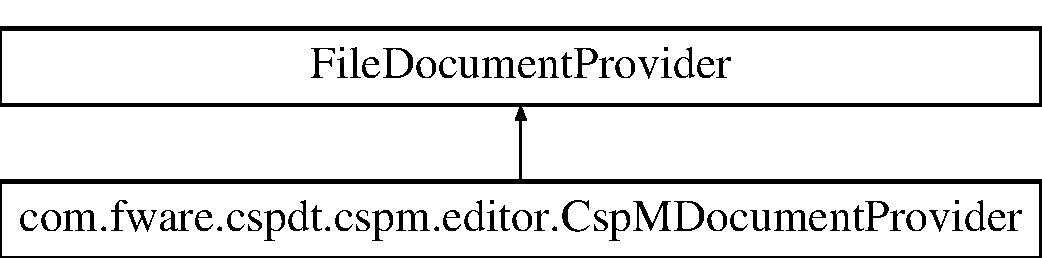
\includegraphics[height=2.000000cm]{classcom_1_1fware_1_1cspdt_1_1cspm_1_1editor_1_1_csp_m_document_provider}
\end{center}
\end{figure}
\subsection*{Protected Member Functions}
\begin{DoxyCompactItemize}
\item 
I\+Document \hyperlink{classcom_1_1fware_1_1cspdt_1_1cspm_1_1editor_1_1_csp_m_document_provider_aee079461064a45daaf96dcfd68df8ea1}{create\+Document} (Object element)  throws Core\+Exception 
\end{DoxyCompactItemize}


\subsection{Detailed Description}
Esta classe faz a representacao textual de um arquivo armazenado no diretorio do projeto. 

Atraves desta classe pode-\/se abrir o arquivo no editor realizar as edicoes no seu conteudo e monitorar todas as modificoes feitas desde seu carregamento.

\begin{DoxyAuthor}{Author}
A\+L\+V\+A\+RO, E\+V\+E\+R\+A\+L\+DA, F\+E\+L\+I\+PE, J\+O\+N\+A\+T\+H\+AN, J\+U\+V\+E\+N\+AL 
\end{DoxyAuthor}


\subsection{Member Function Documentation}
\mbox{\Hypertarget{classcom_1_1fware_1_1cspdt_1_1cspm_1_1editor_1_1_csp_m_document_provider_aee079461064a45daaf96dcfd68df8ea1}\label{classcom_1_1fware_1_1cspdt_1_1cspm_1_1editor_1_1_csp_m_document_provider_aee079461064a45daaf96dcfd68df8ea1}} 
\index{com\+::fware\+::cspdt\+::cspm\+::editor\+::\+Csp\+M\+Document\+Provider@{com\+::fware\+::cspdt\+::cspm\+::editor\+::\+Csp\+M\+Document\+Provider}!create\+Document@{create\+Document}}
\index{create\+Document@{create\+Document}!com\+::fware\+::cspdt\+::cspm\+::editor\+::\+Csp\+M\+Document\+Provider@{com\+::fware\+::cspdt\+::cspm\+::editor\+::\+Csp\+M\+Document\+Provider}}
\subsubsection{\texorpdfstring{create\+Document()}{createDocument()}}
{\footnotesize\ttfamily I\+Document com.\+fware.\+cspdt.\+cspm.\+editor.\+Csp\+M\+Document\+Provider.\+create\+Document (\begin{DoxyParamCaption}\item[{Object}]{element }\end{DoxyParamCaption}) throws Core\+Exception\hspace{0.3cm}{\ttfamily [inline]}, {\ttfamily [protected]}}

\begin{DoxySeeAlso}{See also}
org.\+eclipse.\+ui.\+editors.\+text.\+File\+Document\+Provider\+::create\+Document() 
\end{DoxySeeAlso}


The documentation for this class was generated from the following file\+:\begin{DoxyCompactItemize}
\item 
C\+:/\+Users/\+E\+V\+A/\+Downloads/eclipse/workspace/cspdt/com.\+fware.\+cspdt.\+cspm.\+editor/src/com/fware/cspdt/cspm/editor/Csp\+M\+Document\+Provider.\+java\end{DoxyCompactItemize}

\hypertarget{classcom_1_1fware_1_1cspdt_1_1cspm_1_1editor_1_1config_1_1_csp_m_double_click_strategy}{}\section{com.\+fware.\+cspdt.\+cspm.\+editor.\+config.\+Csp\+M\+Double\+Click\+Strategy Class Reference}
\label{classcom_1_1fware_1_1cspdt_1_1cspm_1_1editor_1_1config_1_1_csp_m_double_click_strategy}\index{com.\+fware.\+cspdt.\+cspm.\+editor.\+config.\+Csp\+M\+Double\+Click\+Strategy@{com.\+fware.\+cspdt.\+cspm.\+editor.\+config.\+Csp\+M\+Double\+Click\+Strategy}}


Esta classe cria uma estrategia de acao para o clique duplo no codigo C\+S\+PM.  


Inheritance diagram for com.\+fware.\+cspdt.\+cspm.\+editor.\+config.\+Csp\+M\+Double\+Click\+Strategy\+:\begin{figure}[H]
\begin{center}
\leavevmode
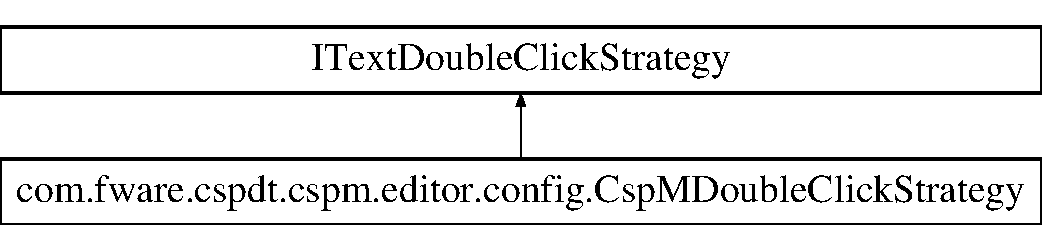
\includegraphics[height=2.000000cm]{classcom_1_1fware_1_1cspdt_1_1cspm_1_1editor_1_1config_1_1_csp_m_double_click_strategy}
\end{center}
\end{figure}
\subsection*{Public Member Functions}
\begin{DoxyCompactItemize}
\item 
void \hyperlink{classcom_1_1fware_1_1cspdt_1_1cspm_1_1editor_1_1config_1_1_csp_m_double_click_strategy_a0e4b88b8359d976abf366b46705eb55c}{double\+Clicked} (I\+Text\+Viewer part)
\begin{DoxyCompactList}\small\item\em Acao do clique duplo no editor de texto. \end{DoxyCompactList}\end{DoxyCompactItemize}
\subsection*{Protected Member Functions}
\begin{DoxyCompactItemize}
\item 
\mbox{\Hypertarget{classcom_1_1fware_1_1cspdt_1_1cspm_1_1editor_1_1config_1_1_csp_m_double_click_strategy_af4c4d72a869a3940954dc9e88582cd81}\label{classcom_1_1fware_1_1cspdt_1_1cspm_1_1editor_1_1config_1_1_csp_m_double_click_strategy_af4c4d72a869a3940954dc9e88582cd81}} 
boolean {\bfseries select\+Comment} (int caret\+Pos)
\item 
\mbox{\Hypertarget{classcom_1_1fware_1_1cspdt_1_1cspm_1_1editor_1_1config_1_1_csp_m_double_click_strategy_ac9cb7bcc033279d70e452189958cf83a}\label{classcom_1_1fware_1_1cspdt_1_1cspm_1_1editor_1_1config_1_1_csp_m_double_click_strategy_ac9cb7bcc033279d70e452189958cf83a}} 
boolean {\bfseries select\+Word} (int caret\+Pos)
\end{DoxyCompactItemize}
\subsection*{Protected Attributes}
\begin{DoxyCompactItemize}
\item 
\mbox{\Hypertarget{classcom_1_1fware_1_1cspdt_1_1cspm_1_1editor_1_1config_1_1_csp_m_double_click_strategy_ae198a896bfb74826e91d029255703f30}\label{classcom_1_1fware_1_1cspdt_1_1cspm_1_1editor_1_1config_1_1_csp_m_double_click_strategy_ae198a896bfb74826e91d029255703f30}} 
I\+Text\+Viewer {\bfseries f\+Text}
\end{DoxyCompactItemize}


\subsection{Detailed Description}
Esta classe cria uma estrategia de acao para o clique duplo no codigo C\+S\+PM. 

\begin{DoxyAuthor}{Author}
A\+L\+V\+A\+RO, E\+V\+E\+R\+A\+L\+DA, F\+E\+L\+I\+PE, J\+O\+N\+A\+T\+H\+AN, J\+U\+V\+E\+N\+AL 
\end{DoxyAuthor}


\subsection{Member Function Documentation}
\mbox{\Hypertarget{classcom_1_1fware_1_1cspdt_1_1cspm_1_1editor_1_1config_1_1_csp_m_double_click_strategy_a0e4b88b8359d976abf366b46705eb55c}\label{classcom_1_1fware_1_1cspdt_1_1cspm_1_1editor_1_1config_1_1_csp_m_double_click_strategy_a0e4b88b8359d976abf366b46705eb55c}} 
\index{com\+::fware\+::cspdt\+::cspm\+::editor\+::config\+::\+Csp\+M\+Double\+Click\+Strategy@{com\+::fware\+::cspdt\+::cspm\+::editor\+::config\+::\+Csp\+M\+Double\+Click\+Strategy}!double\+Clicked@{double\+Clicked}}
\index{double\+Clicked@{double\+Clicked}!com\+::fware\+::cspdt\+::cspm\+::editor\+::config\+::\+Csp\+M\+Double\+Click\+Strategy@{com\+::fware\+::cspdt\+::cspm\+::editor\+::config\+::\+Csp\+M\+Double\+Click\+Strategy}}
\subsubsection{\texorpdfstring{double\+Clicked()}{doubleClicked()}}
{\footnotesize\ttfamily void com.\+fware.\+cspdt.\+cspm.\+editor.\+config.\+Csp\+M\+Double\+Click\+Strategy.\+double\+Clicked (\begin{DoxyParamCaption}\item[{I\+Text\+Viewer}]{part }\end{DoxyParamCaption})\hspace{0.3cm}{\ttfamily [inline]}}



Acao do clique duplo no editor de texto. 

Esse metodo demarca o que sera selecionado no clique duplo. 

The documentation for this class was generated from the following file\+:\begin{DoxyCompactItemize}
\item 
C\+:/\+Users/\+E\+V\+A/\+Downloads/eclipse/workspace/cspdt/com.\+fware.\+cspdt.\+cspm.\+editor/src/com/fware/cspdt/cspm/editor/config/Csp\+M\+Double\+Click\+Strategy.\+java\end{DoxyCompactItemize}

\hypertarget{classcom_1_1fware_1_1cspdt_1_1cspm_1_1editor_1_1_csp_m_editor}{}\section{com.\+fware.\+cspdt.\+cspm.\+editor.\+Csp\+M\+Editor Class Reference}
\label{classcom_1_1fware_1_1cspdt_1_1cspm_1_1editor_1_1_csp_m_editor}\index{com.\+fware.\+cspdt.\+cspm.\+editor.\+Csp\+M\+Editor@{com.\+fware.\+cspdt.\+cspm.\+editor.\+Csp\+M\+Editor}}


Editor de texto para o C\+S\+PM.  


Inheritance diagram for com.\+fware.\+cspdt.\+cspm.\+editor.\+Csp\+M\+Editor\+:\begin{figure}[H]
\begin{center}
\leavevmode
\includegraphics[height=2.000000cm]{classcom_1_1fware_1_1cspdt_1_1cspm_1_1editor_1_1_csp_m_editor}
\end{center}
\end{figure}
\subsection*{Public Member Functions}
\begin{DoxyCompactItemize}
\item 
\mbox{\Hypertarget{classcom_1_1fware_1_1cspdt_1_1cspm_1_1editor_1_1_csp_m_editor_aa673dd146d99b9bf56daacc13c406c17}\label{classcom_1_1fware_1_1cspdt_1_1cspm_1_1editor_1_1_csp_m_editor_aa673dd146d99b9bf56daacc13c406c17}} 
\hyperlink{classcom_1_1fware_1_1cspdt_1_1cspm_1_1editor_1_1_csp_m_editor_aa673dd146d99b9bf56daacc13c406c17}{Csp\+M\+Editor} ()
\begin{DoxyCompactList}\small\item\em Constructor. \end{DoxyCompactList}\item 
\mbox{\Hypertarget{classcom_1_1fware_1_1cspdt_1_1cspm_1_1editor_1_1_csp_m_editor_a23448f05aa862609dfb4142e906b6fd7}\label{classcom_1_1fware_1_1cspdt_1_1cspm_1_1editor_1_1_csp_m_editor_a23448f05aa862609dfb4142e906b6fd7}} 
\hyperlink{classcom_1_1fware_1_1cspdt_1_1cspm_1_1editor_1_1config_1_1_csp_m_color_manager}{Csp\+M\+Color\+Manager} {\bfseries get\+Color\+Manager} ()
\item 
\mbox{\Hypertarget{classcom_1_1fware_1_1cspdt_1_1cspm_1_1editor_1_1_csp_m_editor_a6dc2f55df160a1d843a040e7eaf0c37a}\label{classcom_1_1fware_1_1cspdt_1_1cspm_1_1editor_1_1_csp_m_editor_a6dc2f55df160a1d843a040e7eaf0c37a}} 
I\+Token\+Scanner {\bfseries get\+Csp\+M\+Scanner} ()
\item 
\mbox{\Hypertarget{classcom_1_1fware_1_1cspdt_1_1cspm_1_1editor_1_1_csp_m_editor_a3b7d93cd97f3f60e52faf0b21fefa460}\label{classcom_1_1fware_1_1cspdt_1_1cspm_1_1editor_1_1_csp_m_editor_a3b7d93cd97f3f60e52faf0b21fefa460}} 
I\+Token\+Scanner {\bfseries get\+Csp\+Comment\+Scanner} ()
\item 
\mbox{\Hypertarget{classcom_1_1fware_1_1cspdt_1_1cspm_1_1editor_1_1_csp_m_editor_ababdba092d67fe17fac118fa3ddff9bc}\label{classcom_1_1fware_1_1cspdt_1_1cspm_1_1editor_1_1_csp_m_editor_ababdba092d67fe17fac118fa3ddff9bc}} 
I\+Token\+Scanner {\bfseries get\+Csp\+Multi\+Line\+Comment\+Scanner} ()
\item 
Object \hyperlink{classcom_1_1fware_1_1cspdt_1_1cspm_1_1editor_1_1_csp_m_editor_a2db9cb46fa80fad64bdb46c6c74672e6}{get\+Adapter} (Class required)
\item 
\mbox{\Hypertarget{classcom_1_1fware_1_1cspdt_1_1cspm_1_1editor_1_1_csp_m_editor_a92b685971bde7a66537b16daa6af4a52}\label{classcom_1_1fware_1_1cspdt_1_1cspm_1_1editor_1_1_csp_m_editor_a92b685971bde7a66537b16daa6af4a52}} 
I\+Document {\bfseries get\+Document} ()
\item 
void \hyperlink{classcom_1_1fware_1_1cspdt_1_1cspm_1_1editor_1_1_csp_m_editor_ac418cf2c7e96b563d27c3acf127ec1cb}{dispose} ()
\item 
\mbox{\Hypertarget{classcom_1_1fware_1_1cspdt_1_1cspm_1_1editor_1_1_csp_m_editor_a756a5c72d5fb29ce9755892392e7aa65}\label{classcom_1_1fware_1_1cspdt_1_1cspm_1_1editor_1_1_csp_m_editor_a756a5c72d5fb29ce9755892392e7aa65}} 
I\+Source\+Viewer {\bfseries get\+Viewer} ()
\item 
\mbox{\Hypertarget{classcom_1_1fware_1_1cspdt_1_1cspm_1_1editor_1_1_csp_m_editor_ac9ab0ff6658265253f92d3a20181d2d1}\label{classcom_1_1fware_1_1cspdt_1_1cspm_1_1editor_1_1_csp_m_editor_ac9ab0ff6658265253f92d3a20181d2d1}} 
Style\+Range {\bfseries get\+Under\+Line\+Range} ()
\item 
\mbox{\Hypertarget{classcom_1_1fware_1_1cspdt_1_1cspm_1_1editor_1_1_csp_m_editor_a144d495291f4717d7c5f36ceabefac93}\label{classcom_1_1fware_1_1cspdt_1_1cspm_1_1editor_1_1_csp_m_editor_a144d495291f4717d7c5f36ceabefac93}} 
void {\bfseries set\+Under\+Line\+Range} (Style\+Range under\+Line\+Range)
\item 
\mbox{\Hypertarget{classcom_1_1fware_1_1cspdt_1_1cspm_1_1editor_1_1_csp_m_editor_a895b1a97641241786ef7f7f74b678f07}\label{classcom_1_1fware_1_1cspdt_1_1cspm_1_1editor_1_1_csp_m_editor_a895b1a97641241786ef7f7f74b678f07}} 
Csp\+M\+Parser {\bfseries get\+Parser} ()
\item 
Csp\+M\+Model \hyperlink{classcom_1_1fware_1_1cspdt_1_1cspm_1_1editor_1_1_csp_m_editor_a8507980bcb241d6990f3c21c78380c32}{parse} ()
\begin{DoxyCompactList}\small\item\em Metodo responsavel para a geracao da arvore sintatica (A\+ST). \end{DoxyCompactList}\item 
\mbox{\Hypertarget{classcom_1_1fware_1_1cspdt_1_1cspm_1_1editor_1_1_csp_m_editor_ab760376d978f7985102f1ba62326b763}\label{classcom_1_1fware_1_1cspdt_1_1cspm_1_1editor_1_1_csp_m_editor_ab760376d978f7985102f1ba62326b763}} 
\hyperlink{classcom_1_1fware_1_1cspdt_1_1cspm_1_1editor_1_1marker_1_1_csp_m_marking_error_handler}{Csp\+M\+Marking\+Error\+Handler} {\bfseries get\+Marking\+Error\+Handler} ()
\item 
\mbox{\Hypertarget{classcom_1_1fware_1_1cspdt_1_1cspm_1_1editor_1_1_csp_m_editor_a59af88045ea8062603b190e05365a5c4}\label{classcom_1_1fware_1_1cspdt_1_1cspm_1_1editor_1_1_csp_m_editor_a59af88045ea8062603b190e05365a5c4}} 
void {\bfseries do\+Revert\+To\+Saved} ()
\item 
\mbox{\Hypertarget{classcom_1_1fware_1_1cspdt_1_1cspm_1_1editor_1_1_csp_m_editor_af040d0153687c664e603aa5212b1766a}\label{classcom_1_1fware_1_1cspdt_1_1cspm_1_1editor_1_1_csp_m_editor_af040d0153687c664e603aa5212b1766a}} 
void {\bfseries do\+Save} (I\+Progress\+Monitor monitor)
\item 
\mbox{\Hypertarget{classcom_1_1fware_1_1cspdt_1_1cspm_1_1editor_1_1_csp_m_editor_a9f3057611bc4be7cbab5379c007b601a}\label{classcom_1_1fware_1_1cspdt_1_1cspm_1_1editor_1_1_csp_m_editor_a9f3057611bc4be7cbab5379c007b601a}} 
void {\bfseries do\+Save\+As} ()
\item 
\mbox{\Hypertarget{classcom_1_1fware_1_1cspdt_1_1cspm_1_1editor_1_1_csp_m_editor_aa5065b94c9b663c467c61a6abc18cb5f}\label{classcom_1_1fware_1_1cspdt_1_1cspm_1_1editor_1_1_csp_m_editor_aa5065b94c9b663c467c61a6abc18cb5f}} 
void {\bfseries do\+Set\+Input} (I\+Editor\+Input input)  throws Core\+Exception 
\item 
\mbox{\Hypertarget{classcom_1_1fware_1_1cspdt_1_1cspm_1_1editor_1_1_csp_m_editor_a5acfd1c735b4e25cd3a0c51f6ff01034}\label{classcom_1_1fware_1_1cspdt_1_1cspm_1_1editor_1_1_csp_m_editor_a5acfd1c735b4e25cd3a0c51f6ff01034}} 
I\+Editor\+Input {\bfseries get\+Input} ()
\item 
\mbox{\Hypertarget{classcom_1_1fware_1_1cspdt_1_1cspm_1_1editor_1_1_csp_m_editor_a6ddd69ff4ac6af5857404bdddf6ca66f}\label{classcom_1_1fware_1_1cspdt_1_1cspm_1_1editor_1_1_csp_m_editor_a6ddd69ff4ac6af5857404bdddf6ca66f}} 
I\+File {\bfseries get\+Input\+File} ()
\end{DoxyCompactItemize}
\subsection*{Static Public Member Functions}
\begin{DoxyCompactItemize}
\item 
\mbox{\Hypertarget{classcom_1_1fware_1_1cspdt_1_1cspm_1_1editor_1_1_csp_m_editor_a78fb9858c965be2dc3dbdda779c89fb6}\label{classcom_1_1fware_1_1cspdt_1_1cspm_1_1editor_1_1_csp_m_editor_a78fb9858c965be2dc3dbdda779c89fb6}} 
static I\+Partition\+Token\+Scanner {\bfseries get\+Csp\+Partition\+Scanner} ()
\end{DoxyCompactItemize}
\subsection*{Protected Member Functions}
\begin{DoxyCompactItemize}
\item 
void \hyperlink{classcom_1_1fware_1_1cspdt_1_1cspm_1_1editor_1_1_csp_m_editor_a5a7ce7c7cb07830ab01c15728a543347}{initialize\+Editor} ()
\item 
\mbox{\Hypertarget{classcom_1_1fware_1_1cspdt_1_1cspm_1_1editor_1_1_csp_m_editor_ac89083d7cfdb1f57d2541845e61a7941}\label{classcom_1_1fware_1_1cspdt_1_1cspm_1_1editor_1_1_csp_m_editor_ac89083d7cfdb1f57d2541845e61a7941}} 
I\+Document {\bfseries get\+Input\+Document} ()
\end{DoxyCompactItemize}


\subsection{Detailed Description}
Editor de texto para o C\+S\+PM. 

Descreve o ambiente onde os codigos C\+S\+MP serao escritos

\begin{DoxyAuthor}{Author}
Joabe Jesus (\href{mailto:jbjj@cin.ufpe.br}{\tt jbjj@cin.\+ufpe.\+br}) 
\end{DoxyAuthor}


\subsection{Member Function Documentation}
\mbox{\Hypertarget{classcom_1_1fware_1_1cspdt_1_1cspm_1_1editor_1_1_csp_m_editor_ac418cf2c7e96b563d27c3acf127ec1cb}\label{classcom_1_1fware_1_1cspdt_1_1cspm_1_1editor_1_1_csp_m_editor_ac418cf2c7e96b563d27c3acf127ec1cb}} 
\index{com\+::fware\+::cspdt\+::cspm\+::editor\+::\+Csp\+M\+Editor@{com\+::fware\+::cspdt\+::cspm\+::editor\+::\+Csp\+M\+Editor}!dispose@{dispose}}
\index{dispose@{dispose}!com\+::fware\+::cspdt\+::cspm\+::editor\+::\+Csp\+M\+Editor@{com\+::fware\+::cspdt\+::cspm\+::editor\+::\+Csp\+M\+Editor}}
\subsubsection{\texorpdfstring{dispose()}{dispose()}}
{\footnotesize\ttfamily void com.\+fware.\+cspdt.\+cspm.\+editor.\+Csp\+M\+Editor.\+dispose (\begin{DoxyParamCaption}{ }\end{DoxyParamCaption})\hspace{0.3cm}{\ttfamily [inline]}}

\begin{DoxySeeAlso}{See also}
org.\+eclipse.\+ui.\+editors.\+text.\+Text\+Editor\+::dispose() 
\end{DoxySeeAlso}
\mbox{\Hypertarget{classcom_1_1fware_1_1cspdt_1_1cspm_1_1editor_1_1_csp_m_editor_a2db9cb46fa80fad64bdb46c6c74672e6}\label{classcom_1_1fware_1_1cspdt_1_1cspm_1_1editor_1_1_csp_m_editor_a2db9cb46fa80fad64bdb46c6c74672e6}} 
\index{com\+::fware\+::cspdt\+::cspm\+::editor\+::\+Csp\+M\+Editor@{com\+::fware\+::cspdt\+::cspm\+::editor\+::\+Csp\+M\+Editor}!get\+Adapter@{get\+Adapter}}
\index{get\+Adapter@{get\+Adapter}!com\+::fware\+::cspdt\+::cspm\+::editor\+::\+Csp\+M\+Editor@{com\+::fware\+::cspdt\+::cspm\+::editor\+::\+Csp\+M\+Editor}}
\subsubsection{\texorpdfstring{get\+Adapter()}{getAdapter()}}
{\footnotesize\ttfamily Object com.\+fware.\+cspdt.\+cspm.\+editor.\+Csp\+M\+Editor.\+get\+Adapter (\begin{DoxyParamCaption}\item[{Class}]{required }\end{DoxyParamCaption})\hspace{0.3cm}{\ttfamily [inline]}}

\begin{DoxySeeAlso}{See also}
org.\+eclipse.\+ui.\+editors.\+text.\+Text\+Editor\+::get\+Adapter() 
\end{DoxySeeAlso}
\mbox{\Hypertarget{classcom_1_1fware_1_1cspdt_1_1cspm_1_1editor_1_1_csp_m_editor_a5a7ce7c7cb07830ab01c15728a543347}\label{classcom_1_1fware_1_1cspdt_1_1cspm_1_1editor_1_1_csp_m_editor_a5a7ce7c7cb07830ab01c15728a543347}} 
\index{com\+::fware\+::cspdt\+::cspm\+::editor\+::\+Csp\+M\+Editor@{com\+::fware\+::cspdt\+::cspm\+::editor\+::\+Csp\+M\+Editor}!initialize\+Editor@{initialize\+Editor}}
\index{initialize\+Editor@{initialize\+Editor}!com\+::fware\+::cspdt\+::cspm\+::editor\+::\+Csp\+M\+Editor@{com\+::fware\+::cspdt\+::cspm\+::editor\+::\+Csp\+M\+Editor}}
\subsubsection{\texorpdfstring{initialize\+Editor()}{initializeEditor()}}
{\footnotesize\ttfamily void com.\+fware.\+cspdt.\+cspm.\+editor.\+Csp\+M\+Editor.\+initialize\+Editor (\begin{DoxyParamCaption}{ }\end{DoxyParamCaption})\hspace{0.3cm}{\ttfamily [inline]}, {\ttfamily [protected]}}

\begin{DoxySeeAlso}{See also}
org.\+eclipse.\+ui.\+editors.\+text.\+Text\+Editor\+::initialize\+Editor() 
\end{DoxySeeAlso}
\mbox{\Hypertarget{classcom_1_1fware_1_1cspdt_1_1cspm_1_1editor_1_1_csp_m_editor_a8507980bcb241d6990f3c21c78380c32}\label{classcom_1_1fware_1_1cspdt_1_1cspm_1_1editor_1_1_csp_m_editor_a8507980bcb241d6990f3c21c78380c32}} 
\index{com\+::fware\+::cspdt\+::cspm\+::editor\+::\+Csp\+M\+Editor@{com\+::fware\+::cspdt\+::cspm\+::editor\+::\+Csp\+M\+Editor}!parse@{parse}}
\index{parse@{parse}!com\+::fware\+::cspdt\+::cspm\+::editor\+::\+Csp\+M\+Editor@{com\+::fware\+::cspdt\+::cspm\+::editor\+::\+Csp\+M\+Editor}}
\subsubsection{\texorpdfstring{parse()}{parse()}}
{\footnotesize\ttfamily Csp\+M\+Model com.\+fware.\+cspdt.\+cspm.\+editor.\+Csp\+M\+Editor.\+parse (\begin{DoxyParamCaption}{ }\end{DoxyParamCaption})\hspace{0.3cm}{\ttfamily [inline]}}



Metodo responsavel para a geracao da arvore sintatica (A\+ST). 

Este metodo executa o get\+Info() do Csp\+M\+Parser que gera a A\+ST e tambem faz a geracao de marcadores de erro no codigo.

\begin{DoxyReturn}{Returns}
O modelo criado pela analise do codigo 
\end{DoxyReturn}


The documentation for this class was generated from the following file\+:\begin{DoxyCompactItemize}
\item 
C\+:/\+Users/\+E\+V\+A/\+Downloads/eclipse/workspace/cspdt/com.\+fware.\+cspdt.\+cspm.\+editor/src/com/fware/cspdt/cspm/editor/Csp\+M\+Editor.\+java\end{DoxyCompactItemize}

\hypertarget{classcom_1_1fware_1_1cspdt_1_1cspm_1_1editor_1_1_csp_m_editor_plugin}{}\section{com.\+fware.\+cspdt.\+cspm.\+editor.\+Csp\+M\+Editor\+Plugin Class Reference}
\label{classcom_1_1fware_1_1cspdt_1_1cspm_1_1editor_1_1_csp_m_editor_plugin}\index{com.\+fware.\+cspdt.\+cspm.\+editor.\+Csp\+M\+Editor\+Plugin@{com.\+fware.\+cspdt.\+cspm.\+editor.\+Csp\+M\+Editor\+Plugin}}


The activator class controls the plug-\/in life cycle.  


Inheritance diagram for com.\+fware.\+cspdt.\+cspm.\+editor.\+Csp\+M\+Editor\+Plugin\+:\begin{figure}[H]
\begin{center}
\leavevmode
\includegraphics[height=2.000000cm]{classcom_1_1fware_1_1cspdt_1_1cspm_1_1editor_1_1_csp_m_editor_plugin}
\end{center}
\end{figure}
\subsection*{Public Member Functions}
\begin{DoxyCompactItemize}
\item 
\mbox{\Hypertarget{classcom_1_1fware_1_1cspdt_1_1cspm_1_1editor_1_1_csp_m_editor_plugin_a132fdd00e0ab589fd1e0cf2469cb3b88}\label{classcom_1_1fware_1_1cspdt_1_1cspm_1_1editor_1_1_csp_m_editor_plugin_a132fdd00e0ab589fd1e0cf2469cb3b88}} 
\hyperlink{classcom_1_1fware_1_1cspdt_1_1cspm_1_1editor_1_1_csp_m_editor_plugin_a132fdd00e0ab589fd1e0cf2469cb3b88}{Csp\+M\+Editor\+Plugin} ()
\begin{DoxyCompactList}\small\item\em Constructs a new C\+SP S\+U\+I\+TE plugin object. \end{DoxyCompactList}\item 
\mbox{\Hypertarget{classcom_1_1fware_1_1cspdt_1_1cspm_1_1editor_1_1_csp_m_editor_plugin_a8bcd3b653eb143f50f9584e3ba6d426e}\label{classcom_1_1fware_1_1cspdt_1_1cspm_1_1editor_1_1_csp_m_editor_plugin_a8bcd3b653eb143f50f9584e3ba6d426e}} 
void {\bfseries start} (Bundle\+Context context)  throws Exception 
\item 
\mbox{\Hypertarget{classcom_1_1fware_1_1cspdt_1_1cspm_1_1editor_1_1_csp_m_editor_plugin_aec8977bf750ac404c55cf9e3998c0343}\label{classcom_1_1fware_1_1cspdt_1_1cspm_1_1editor_1_1_csp_m_editor_plugin_aec8977bf750ac404c55cf9e3998c0343}} 
void {\bfseries stop} (Bundle\+Context context)  throws Exception 
\end{DoxyCompactItemize}
\subsection*{Static Public Member Functions}
\begin{DoxyCompactItemize}
\item 
static \hyperlink{classcom_1_1fware_1_1cspdt_1_1cspm_1_1editor_1_1_csp_m_editor_plugin}{Csp\+M\+Editor\+Plugin} \hyperlink{classcom_1_1fware_1_1cspdt_1_1cspm_1_1editor_1_1_csp_m_editor_plugin_a5809344c36c4947f0f4cbe01d7daf633}{get\+Default} ()
\begin{DoxyCompactList}\small\item\em Returns the shared instance. \end{DoxyCompactList}\item 
static String \hyperlink{classcom_1_1fware_1_1cspdt_1_1cspm_1_1editor_1_1_csp_m_editor_plugin_a3108b6f331629b6acb68b8f9e7987fd0}{get\+Plugin\+Id} ()
\begin{DoxyCompactList}\small\item\em Returns the name of the plugin. \end{DoxyCompactList}\item 
static String \hyperlink{classcom_1_1fware_1_1cspdt_1_1cspm_1_1editor_1_1_csp_m_editor_plugin_a7d802c2a09d9e2a3fd8c69f76485e19f}{get\+Preference} (String key)
\begin{DoxyCompactList}\small\item\em Return a value from the plugin\textquotesingle{}s preferences. \end{DoxyCompactList}\item 
static Image \hyperlink{classcom_1_1fware_1_1cspdt_1_1cspm_1_1editor_1_1_csp_m_editor_plugin_a617d7093508af7b8925513888ba9abaa}{get\+Image} (String name)
\begin{DoxyCompactList}\small\item\em Return an image from the plugin\textquotesingle{}s icons-\/directory. \end{DoxyCompactList}\item 
static Image\+Descriptor \hyperlink{classcom_1_1fware_1_1cspdt_1_1cspm_1_1editor_1_1_csp_m_editor_plugin_ac421550bc116a9d99997fa22d1fd45ab}{get\+Image\+Descriptor} (String path)
\begin{DoxyCompactList}\small\item\em Returns an image descriptor for the image file at the given plug-\/in relative path (from eclipse help). \end{DoxyCompactList}\item 
static I\+Workbench\+Page \hyperlink{classcom_1_1fware_1_1cspdt_1_1cspm_1_1editor_1_1_csp_m_editor_plugin_a42cad1fb2c902c98a3e479bd45c6e0ab}{get\+Current\+Workbench\+Page} ()
\begin{DoxyCompactList}\small\item\em Returns the current workbench page. \end{DoxyCompactList}\item 
static I\+Status \hyperlink{classcom_1_1fware_1_1cspdt_1_1cspm_1_1editor_1_1_csp_m_editor_plugin_a5b396412e4eaff95c0edf8b65ea055fd}{stat} (String msg)
\begin{DoxyCompactList}\small\item\em This is equivalent to calling {\ttfamily stat(msg, null)}. \end{DoxyCompactList}\item 
static I\+Status \hyperlink{classcom_1_1fware_1_1cspdt_1_1cspm_1_1editor_1_1_csp_m_editor_plugin_a8f6c15a840760c132d98bbae18564db3}{stat} (String msg, Throwable t)
\begin{DoxyCompactList}\small\item\em Create an error-\/level status object out of textual message. \end{DoxyCompactList}\item 
static void \hyperlink{classcom_1_1fware_1_1cspdt_1_1cspm_1_1editor_1_1_csp_m_editor_plugin_a54650677eefb50d1f6f2a6ba7a76f81c}{log} (String msg, Throwable t)
\begin{DoxyCompactList}\small\item\em Display a message in the Eclipse\textquotesingle{}s Error Log. \end{DoxyCompactList}\item 
static void \hyperlink{classcom_1_1fware_1_1cspdt_1_1cspm_1_1editor_1_1_csp_m_editor_plugin_a2c4fa5b39642bfadc3af60a6ea74065c}{log} (String msg, Throwable t, int level)
\begin{DoxyCompactList}\small\item\em Display a message in the Eclipse\textquotesingle{}s Error Log. \end{DoxyCompactList}\end{DoxyCompactItemize}
\subsection*{Static Public Attributes}
\begin{DoxyCompactItemize}
\item 
static final String \hyperlink{classcom_1_1fware_1_1cspdt_1_1cspm_1_1editor_1_1_csp_m_editor_plugin_a52beb6e08f5faf5ef31066ebb304d825}{P\+L\+U\+G\+I\+N\+\_\+\+ID} = \char`\"{}Csp\+Suite\char`\"{}
\begin{DoxyCompactList}\small\item\em The plug-\/in ID. \end{DoxyCompactList}\end{DoxyCompactItemize}
\subsection*{Protected Member Functions}
\begin{DoxyCompactItemize}
\item 
Image \hyperlink{classcom_1_1fware_1_1cspdt_1_1cspm_1_1editor_1_1_csp_m_editor_plugin_a2386db9ed985b9049c0ba90a3fbf8695}{get\+Cached\+Image} (String key)
\begin{DoxyCompactList}\small\item\em Cache the image if it is found. \end{DoxyCompactList}\end{DoxyCompactItemize}
\subsection*{Static Protected Attributes}
\begin{DoxyCompactItemize}
\item 
static I\+Workbench\+Window \hyperlink{classcom_1_1fware_1_1cspdt_1_1cspm_1_1editor_1_1_csp_m_editor_plugin_a00372fb921d6f5cc3ee5b79bb1fa065a}{current\+Window}
\begin{DoxyCompactList}\small\item\em Used by the current project solving mechanism. \end{DoxyCompactList}\end{DoxyCompactItemize}


\subsection{Detailed Description}
The activator class controls the plug-\/in life cycle. 

\subsection{Member Function Documentation}
\mbox{\Hypertarget{classcom_1_1fware_1_1cspdt_1_1cspm_1_1editor_1_1_csp_m_editor_plugin_a2386db9ed985b9049c0ba90a3fbf8695}\label{classcom_1_1fware_1_1cspdt_1_1cspm_1_1editor_1_1_csp_m_editor_plugin_a2386db9ed985b9049c0ba90a3fbf8695}} 
\index{com\+::fware\+::cspdt\+::cspm\+::editor\+::\+Csp\+M\+Editor\+Plugin@{com\+::fware\+::cspdt\+::cspm\+::editor\+::\+Csp\+M\+Editor\+Plugin}!get\+Cached\+Image@{get\+Cached\+Image}}
\index{get\+Cached\+Image@{get\+Cached\+Image}!com\+::fware\+::cspdt\+::cspm\+::editor\+::\+Csp\+M\+Editor\+Plugin@{com\+::fware\+::cspdt\+::cspm\+::editor\+::\+Csp\+M\+Editor\+Plugin}}
\subsubsection{\texorpdfstring{get\+Cached\+Image()}{getCachedImage()}}
{\footnotesize\ttfamily Image com.\+fware.\+cspdt.\+cspm.\+editor.\+Csp\+M\+Editor\+Plugin.\+get\+Cached\+Image (\begin{DoxyParamCaption}\item[{String}]{key }\end{DoxyParamCaption})\hspace{0.3cm}{\ttfamily [inline]}, {\ttfamily [protected]}}



Cache the image if it is found. 


\begin{DoxyParams}{Parameters}
{\em key} & Name of the image \\
\hline
\end{DoxyParams}
\begin{DoxyReturn}{Returns}
Image from the cache or from disk, null if image is not found in either. 
\end{DoxyReturn}
\mbox{\Hypertarget{classcom_1_1fware_1_1cspdt_1_1cspm_1_1editor_1_1_csp_m_editor_plugin_a42cad1fb2c902c98a3e479bd45c6e0ab}\label{classcom_1_1fware_1_1cspdt_1_1cspm_1_1editor_1_1_csp_m_editor_plugin_a42cad1fb2c902c98a3e479bd45c6e0ab}} 
\index{com\+::fware\+::cspdt\+::cspm\+::editor\+::\+Csp\+M\+Editor\+Plugin@{com\+::fware\+::cspdt\+::cspm\+::editor\+::\+Csp\+M\+Editor\+Plugin}!get\+Current\+Workbench\+Page@{get\+Current\+Workbench\+Page}}
\index{get\+Current\+Workbench\+Page@{get\+Current\+Workbench\+Page}!com\+::fware\+::cspdt\+::cspm\+::editor\+::\+Csp\+M\+Editor\+Plugin@{com\+::fware\+::cspdt\+::cspm\+::editor\+::\+Csp\+M\+Editor\+Plugin}}
\subsubsection{\texorpdfstring{get\+Current\+Workbench\+Page()}{getCurrentWorkbenchPage()}}
{\footnotesize\ttfamily static I\+Workbench\+Page com.\+fware.\+cspdt.\+cspm.\+editor.\+Csp\+M\+Editor\+Plugin.\+get\+Current\+Workbench\+Page (\begin{DoxyParamCaption}{ }\end{DoxyParamCaption})\hspace{0.3cm}{\ttfamily [inline]}, {\ttfamily [static]}}



Returns the current workbench page. 

Used by get\+Current\+Project() and by goto\+Marker().

\begin{DoxyReturn}{Returns}
The currently open Workbench\+Page or {\ttfamily null} if none 
\end{DoxyReturn}
\mbox{\Hypertarget{classcom_1_1fware_1_1cspdt_1_1cspm_1_1editor_1_1_csp_m_editor_plugin_a5809344c36c4947f0f4cbe01d7daf633}\label{classcom_1_1fware_1_1cspdt_1_1cspm_1_1editor_1_1_csp_m_editor_plugin_a5809344c36c4947f0f4cbe01d7daf633}} 
\index{com\+::fware\+::cspdt\+::cspm\+::editor\+::\+Csp\+M\+Editor\+Plugin@{com\+::fware\+::cspdt\+::cspm\+::editor\+::\+Csp\+M\+Editor\+Plugin}!get\+Default@{get\+Default}}
\index{get\+Default@{get\+Default}!com\+::fware\+::cspdt\+::cspm\+::editor\+::\+Csp\+M\+Editor\+Plugin@{com\+::fware\+::cspdt\+::cspm\+::editor\+::\+Csp\+M\+Editor\+Plugin}}
\subsubsection{\texorpdfstring{get\+Default()}{getDefault()}}
{\footnotesize\ttfamily static \hyperlink{classcom_1_1fware_1_1cspdt_1_1cspm_1_1editor_1_1_csp_m_editor_plugin}{Csp\+M\+Editor\+Plugin} com.\+fware.\+cspdt.\+cspm.\+editor.\+Csp\+M\+Editor\+Plugin.\+get\+Default (\begin{DoxyParamCaption}{ }\end{DoxyParamCaption})\hspace{0.3cm}{\ttfamily [inline]}, {\ttfamily [static]}}



Returns the shared instance. 

\begin{DoxyReturn}{Returns}
the shared instance 
\end{DoxyReturn}
\mbox{\Hypertarget{classcom_1_1fware_1_1cspdt_1_1cspm_1_1editor_1_1_csp_m_editor_plugin_a617d7093508af7b8925513888ba9abaa}\label{classcom_1_1fware_1_1cspdt_1_1cspm_1_1editor_1_1_csp_m_editor_plugin_a617d7093508af7b8925513888ba9abaa}} 
\index{com\+::fware\+::cspdt\+::cspm\+::editor\+::\+Csp\+M\+Editor\+Plugin@{com\+::fware\+::cspdt\+::cspm\+::editor\+::\+Csp\+M\+Editor\+Plugin}!get\+Image@{get\+Image}}
\index{get\+Image@{get\+Image}!com\+::fware\+::cspdt\+::cspm\+::editor\+::\+Csp\+M\+Editor\+Plugin@{com\+::fware\+::cspdt\+::cspm\+::editor\+::\+Csp\+M\+Editor\+Plugin}}
\subsubsection{\texorpdfstring{get\+Image()}{getImage()}}
{\footnotesize\ttfamily static Image com.\+fware.\+cspdt.\+cspm.\+editor.\+Csp\+M\+Editor\+Plugin.\+get\+Image (\begin{DoxyParamCaption}\item[{String}]{name }\end{DoxyParamCaption})\hspace{0.3cm}{\ttfamily [inline]}, {\ttfamily [static]}}



Return an image from the plugin\textquotesingle{}s icons-\/directory. 


\begin{DoxyParams}{Parameters}
{\em name} & Name of the icon \\
\hline
\end{DoxyParams}
\begin{DoxyReturn}{Returns}
The icon as an image object 
\end{DoxyReturn}
\mbox{\Hypertarget{classcom_1_1fware_1_1cspdt_1_1cspm_1_1editor_1_1_csp_m_editor_plugin_ac421550bc116a9d99997fa22d1fd45ab}\label{classcom_1_1fware_1_1cspdt_1_1cspm_1_1editor_1_1_csp_m_editor_plugin_ac421550bc116a9d99997fa22d1fd45ab}} 
\index{com\+::fware\+::cspdt\+::cspm\+::editor\+::\+Csp\+M\+Editor\+Plugin@{com\+::fware\+::cspdt\+::cspm\+::editor\+::\+Csp\+M\+Editor\+Plugin}!get\+Image\+Descriptor@{get\+Image\+Descriptor}}
\index{get\+Image\+Descriptor@{get\+Image\+Descriptor}!com\+::fware\+::cspdt\+::cspm\+::editor\+::\+Csp\+M\+Editor\+Plugin@{com\+::fware\+::cspdt\+::cspm\+::editor\+::\+Csp\+M\+Editor\+Plugin}}
\subsubsection{\texorpdfstring{get\+Image\+Descriptor()}{getImageDescriptor()}}
{\footnotesize\ttfamily static Image\+Descriptor com.\+fware.\+cspdt.\+cspm.\+editor.\+Csp\+M\+Editor\+Plugin.\+get\+Image\+Descriptor (\begin{DoxyParamCaption}\item[{String}]{path }\end{DoxyParamCaption})\hspace{0.3cm}{\ttfamily [inline]}, {\ttfamily [static]}}



Returns an image descriptor for the image file at the given plug-\/in relative path (from eclipse help). 


\begin{DoxyParams}{Parameters}
{\em path} & Relative path of the image. \\
\hline
\end{DoxyParams}
\begin{DoxyReturn}{Returns}
The corresponding image descriptor or {\ttfamily Missing\+Image\+Descriptor} if none is found. 
\end{DoxyReturn}
\mbox{\Hypertarget{classcom_1_1fware_1_1cspdt_1_1cspm_1_1editor_1_1_csp_m_editor_plugin_a3108b6f331629b6acb68b8f9e7987fd0}\label{classcom_1_1fware_1_1cspdt_1_1cspm_1_1editor_1_1_csp_m_editor_plugin_a3108b6f331629b6acb68b8f9e7987fd0}} 
\index{com\+::fware\+::cspdt\+::cspm\+::editor\+::\+Csp\+M\+Editor\+Plugin@{com\+::fware\+::cspdt\+::cspm\+::editor\+::\+Csp\+M\+Editor\+Plugin}!get\+Plugin\+Id@{get\+Plugin\+Id}}
\index{get\+Plugin\+Id@{get\+Plugin\+Id}!com\+::fware\+::cspdt\+::cspm\+::editor\+::\+Csp\+M\+Editor\+Plugin@{com\+::fware\+::cspdt\+::cspm\+::editor\+::\+Csp\+M\+Editor\+Plugin}}
\subsubsection{\texorpdfstring{get\+Plugin\+Id()}{getPluginId()}}
{\footnotesize\ttfamily static String com.\+fware.\+cspdt.\+cspm.\+editor.\+Csp\+M\+Editor\+Plugin.\+get\+Plugin\+Id (\begin{DoxyParamCaption}{ }\end{DoxyParamCaption})\hspace{0.3cm}{\ttfamily [inline]}, {\ttfamily [static]}}



Returns the name of the plugin. 

Used by project creation wizard.

\begin{DoxyReturn}{Returns}
Unique id of this plugin 
\end{DoxyReturn}
\mbox{\Hypertarget{classcom_1_1fware_1_1cspdt_1_1cspm_1_1editor_1_1_csp_m_editor_plugin_a7d802c2a09d9e2a3fd8c69f76485e19f}\label{classcom_1_1fware_1_1cspdt_1_1cspm_1_1editor_1_1_csp_m_editor_plugin_a7d802c2a09d9e2a3fd8c69f76485e19f}} 
\index{com\+::fware\+::cspdt\+::cspm\+::editor\+::\+Csp\+M\+Editor\+Plugin@{com\+::fware\+::cspdt\+::cspm\+::editor\+::\+Csp\+M\+Editor\+Plugin}!get\+Preference@{get\+Preference}}
\index{get\+Preference@{get\+Preference}!com\+::fware\+::cspdt\+::cspm\+::editor\+::\+Csp\+M\+Editor\+Plugin@{com\+::fware\+::cspdt\+::cspm\+::editor\+::\+Csp\+M\+Editor\+Plugin}}
\subsubsection{\texorpdfstring{get\+Preference()}{getPreference()}}
{\footnotesize\ttfamily static String com.\+fware.\+cspdt.\+cspm.\+editor.\+Csp\+M\+Editor\+Plugin.\+get\+Preference (\begin{DoxyParamCaption}\item[{String}]{key }\end{DoxyParamCaption})\hspace{0.3cm}{\ttfamily [inline]}, {\ttfamily [static]}}



Return a value from the plugin\textquotesingle{}s preferences. 


\begin{DoxyParams}{Parameters}
{\em key} & Preference name \\
\hline
\end{DoxyParams}
\begin{DoxyReturn}{Returns}
Value of the named preference 
\end{DoxyReturn}
\mbox{\Hypertarget{classcom_1_1fware_1_1cspdt_1_1cspm_1_1editor_1_1_csp_m_editor_plugin_a54650677eefb50d1f6f2a6ba7a76f81c}\label{classcom_1_1fware_1_1cspdt_1_1cspm_1_1editor_1_1_csp_m_editor_plugin_a54650677eefb50d1f6f2a6ba7a76f81c}} 
\index{com\+::fware\+::cspdt\+::cspm\+::editor\+::\+Csp\+M\+Editor\+Plugin@{com\+::fware\+::cspdt\+::cspm\+::editor\+::\+Csp\+M\+Editor\+Plugin}!log@{log}}
\index{log@{log}!com\+::fware\+::cspdt\+::cspm\+::editor\+::\+Csp\+M\+Editor\+Plugin@{com\+::fware\+::cspdt\+::cspm\+::editor\+::\+Csp\+M\+Editor\+Plugin}}
\subsubsection{\texorpdfstring{log()}{log()}\hspace{0.1cm}{\footnotesize\ttfamily [1/2]}}
{\footnotesize\ttfamily static void com.\+fware.\+cspdt.\+cspm.\+editor.\+Csp\+M\+Editor\+Plugin.\+log (\begin{DoxyParamCaption}\item[{String}]{msg,  }\item[{Throwable}]{t }\end{DoxyParamCaption})\hspace{0.3cm}{\ttfamily [inline]}, {\ttfamily [static]}}



Display a message in the Eclipse\textquotesingle{}s Error Log. 

This is equivalent to calling {\ttfamily log(msg, t, I\+Status.\+E\+R\+R\+OR)}.


\begin{DoxyParams}{Parameters}
{\em msg} & Error message to display in error log \\
\hline
{\em t} & Exception \\
\hline
\end{DoxyParams}
\mbox{\Hypertarget{classcom_1_1fware_1_1cspdt_1_1cspm_1_1editor_1_1_csp_m_editor_plugin_a2c4fa5b39642bfadc3af60a6ea74065c}\label{classcom_1_1fware_1_1cspdt_1_1cspm_1_1editor_1_1_csp_m_editor_plugin_a2c4fa5b39642bfadc3af60a6ea74065c}} 
\index{com\+::fware\+::cspdt\+::cspm\+::editor\+::\+Csp\+M\+Editor\+Plugin@{com\+::fware\+::cspdt\+::cspm\+::editor\+::\+Csp\+M\+Editor\+Plugin}!log@{log}}
\index{log@{log}!com\+::fware\+::cspdt\+::cspm\+::editor\+::\+Csp\+M\+Editor\+Plugin@{com\+::fware\+::cspdt\+::cspm\+::editor\+::\+Csp\+M\+Editor\+Plugin}}
\subsubsection{\texorpdfstring{log()}{log()}\hspace{0.1cm}{\footnotesize\ttfamily [2/2]}}
{\footnotesize\ttfamily static void com.\+fware.\+cspdt.\+cspm.\+editor.\+Csp\+M\+Editor\+Plugin.\+log (\begin{DoxyParamCaption}\item[{String}]{msg,  }\item[{Throwable}]{t,  }\item[{int}]{level }\end{DoxyParamCaption})\hspace{0.3cm}{\ttfamily [inline]}, {\ttfamily [static]}}



Display a message in the Eclipse\textquotesingle{}s Error Log. 

Used by e.\+g. the project creation wizard.


\begin{DoxyParams}{Parameters}
{\em msg} & Error message \\
\hline
{\em t} & Exception \\
\hline
{\em level} & One of the error levels defined in the {\ttfamily I\+Status} -\/interface \\
\hline
\end{DoxyParams}
\mbox{\Hypertarget{classcom_1_1fware_1_1cspdt_1_1cspm_1_1editor_1_1_csp_m_editor_plugin_a5b396412e4eaff95c0edf8b65ea055fd}\label{classcom_1_1fware_1_1cspdt_1_1cspm_1_1editor_1_1_csp_m_editor_plugin_a5b396412e4eaff95c0edf8b65ea055fd}} 
\index{com\+::fware\+::cspdt\+::cspm\+::editor\+::\+Csp\+M\+Editor\+Plugin@{com\+::fware\+::cspdt\+::cspm\+::editor\+::\+Csp\+M\+Editor\+Plugin}!stat@{stat}}
\index{stat@{stat}!com\+::fware\+::cspdt\+::cspm\+::editor\+::\+Csp\+M\+Editor\+Plugin@{com\+::fware\+::cspdt\+::cspm\+::editor\+::\+Csp\+M\+Editor\+Plugin}}
\subsubsection{\texorpdfstring{stat()}{stat()}\hspace{0.1cm}{\footnotesize\ttfamily [1/2]}}
{\footnotesize\ttfamily static I\+Status com.\+fware.\+cspdt.\+cspm.\+editor.\+Csp\+M\+Editor\+Plugin.\+stat (\begin{DoxyParamCaption}\item[{String}]{msg }\end{DoxyParamCaption})\hspace{0.3cm}{\ttfamily [inline]}, {\ttfamily [static]}}



This is equivalent to calling {\ttfamily stat(msg, null)}. 


\begin{DoxyParams}{Parameters}
{\em msg} & Error message to display in error log \\
\hline
\end{DoxyParams}
\begin{DoxyReturn}{Returns}
New Error-\/level status message 
\end{DoxyReturn}
\mbox{\Hypertarget{classcom_1_1fware_1_1cspdt_1_1cspm_1_1editor_1_1_csp_m_editor_plugin_a8f6c15a840760c132d98bbae18564db3}\label{classcom_1_1fware_1_1cspdt_1_1cspm_1_1editor_1_1_csp_m_editor_plugin_a8f6c15a840760c132d98bbae18564db3}} 
\index{com\+::fware\+::cspdt\+::cspm\+::editor\+::\+Csp\+M\+Editor\+Plugin@{com\+::fware\+::cspdt\+::cspm\+::editor\+::\+Csp\+M\+Editor\+Plugin}!stat@{stat}}
\index{stat@{stat}!com\+::fware\+::cspdt\+::cspm\+::editor\+::\+Csp\+M\+Editor\+Plugin@{com\+::fware\+::cspdt\+::cspm\+::editor\+::\+Csp\+M\+Editor\+Plugin}}
\subsubsection{\texorpdfstring{stat()}{stat()}\hspace{0.1cm}{\footnotesize\ttfamily [2/2]}}
{\footnotesize\ttfamily static I\+Status com.\+fware.\+cspdt.\+cspm.\+editor.\+Csp\+M\+Editor\+Plugin.\+stat (\begin{DoxyParamCaption}\item[{String}]{msg,  }\item[{Throwable}]{t }\end{DoxyParamCaption})\hspace{0.3cm}{\ttfamily [inline]}, {\ttfamily [static]}}



Create an error-\/level status object out of textual message. 

These status-\/objects are needed when creating new Core\+Exceptions. Used by e.\+g. the project creation wizard.


\begin{DoxyParams}{Parameters}
{\em msg} & Error message to display in error log \\
\hline
{\em t} & Exception \\
\hline
\end{DoxyParams}
\begin{DoxyReturn}{Returns}
New error-\/level status message 
\end{DoxyReturn}


\subsection{Member Data Documentation}
\mbox{\Hypertarget{classcom_1_1fware_1_1cspdt_1_1cspm_1_1editor_1_1_csp_m_editor_plugin_a00372fb921d6f5cc3ee5b79bb1fa065a}\label{classcom_1_1fware_1_1cspdt_1_1cspm_1_1editor_1_1_csp_m_editor_plugin_a00372fb921d6f5cc3ee5b79bb1fa065a}} 
\index{com\+::fware\+::cspdt\+::cspm\+::editor\+::\+Csp\+M\+Editor\+Plugin@{com\+::fware\+::cspdt\+::cspm\+::editor\+::\+Csp\+M\+Editor\+Plugin}!current\+Window@{current\+Window}}
\index{current\+Window@{current\+Window}!com\+::fware\+::cspdt\+::cspm\+::editor\+::\+Csp\+M\+Editor\+Plugin@{com\+::fware\+::cspdt\+::cspm\+::editor\+::\+Csp\+M\+Editor\+Plugin}}
\subsubsection{\texorpdfstring{current\+Window}{currentWindow}}
{\footnotesize\ttfamily I\+Workbench\+Window com.\+fware.\+cspdt.\+cspm.\+editor.\+Csp\+M\+Editor\+Plugin.\+current\+Window\hspace{0.3cm}{\ttfamily [static]}, {\ttfamily [protected]}}



Used by the current project solving mechanism. 

\mbox{\Hypertarget{classcom_1_1fware_1_1cspdt_1_1cspm_1_1editor_1_1_csp_m_editor_plugin_a52beb6e08f5faf5ef31066ebb304d825}\label{classcom_1_1fware_1_1cspdt_1_1cspm_1_1editor_1_1_csp_m_editor_plugin_a52beb6e08f5faf5ef31066ebb304d825}} 
\index{com\+::fware\+::cspdt\+::cspm\+::editor\+::\+Csp\+M\+Editor\+Plugin@{com\+::fware\+::cspdt\+::cspm\+::editor\+::\+Csp\+M\+Editor\+Plugin}!P\+L\+U\+G\+I\+N\+\_\+\+ID@{P\+L\+U\+G\+I\+N\+\_\+\+ID}}
\index{P\+L\+U\+G\+I\+N\+\_\+\+ID@{P\+L\+U\+G\+I\+N\+\_\+\+ID}!com\+::fware\+::cspdt\+::cspm\+::editor\+::\+Csp\+M\+Editor\+Plugin@{com\+::fware\+::cspdt\+::cspm\+::editor\+::\+Csp\+M\+Editor\+Plugin}}
\subsubsection{\texorpdfstring{P\+L\+U\+G\+I\+N\+\_\+\+ID}{PLUGIN\_ID}}
{\footnotesize\ttfamily final String com.\+fware.\+cspdt.\+cspm.\+editor.\+Csp\+M\+Editor\+Plugin.\+P\+L\+U\+G\+I\+N\+\_\+\+ID = \char`\"{}Csp\+Suite\char`\"{}\hspace{0.3cm}{\ttfamily [static]}}



The plug-\/in ID. 



The documentation for this class was generated from the following file\+:\begin{DoxyCompactItemize}
\item 
C\+:/\+Users/\+E\+V\+A/\+Downloads/eclipse/workspace/cspdt/com.\+fware.\+cspdt.\+cspm.\+editor/src/com/fware/cspdt/cspm/editor/Csp\+M\+Editor\+Plugin.\+java\end{DoxyCompactItemize}

\hypertarget{interfacecom_1_1fware_1_1cspdt_1_1cspm_1_1editor_1_1preferences_1_1_csp_m_editor_preference_constants}{}\section{com.\+fware.\+cspdt.\+cspm.\+editor.\+preferences.\+Csp\+M\+Editor\+Preference\+Constants Interface Reference}
\label{interfacecom_1_1fware_1_1cspdt_1_1cspm_1_1editor_1_1preferences_1_1_csp_m_editor_preference_constants}\index{com.\+fware.\+cspdt.\+cspm.\+editor.\+preferences.\+Csp\+M\+Editor\+Preference\+Constants@{com.\+fware.\+cspdt.\+cspm.\+editor.\+preferences.\+Csp\+M\+Editor\+Preference\+Constants}}


Constant definitions for plug-\/in preferences.  


\subsection*{Static Public Attributes}
\begin{DoxyCompactItemize}
\item 
\mbox{\Hypertarget{interfacecom_1_1fware_1_1cspdt_1_1cspm_1_1editor_1_1preferences_1_1_csp_m_editor_preference_constants_a07fcca248683bda91313b86eb11dc8c3}\label{interfacecom_1_1fware_1_1cspdt_1_1cspm_1_1editor_1_1preferences_1_1_csp_m_editor_preference_constants_a07fcca248683bda91313b86eb11dc8c3}} 
static final String {\bfseries P\+R\+E\+F\+IX} = \hyperlink{classcom_1_1fware_1_1cspdt_1_1cspm_1_1editor_1_1_csp_m_editor_plugin_a52beb6e08f5faf5ef31066ebb304d825}{Csp\+M\+Editor\+Plugin.\+P\+L\+U\+G\+I\+N\+\_\+\+ID} + \char`\"{}.\char`\"{}
\item 
\mbox{\Hypertarget{interfacecom_1_1fware_1_1cspdt_1_1cspm_1_1editor_1_1preferences_1_1_csp_m_editor_preference_constants_a2d0363993c43681425752c665b5c73e1}\label{interfacecom_1_1fware_1_1cspdt_1_1cspm_1_1editor_1_1preferences_1_1_csp_m_editor_preference_constants_a2d0363993c43681425752c665b5c73e1}} 
static final String {\bfseries P\+R\+E\+F\+I\+X\+\_\+\+C\+O\+L\+OR} = P\+R\+E\+F\+IX + \char`\"{}color.\char`\"{}
\item 
\mbox{\Hypertarget{interfacecom_1_1fware_1_1cspdt_1_1cspm_1_1editor_1_1preferences_1_1_csp_m_editor_preference_constants_a8504707993241fcacb35eb8955cee565}\label{interfacecom_1_1fware_1_1cspdt_1_1cspm_1_1editor_1_1preferences_1_1_csp_m_editor_preference_constants_a8504707993241fcacb35eb8955cee565}} 
static final String {\bfseries C\+O\+L\+O\+R\+\_\+\+D\+E\+F\+A\+U\+LT} = P\+R\+E\+F\+I\+X\+\_\+\+C\+O\+L\+OR + Csp\+M\+Color\+Constants.\+D\+E\+F\+A\+U\+LT
\item 
\mbox{\Hypertarget{interfacecom_1_1fware_1_1cspdt_1_1cspm_1_1editor_1_1preferences_1_1_csp_m_editor_preference_constants_ab9d6dbcf0386c4bc6cf16d51074c2702}\label{interfacecom_1_1fware_1_1cspdt_1_1cspm_1_1editor_1_1preferences_1_1_csp_m_editor_preference_constants_ab9d6dbcf0386c4bc6cf16d51074c2702}} 
static final String {\bfseries C\+O\+L\+O\+R\+\_\+\+K\+E\+Y\+W\+O\+RD} = P\+R\+E\+F\+I\+X\+\_\+\+C\+O\+L\+OR + Csp\+M\+Color\+Constants.\+K\+E\+Y\+W\+O\+RD
\item 
\mbox{\Hypertarget{interfacecom_1_1fware_1_1cspdt_1_1cspm_1_1editor_1_1preferences_1_1_csp_m_editor_preference_constants_a180ddf4d85fec9a258ba30af77b6d4c8}\label{interfacecom_1_1fware_1_1cspdt_1_1cspm_1_1editor_1_1preferences_1_1_csp_m_editor_preference_constants_a180ddf4d85fec9a258ba30af77b6d4c8}} 
static final String {\bfseries C\+O\+L\+O\+R\+\_\+\+P\+R\+O\+C\+E\+SS} = P\+R\+E\+F\+I\+X\+\_\+\+C\+O\+L\+OR + Csp\+M\+Color\+Constants.\+P\+R\+O\+C\+E\+SS
\item 
\mbox{\Hypertarget{interfacecom_1_1fware_1_1cspdt_1_1cspm_1_1editor_1_1preferences_1_1_csp_m_editor_preference_constants_a13ddcd1a11f931db98c46e0b3db21e0a}\label{interfacecom_1_1fware_1_1cspdt_1_1cspm_1_1editor_1_1preferences_1_1_csp_m_editor_preference_constants_a13ddcd1a11f931db98c46e0b3db21e0a}} 
static final String {\bfseries C\+O\+L\+O\+R\+\_\+\+I\+NT} = P\+R\+E\+F\+I\+X\+\_\+\+C\+O\+L\+OR + Csp\+M\+Color\+Constants.\+I\+NT
\item 
\mbox{\Hypertarget{interfacecom_1_1fware_1_1cspdt_1_1cspm_1_1editor_1_1preferences_1_1_csp_m_editor_preference_constants_a93076e28b047fef9f5b1aa05c233bc47}\label{interfacecom_1_1fware_1_1cspdt_1_1cspm_1_1editor_1_1preferences_1_1_csp_m_editor_preference_constants_a93076e28b047fef9f5b1aa05c233bc47}} 
static final String {\bfseries C\+O\+L\+O\+R\+\_\+\+C\+O\+M\+M\+E\+NT} = P\+R\+E\+F\+I\+X\+\_\+\+C\+O\+L\+OR + Csp\+M\+Color\+Constants.\+C\+O\+M\+M\+E\+NT
\item 
\mbox{\Hypertarget{interfacecom_1_1fware_1_1cspdt_1_1cspm_1_1editor_1_1preferences_1_1_csp_m_editor_preference_constants_af5c4dc5dbf31165f7ec6480a88bb8145}\label{interfacecom_1_1fware_1_1cspdt_1_1cspm_1_1editor_1_1preferences_1_1_csp_m_editor_preference_constants_af5c4dc5dbf31165f7ec6480a88bb8145}} 
static final String {\bfseries C\+O\+L\+O\+R\+\_\+\+M\+U\+L\+T\+I\+L\+I\+N\+E\+\_\+\+C\+O\+M\+M\+E\+NT} = P\+R\+E\+F\+I\+X\+\_\+\+C\+O\+L\+OR + Csp\+M\+Color\+Constants.\+M\+U\+L\+T\+I\+L\+I\+N\+E\+\_\+\+C\+O\+M\+M\+E\+NT
\end{DoxyCompactItemize}


\subsection{Detailed Description}
Constant definitions for plug-\/in preferences. 

The documentation for this interface was generated from the following file\+:\begin{DoxyCompactItemize}
\item 
C\+:/\+Users/\+E\+V\+A/\+Downloads/eclipse/workspace/cspdt/com.\+fware.\+cspdt.\+cspm.\+editor/src/com/fware/cspdt/cspm/editor/preferences/Csp\+M\+Editor\+Preference\+Constants.\+java\end{DoxyCompactItemize}

\hypertarget{classcom_1_1fware_1_1cspdt_1_1cspm_1_1editor_1_1preferences_1_1_csp_m_editor_preference_initializer}{}\section{com.\+fware.\+cspdt.\+cspm.\+editor.\+preferences.\+Csp\+M\+Editor\+Preference\+Initializer Class Reference}
\label{classcom_1_1fware_1_1cspdt_1_1cspm_1_1editor_1_1preferences_1_1_csp_m_editor_preference_initializer}\index{com.\+fware.\+cspdt.\+cspm.\+editor.\+preferences.\+Csp\+M\+Editor\+Preference\+Initializer@{com.\+fware.\+cspdt.\+cspm.\+editor.\+preferences.\+Csp\+M\+Editor\+Preference\+Initializer}}


Class used to initialize default preference values.  


Inheritance diagram for com.\+fware.\+cspdt.\+cspm.\+editor.\+preferences.\+Csp\+M\+Editor\+Preference\+Initializer\+:\begin{figure}[H]
\begin{center}
\leavevmode
\includegraphics[height=2.000000cm]{classcom_1_1fware_1_1cspdt_1_1cspm_1_1editor_1_1preferences_1_1_csp_m_editor_preference_initializer}
\end{center}
\end{figure}
\subsection*{Public Member Functions}
\begin{DoxyCompactItemize}
\item 
void \hyperlink{classcom_1_1fware_1_1cspdt_1_1cspm_1_1editor_1_1preferences_1_1_csp_m_editor_preference_initializer_a0809ddbc5a8679661226f3e1d0988995}{initialize\+Default\+Preferences} ()
\end{DoxyCompactItemize}


\subsection{Detailed Description}
Class used to initialize default preference values. 

\subsection{Member Function Documentation}
\mbox{\Hypertarget{classcom_1_1fware_1_1cspdt_1_1cspm_1_1editor_1_1preferences_1_1_csp_m_editor_preference_initializer_a0809ddbc5a8679661226f3e1d0988995}\label{classcom_1_1fware_1_1cspdt_1_1cspm_1_1editor_1_1preferences_1_1_csp_m_editor_preference_initializer_a0809ddbc5a8679661226f3e1d0988995}} 
\index{com\+::fware\+::cspdt\+::cspm\+::editor\+::preferences\+::\+Csp\+M\+Editor\+Preference\+Initializer@{com\+::fware\+::cspdt\+::cspm\+::editor\+::preferences\+::\+Csp\+M\+Editor\+Preference\+Initializer}!initialize\+Default\+Preferences@{initialize\+Default\+Preferences}}
\index{initialize\+Default\+Preferences@{initialize\+Default\+Preferences}!com\+::fware\+::cspdt\+::cspm\+::editor\+::preferences\+::\+Csp\+M\+Editor\+Preference\+Initializer@{com\+::fware\+::cspdt\+::cspm\+::editor\+::preferences\+::\+Csp\+M\+Editor\+Preference\+Initializer}}
\subsubsection{\texorpdfstring{initialize\+Default\+Preferences()}{initializeDefaultPreferences()}}
{\footnotesize\ttfamily void com.\+fware.\+cspdt.\+cspm.\+editor.\+preferences.\+Csp\+M\+Editor\+Preference\+Initializer.\+initialize\+Default\+Preferences (\begin{DoxyParamCaption}{ }\end{DoxyParamCaption})\hspace{0.3cm}{\ttfamily [inline]}}

\begin{DoxySeeAlso}{See also}
org.\+eclipse.\+core.\+runtime.\+preferences.\+Abstract\+Preference\+Initializer\# \hyperlink{classcom_1_1fware_1_1cspdt_1_1cspm_1_1editor_1_1preferences_1_1_csp_m_editor_preference_initializer_a0809ddbc5a8679661226f3e1d0988995}{initialize\+Default\+Preferences()} 
\end{DoxySeeAlso}


The documentation for this class was generated from the following file\+:\begin{DoxyCompactItemize}
\item 
C\+:/\+Users/\+E\+V\+A/\+Downloads/eclipse/workspace/cspdt/com.\+fware.\+cspdt.\+cspm.\+editor/src/com/fware/cspdt/cspm/editor/preferences/Csp\+M\+Editor\+Preference\+Initializer.\+java\end{DoxyCompactItemize}

\hypertarget{classcom_1_1fware_1_1cspdt_1_1cspm_1_1editor_1_1preferences_1_1_csp_m_editor_preference_page}{}\section{com.\+fware.\+cspdt.\+cspm.\+editor.\+preferences.\+Csp\+M\+Editor\+Preference\+Page Class Reference}
\label{classcom_1_1fware_1_1cspdt_1_1cspm_1_1editor_1_1preferences_1_1_csp_m_editor_preference_page}\index{com.\+fware.\+cspdt.\+cspm.\+editor.\+preferences.\+Csp\+M\+Editor\+Preference\+Page@{com.\+fware.\+cspdt.\+cspm.\+editor.\+preferences.\+Csp\+M\+Editor\+Preference\+Page}}


Esta classe foi criada com a finalidade de definir uma pagina no menu de preferencias do Eclipse.  


Inheritance diagram for com.\+fware.\+cspdt.\+cspm.\+editor.\+preferences.\+Csp\+M\+Editor\+Preference\+Page\+:\begin{figure}[H]
\begin{center}
\leavevmode
\includegraphics[height=1.339713cm]{classcom_1_1fware_1_1cspdt_1_1cspm_1_1editor_1_1preferences_1_1_csp_m_editor_preference_page}
\end{center}
\end{figure}
\subsection*{Public Member Functions}
\begin{DoxyCompactItemize}
\item 
\mbox{\Hypertarget{classcom_1_1fware_1_1cspdt_1_1cspm_1_1editor_1_1preferences_1_1_csp_m_editor_preference_page_a2e627e28e511a93196dfe421d048c5c1}\label{classcom_1_1fware_1_1cspdt_1_1cspm_1_1editor_1_1preferences_1_1_csp_m_editor_preference_page_a2e627e28e511a93196dfe421d048c5c1}} 
void {\bfseries create\+Field\+Editors} ()
\item 
\mbox{\Hypertarget{classcom_1_1fware_1_1cspdt_1_1cspm_1_1editor_1_1preferences_1_1_csp_m_editor_preference_page_ac51adad6a9a8ab660d94a6400638b5c7}\label{classcom_1_1fware_1_1cspdt_1_1cspm_1_1editor_1_1preferences_1_1_csp_m_editor_preference_page_ac51adad6a9a8ab660d94a6400638b5c7}} 
void {\bfseries init} (I\+Workbench workbench)
\end{DoxyCompactItemize}


\subsection{Detailed Description}
Esta classe foi criada com a finalidade de definir uma pagina no menu de preferencias do Eclipse. 

\begin{DoxyAuthor}{Author}
A\+L\+V\+A\+RO, E\+V\+E\+R\+A\+L\+DA, F\+E\+L\+I\+PE, J\+O\+N\+A\+T\+H\+AN, J\+U\+V\+E\+N\+AL 
\end{DoxyAuthor}


The documentation for this class was generated from the following file\+:\begin{DoxyCompactItemize}
\item 
C\+:/\+Users/\+E\+V\+A/\+Downloads/eclipse/workspace/cspdt/com.\+fware.\+cspdt.\+cspm.\+editor/src/com/fware/cspdt/cspm/editor/preferences/Csp\+M\+Editor\+Preference\+Page.\+java\end{DoxyCompactItemize}

\hypertarget{classcom_1_1fware_1_1cspdt_1_1cspm_1_1editor_1_1_csp_m_file_editor_contributor}{}\section{com.\+fware.\+cspdt.\+cspm.\+editor.\+Csp\+M\+File\+Editor\+Contributor Class Reference}
\label{classcom_1_1fware_1_1cspdt_1_1cspm_1_1editor_1_1_csp_m_file_editor_contributor}\index{com.\+fware.\+cspdt.\+cspm.\+editor.\+Csp\+M\+File\+Editor\+Contributor@{com.\+fware.\+cspdt.\+cspm.\+editor.\+Csp\+M\+File\+Editor\+Contributor}}


Manages the installation/deinstallation of global actions for C\+SP editor.  


Inheritance diagram for com.\+fware.\+cspdt.\+cspm.\+editor.\+Csp\+M\+File\+Editor\+Contributor\+:\begin{figure}[H]
\begin{center}
\leavevmode
\includegraphics[height=2.000000cm]{classcom_1_1fware_1_1cspdt_1_1cspm_1_1editor_1_1_csp_m_file_editor_contributor}
\end{center}
\end{figure}
\subsection*{Public Member Functions}
\begin{DoxyCompactItemize}
\item 
\mbox{\Hypertarget{classcom_1_1fware_1_1cspdt_1_1cspm_1_1editor_1_1_csp_m_file_editor_contributor_a47fa3f4aa860977baff79b5425d46a4e}\label{classcom_1_1fware_1_1cspdt_1_1cspm_1_1editor_1_1_csp_m_file_editor_contributor_a47fa3f4aa860977baff79b5425d46a4e}} 
\hyperlink{classcom_1_1fware_1_1cspdt_1_1cspm_1_1editor_1_1_csp_m_file_editor_contributor_a47fa3f4aa860977baff79b5425d46a4e}{Csp\+M\+File\+Editor\+Contributor} ()
\begin{DoxyCompactList}\small\item\em Creates a multi-\/page contributor. \end{DoxyCompactList}\item 
\mbox{\Hypertarget{classcom_1_1fware_1_1cspdt_1_1cspm_1_1editor_1_1_csp_m_file_editor_contributor_a3d7e19b349be25002d0a82f18531c66d}\label{classcom_1_1fware_1_1cspdt_1_1cspm_1_1editor_1_1_csp_m_file_editor_contributor_a3d7e19b349be25002d0a82f18531c66d}} 
void {\bfseries init} (I\+Action\+Bars bars)
\item 
void \hyperlink{classcom_1_1fware_1_1cspdt_1_1cspm_1_1editor_1_1_csp_m_file_editor_contributor_a174a9d21a0f5f59065241b20ea669fdf}{contribute\+To\+Menu} (I\+Menu\+Manager manager)
\begin{DoxyCompactList}\small\item\em Returns the action registed with the given text editor. \end{DoxyCompactList}\item 
\mbox{\Hypertarget{classcom_1_1fware_1_1cspdt_1_1cspm_1_1editor_1_1_csp_m_file_editor_contributor_a98a61e83d36afce0692e780f5629a919}\label{classcom_1_1fware_1_1cspdt_1_1cspm_1_1editor_1_1_csp_m_file_editor_contributor_a98a61e83d36afce0692e780f5629a919}} 
void {\bfseries contribute\+To\+Tool\+Bar} (I\+Tool\+Bar\+Manager manager)
\item 
\mbox{\Hypertarget{classcom_1_1fware_1_1cspdt_1_1cspm_1_1editor_1_1_csp_m_file_editor_contributor_a71d6ab0f96e0bbf7ef388a2a196f2939}\label{classcom_1_1fware_1_1cspdt_1_1cspm_1_1editor_1_1_csp_m_file_editor_contributor_a71d6ab0f96e0bbf7ef388a2a196f2939}} 
void {\bfseries contribute\+To\+Status\+Line} (I\+Status\+Line\+Manager status\+Line\+Manager)
\end{DoxyCompactItemize}


\subsection{Detailed Description}
Manages the installation/deinstallation of global actions for C\+SP editor. 

Responsible for the redirection of global actions to the active editor. 

\subsection{Member Function Documentation}
\mbox{\Hypertarget{classcom_1_1fware_1_1cspdt_1_1cspm_1_1editor_1_1_csp_m_file_editor_contributor_a174a9d21a0f5f59065241b20ea669fdf}\label{classcom_1_1fware_1_1cspdt_1_1cspm_1_1editor_1_1_csp_m_file_editor_contributor_a174a9d21a0f5f59065241b20ea669fdf}} 
\index{com\+::fware\+::cspdt\+::cspm\+::editor\+::\+Csp\+M\+File\+Editor\+Contributor@{com\+::fware\+::cspdt\+::cspm\+::editor\+::\+Csp\+M\+File\+Editor\+Contributor}!contribute\+To\+Menu@{contribute\+To\+Menu}}
\index{contribute\+To\+Menu@{contribute\+To\+Menu}!com\+::fware\+::cspdt\+::cspm\+::editor\+::\+Csp\+M\+File\+Editor\+Contributor@{com\+::fware\+::cspdt\+::cspm\+::editor\+::\+Csp\+M\+File\+Editor\+Contributor}}
\subsubsection{\texorpdfstring{contribute\+To\+Menu()}{contributeToMenu()}}
{\footnotesize\ttfamily void com.\+fware.\+cspdt.\+cspm.\+editor.\+Csp\+M\+File\+Editor\+Contributor.\+contribute\+To\+Menu (\begin{DoxyParamCaption}\item[{I\+Menu\+Manager}]{manager }\end{DoxyParamCaption})\hspace{0.3cm}{\ttfamily [inline]}}



Returns the action registed with the given text editor. 

\begin{DoxyReturn}{Returns}
I\+Action or null if editor is null. 
\end{DoxyReturn}


The documentation for this class was generated from the following file\+:\begin{DoxyCompactItemize}
\item 
C\+:/\+Users/\+E\+V\+A/\+Downloads/eclipse/workspace/cspdt/com.\+fware.\+cspdt.\+cspm.\+editor/src/com/fware/cspdt/cspm/editor/Csp\+M\+File\+Editor\+Contributor.\+java\end{DoxyCompactItemize}

\hypertarget{classcom_1_1fware_1_1cspdt_1_1cspm_1_1editor_1_1link_1_1_csp_m_hyperlink}{}\section{com.\+fware.\+cspdt.\+cspm.\+editor.\+link.\+Csp\+M\+Hyperlink Class Reference}
\label{classcom_1_1fware_1_1cspdt_1_1cspm_1_1editor_1_1link_1_1_csp_m_hyperlink}\index{com.\+fware.\+cspdt.\+cspm.\+editor.\+link.\+Csp\+M\+Hyperlink@{com.\+fware.\+cspdt.\+cspm.\+editor.\+link.\+Csp\+M\+Hyperlink}}


Esta classe define regioes de texto clicaveis que funcionam como link.  


Inheritance diagram for com.\+fware.\+cspdt.\+cspm.\+editor.\+link.\+Csp\+M\+Hyperlink\+:\begin{figure}[H]
\begin{center}
\leavevmode
\includegraphics[height=2.000000cm]{classcom_1_1fware_1_1cspdt_1_1cspm_1_1editor_1_1link_1_1_csp_m_hyperlink}
\end{center}
\end{figure}
\subsection*{Public Member Functions}
\begin{DoxyCompactItemize}
\item 
\mbox{\Hypertarget{classcom_1_1fware_1_1cspdt_1_1cspm_1_1editor_1_1link_1_1_csp_m_hyperlink_a9cf5966937aff9e9321d10fe396cf036}\label{classcom_1_1fware_1_1cspdt_1_1cspm_1_1editor_1_1link_1_1_csp_m_hyperlink_a9cf5966937aff9e9321d10fe396cf036}} 
{\bfseries Csp\+M\+Hyperlink} (Csp\+M\+Ref definition\+Ref, \hyperlink{classcom_1_1fware_1_1cspdt_1_1cspm_1_1editor_1_1_csp_m_editor}{Csp\+M\+Editor} editor, I\+Region region)
\item 
\mbox{\Hypertarget{classcom_1_1fware_1_1cspdt_1_1cspm_1_1editor_1_1link_1_1_csp_m_hyperlink_aff308ee648cd8aaef48eeb3a9eef0fe1}\label{classcom_1_1fware_1_1cspdt_1_1cspm_1_1editor_1_1link_1_1_csp_m_hyperlink_aff308ee648cd8aaef48eeb3a9eef0fe1}} 
{\bfseries Csp\+M\+Hyperlink} (I\+Region region)
\item 
\mbox{\Hypertarget{classcom_1_1fware_1_1cspdt_1_1cspm_1_1editor_1_1link_1_1_csp_m_hyperlink_a59d9df485adaca9eb40042c791bca9f0}\label{classcom_1_1fware_1_1cspdt_1_1cspm_1_1editor_1_1link_1_1_csp_m_hyperlink_a59d9df485adaca9eb40042c791bca9f0}} 
void {\bfseries open} ()
\item 
\mbox{\Hypertarget{classcom_1_1fware_1_1cspdt_1_1cspm_1_1editor_1_1link_1_1_csp_m_hyperlink_abc0605be767a7be07858f0341d2c8ff0}\label{classcom_1_1fware_1_1cspdt_1_1cspm_1_1editor_1_1link_1_1_csp_m_hyperlink_abc0605be767a7be07858f0341d2c8ff0}} 
I\+Region {\bfseries get\+Hyperlink\+Region} ()
\item 
\mbox{\Hypertarget{classcom_1_1fware_1_1cspdt_1_1cspm_1_1editor_1_1link_1_1_csp_m_hyperlink_aa9c9494c61d7f4a1c58d315347df3d7d}\label{classcom_1_1fware_1_1cspdt_1_1cspm_1_1editor_1_1link_1_1_csp_m_hyperlink_aa9c9494c61d7f4a1c58d315347df3d7d}} 
String {\bfseries get\+Hyperlink\+Text} ()
\item 
\mbox{\Hypertarget{classcom_1_1fware_1_1cspdt_1_1cspm_1_1editor_1_1link_1_1_csp_m_hyperlink_a230dfd89f2862a940f5669eac6b99ae5}\label{classcom_1_1fware_1_1cspdt_1_1cspm_1_1editor_1_1link_1_1_csp_m_hyperlink_a230dfd89f2862a940f5669eac6b99ae5}} 
String {\bfseries get\+Type\+Label} ()
\item 
\mbox{\Hypertarget{classcom_1_1fware_1_1cspdt_1_1cspm_1_1editor_1_1link_1_1_csp_m_hyperlink_ae0f2095da50b6b69c3e190e08de34bac}\label{classcom_1_1fware_1_1cspdt_1_1cspm_1_1editor_1_1link_1_1_csp_m_hyperlink_ae0f2095da50b6b69c3e190e08de34bac}} 
String {\bfseries get\+Text} ()
\end{DoxyCompactItemize}


\subsection{Detailed Description}
Esta classe define regioes de texto clicaveis que funcionam como link. 

Ele utiliza os mapeamentos do Csp\+M\+Ref para encontrar a definicao e abre o documento que possui aquela definicao.

\begin{DoxyAuthor}{Author}
A\+L\+V\+A\+RO, E\+V\+E\+R\+A\+L\+DA, F\+E\+L\+I\+PE, J\+O\+N\+A\+T\+H\+AN, J\+U\+V\+E\+N\+AL 
\end{DoxyAuthor}


The documentation for this class was generated from the following file\+:\begin{DoxyCompactItemize}
\item 
C\+:/\+Users/\+E\+V\+A/\+Downloads/eclipse/workspace/cspdt/com.\+fware.\+cspdt.\+cspm.\+editor/src/com/fware/cspdt/cspm/editor/link/Csp\+M\+Hyperlink.\+java\end{DoxyCompactItemize}

\hypertarget{classcom_1_1fware_1_1cspdt_1_1cspm_1_1editor_1_1link_1_1_csp_m_hyperlink_detector}{}\section{com.\+fware.\+cspdt.\+cspm.\+editor.\+link.\+Csp\+M\+Hyperlink\+Detector Class Reference}
\label{classcom_1_1fware_1_1cspdt_1_1cspm_1_1editor_1_1link_1_1_csp_m_hyperlink_detector}\index{com.\+fware.\+cspdt.\+cspm.\+editor.\+link.\+Csp\+M\+Hyperlink\+Detector@{com.\+fware.\+cspdt.\+cspm.\+editor.\+link.\+Csp\+M\+Hyperlink\+Detector}}


Esta classe define os pontos que servem de destino para a navegacao.  


Inheritance diagram for com.\+fware.\+cspdt.\+cspm.\+editor.\+link.\+Csp\+M\+Hyperlink\+Detector\+:\begin{figure}[H]
\begin{center}
\leavevmode
\includegraphics[height=2.000000cm]{classcom_1_1fware_1_1cspdt_1_1cspm_1_1editor_1_1link_1_1_csp_m_hyperlink_detector}
\end{center}
\end{figure}
\subsection*{Public Member Functions}
\begin{DoxyCompactItemize}
\item 
\mbox{\Hypertarget{classcom_1_1fware_1_1cspdt_1_1cspm_1_1editor_1_1link_1_1_csp_m_hyperlink_detector_a54742efc01d322a7c1b440ebe5efddf9}\label{classcom_1_1fware_1_1cspdt_1_1cspm_1_1editor_1_1link_1_1_csp_m_hyperlink_detector_a54742efc01d322a7c1b440ebe5efddf9}} 
{\bfseries Csp\+M\+Hyperlink\+Detector} (\hyperlink{classcom_1_1fware_1_1cspdt_1_1cspm_1_1editor_1_1_csp_m_editor}{Csp\+M\+Editor} editor)
\item 
\mbox{\Hypertarget{classcom_1_1fware_1_1cspdt_1_1cspm_1_1editor_1_1link_1_1_csp_m_hyperlink_detector_abec562c8f05836071f72e95c97e029de}\label{classcom_1_1fware_1_1cspdt_1_1cspm_1_1editor_1_1link_1_1_csp_m_hyperlink_detector_abec562c8f05836071f72e95c97e029de}} 
I\+Hyperlink \mbox{[}$\,$\mbox{]} {\bfseries detect\+Hyperlinks} (I\+Text\+Viewer text\+Viewer, I\+Region region, boolean can\+Show\+Multiple\+Hyperlinks)
\end{DoxyCompactItemize}


\subsection{Detailed Description}
Esta classe define os pontos que servem de destino para a navegacao. 

\begin{DoxyAuthor}{Author}
A\+L\+V\+A\+RO, E\+V\+E\+R\+A\+L\+DA, F\+E\+L\+I\+PE, J\+O\+N\+A\+T\+H\+AN, J\+U\+V\+E\+N\+AL 
\end{DoxyAuthor}


The documentation for this class was generated from the following file\+:\begin{DoxyCompactItemize}
\item 
C\+:/\+Users/\+E\+V\+A/\+Downloads/eclipse/workspace/cspdt/com.\+fware.\+cspdt.\+cspm.\+editor/src/com/fware/cspdt/cspm/editor/link/Csp\+M\+Hyperlink\+Detector.\+java\end{DoxyCompactItemize}

\hypertarget{classcom_1_1fware_1_1cspdt_1_1cspm_1_1editor_1_1link_1_1_csp_m_hyperlink_presenter}{}\section{com.\+fware.\+cspdt.\+cspm.\+editor.\+link.\+Csp\+M\+Hyperlink\+Presenter Class Reference}
\label{classcom_1_1fware_1_1cspdt_1_1cspm_1_1editor_1_1link_1_1_csp_m_hyperlink_presenter}\index{com.\+fware.\+cspdt.\+cspm.\+editor.\+link.\+Csp\+M\+Hyperlink\+Presenter@{com.\+fware.\+cspdt.\+cspm.\+editor.\+link.\+Csp\+M\+Hyperlink\+Presenter}}


Nesta classe serao configuradas as caracteristicas do browsing.  


Inheritance diagram for com.\+fware.\+cspdt.\+cspm.\+editor.\+link.\+Csp\+M\+Hyperlink\+Presenter\+:\begin{figure}[H]
\begin{center}
\leavevmode
\includegraphics[height=2.000000cm]{classcom_1_1fware_1_1cspdt_1_1cspm_1_1editor_1_1link_1_1_csp_m_hyperlink_presenter}
\end{center}
\end{figure}
\subsection*{Public Member Functions}
\begin{DoxyCompactItemize}
\item 
\mbox{\Hypertarget{classcom_1_1fware_1_1cspdt_1_1cspm_1_1editor_1_1link_1_1_csp_m_hyperlink_presenter_a541fd9850be29c5430a23cdb024d478e}\label{classcom_1_1fware_1_1cspdt_1_1cspm_1_1editor_1_1link_1_1_csp_m_hyperlink_presenter_a541fd9850be29c5430a23cdb024d478e}} 
{\bfseries Csp\+M\+Hyperlink\+Presenter} (R\+GB color, \hyperlink{classcom_1_1fware_1_1cspdt_1_1cspm_1_1editor_1_1_csp_m_editor}{Csp\+M\+Editor} editor)
\item 
\mbox{\Hypertarget{classcom_1_1fware_1_1cspdt_1_1cspm_1_1editor_1_1link_1_1_csp_m_hyperlink_presenter_a3d4d225375ff24b3368818d3fe484795}\label{classcom_1_1fware_1_1cspdt_1_1cspm_1_1editor_1_1link_1_1_csp_m_hyperlink_presenter_a3d4d225375ff24b3368818d3fe484795}} 
void {\bfseries apply\+Text\+Presentation} (Text\+Presentation text\+Presentation)
\item 
\mbox{\Hypertarget{classcom_1_1fware_1_1cspdt_1_1cspm_1_1editor_1_1link_1_1_csp_m_hyperlink_presenter_a4f5bfa9693347282e18dd6ae0b3322a9}\label{classcom_1_1fware_1_1cspdt_1_1cspm_1_1editor_1_1link_1_1_csp_m_hyperlink_presenter_a4f5bfa9693347282e18dd6ae0b3322a9}} 
void {\bfseries hide\+Hyperlinks} ()
\item 
\mbox{\Hypertarget{classcom_1_1fware_1_1cspdt_1_1cspm_1_1editor_1_1link_1_1_csp_m_hyperlink_presenter_a2bae6d4110341490b8a0c7f24124fe09}\label{classcom_1_1fware_1_1cspdt_1_1cspm_1_1editor_1_1link_1_1_csp_m_hyperlink_presenter_a2bae6d4110341490b8a0c7f24124fe09}} 
void {\bfseries show\+Hyperlinks} (I\+Hyperlink\mbox{[}$\,$\mbox{]} hyperlinks)
\item 
\mbox{\Hypertarget{classcom_1_1fware_1_1cspdt_1_1cspm_1_1editor_1_1link_1_1_csp_m_hyperlink_presenter_a51ccf40b616673d9f19213dec7323114}\label{classcom_1_1fware_1_1cspdt_1_1cspm_1_1editor_1_1link_1_1_csp_m_hyperlink_presenter_a51ccf40b616673d9f19213dec7323114}} 
void {\bfseries uninstall} ()
\end{DoxyCompactItemize}


\subsection{Detailed Description}
Nesta classe serao configuradas as caracteristicas do browsing. 

Entre estas caracteristicas estao a delimitacao e sublinhamento da regiao que foi clicada.

\begin{DoxyAuthor}{Author}
A\+L\+V\+A\+RO, E\+V\+E\+R\+A\+L\+DA, F\+E\+L\+I\+PE, J\+O\+N\+A\+T\+H\+AN, J\+U\+V\+E\+N\+AL 
\end{DoxyAuthor}


The documentation for this class was generated from the following file\+:\begin{DoxyCompactItemize}
\item 
C\+:/\+Users/\+E\+V\+A/\+Downloads/eclipse/workspace/cspdt/com.\+fware.\+cspdt.\+cspm.\+editor/src/com/fware/cspdt/cspm/editor/link/Csp\+M\+Hyperlink\+Presenter.\+java\end{DoxyCompactItemize}

\hypertarget{classcom_1_1fware_1_1cspdt_1_1cspm_1_1editor_1_1scanner_1_1_csp_m_keyword_detector}{}\section{com.\+fware.\+cspdt.\+cspm.\+editor.\+scanner.\+Csp\+M\+Keyword\+Detector Class Reference}
\label{classcom_1_1fware_1_1cspdt_1_1cspm_1_1editor_1_1scanner_1_1_csp_m_keyword_detector}\index{com.\+fware.\+cspdt.\+cspm.\+editor.\+scanner.\+Csp\+M\+Keyword\+Detector@{com.\+fware.\+cspdt.\+cspm.\+editor.\+scanner.\+Csp\+M\+Keyword\+Detector}}


Esta classe detecta as palavras reservadas da linguagem C\+S\+PM.  


Inheritance diagram for com.\+fware.\+cspdt.\+cspm.\+editor.\+scanner.\+Csp\+M\+Keyword\+Detector\+:\begin{figure}[H]
\begin{center}
\leavevmode
\includegraphics[height=2.000000cm]{classcom_1_1fware_1_1cspdt_1_1cspm_1_1editor_1_1scanner_1_1_csp_m_keyword_detector}
\end{center}
\end{figure}
\subsection*{Public Member Functions}
\begin{DoxyCompactItemize}
\item 
\mbox{\Hypertarget{classcom_1_1fware_1_1cspdt_1_1cspm_1_1editor_1_1scanner_1_1_csp_m_keyword_detector_aa3380cc5a555c57733a24984b4ba9420}\label{classcom_1_1fware_1_1cspdt_1_1cspm_1_1editor_1_1scanner_1_1_csp_m_keyword_detector_aa3380cc5a555c57733a24984b4ba9420}} 
boolean {\bfseries is\+Word\+Start} (char c)
\item 
\mbox{\Hypertarget{classcom_1_1fware_1_1cspdt_1_1cspm_1_1editor_1_1scanner_1_1_csp_m_keyword_detector_a6768b7b8f349bcc5dbc542661c88370b}\label{classcom_1_1fware_1_1cspdt_1_1cspm_1_1editor_1_1scanner_1_1_csp_m_keyword_detector_a6768b7b8f349bcc5dbc542661c88370b}} 
boolean {\bfseries is\+Word\+Part} (char c)
\end{DoxyCompactItemize}


\subsection{Detailed Description}
Esta classe detecta as palavras reservadas da linguagem C\+S\+PM. 

\begin{DoxyAuthor}{Author}
A\+L\+V\+A\+RO, E\+V\+E\+R\+A\+L\+DA, F\+E\+L\+I\+PE, J\+O\+N\+A\+T\+H\+AN, J\+U\+V\+E\+N\+AL 
\end{DoxyAuthor}


The documentation for this class was generated from the following file\+:\begin{DoxyCompactItemize}
\item 
C\+:/\+Users/\+E\+V\+A/\+Downloads/eclipse/workspace/cspdt/com.\+fware.\+cspdt.\+cspm.\+editor/src/com/fware/cspdt/cspm/editor/scanner/Csp\+M\+Keyword\+Detector.\+java\end{DoxyCompactItemize}

\hypertarget{classcom_1_1fware_1_1cspdt_1_1cspm_1_1editor_1_1marker_1_1_csp_m_marking_error_handler}{}\section{com.\+fware.\+cspdt.\+cspm.\+editor.\+marker.\+Csp\+M\+Marking\+Error\+Handler Class Reference}
\label{classcom_1_1fware_1_1cspdt_1_1cspm_1_1editor_1_1marker_1_1_csp_m_marking_error_handler}\index{com.\+fware.\+cspdt.\+cspm.\+editor.\+marker.\+Csp\+M\+Marking\+Error\+Handler@{com.\+fware.\+cspdt.\+cspm.\+editor.\+marker.\+Csp\+M\+Marking\+Error\+Handler}}


Nesta classe cont�m a configuracao da marcacao de erros no codigo.  


Inheritance diagram for com.\+fware.\+cspdt.\+cspm.\+editor.\+marker.\+Csp\+M\+Marking\+Error\+Handler\+:\begin{figure}[H]
\begin{center}
\leavevmode
\includegraphics[height=2.000000cm]{classcom_1_1fware_1_1cspdt_1_1cspm_1_1editor_1_1marker_1_1_csp_m_marking_error_handler}
\end{center}
\end{figure}
\subsection*{Public Member Functions}
\begin{DoxyCompactItemize}
\item 
\mbox{\Hypertarget{classcom_1_1fware_1_1cspdt_1_1cspm_1_1editor_1_1marker_1_1_csp_m_marking_error_handler_a91b241595b21fb8da1cbf58060b7e373}\label{classcom_1_1fware_1_1cspdt_1_1cspm_1_1editor_1_1marker_1_1_csp_m_marking_error_handler_a91b241595b21fb8da1cbf58060b7e373}} 
{\bfseries Csp\+M\+Marking\+Error\+Handler} (\hyperlink{classcom_1_1fware_1_1cspdt_1_1cspm_1_1editor_1_1_csp_m_editor}{Csp\+M\+Editor} editor)
\item 
\mbox{\Hypertarget{classcom_1_1fware_1_1cspdt_1_1cspm_1_1editor_1_1marker_1_1_csp_m_marking_error_handler_a9e5c855c395f2f2f5beea068fe1ca762}\label{classcom_1_1fware_1_1cspdt_1_1cspm_1_1editor_1_1marker_1_1_csp_m_marking_error_handler_a9e5c855c395f2f2f5beea068fe1ca762}} 
void \hyperlink{classcom_1_1fware_1_1cspdt_1_1cspm_1_1editor_1_1marker_1_1_csp_m_marking_error_handler_a9e5c855c395f2f2f5beea068fe1ca762}{remove\+Existing\+Markers} ()
\begin{DoxyCompactList}\small\item\em Este metodo tem a funcao de apagar todos os marcadores atuais no codigo. \end{DoxyCompactList}\item 
\mbox{\Hypertarget{classcom_1_1fware_1_1cspdt_1_1cspm_1_1editor_1_1marker_1_1_csp_m_marking_error_handler_ab8802a1b51c45ae775b444a77468959b}\label{classcom_1_1fware_1_1cspdt_1_1cspm_1_1editor_1_1marker_1_1_csp_m_marking_error_handler_ab8802a1b51c45ae775b444a77468959b}} 
void {\bfseries started} ()
\item 
\mbox{\Hypertarget{classcom_1_1fware_1_1cspdt_1_1cspm_1_1editor_1_1marker_1_1_csp_m_marking_error_handler_aed93d91b3cc44da6cf2d2ffac384f78b}\label{classcom_1_1fware_1_1cspdt_1_1cspm_1_1editor_1_1marker_1_1_csp_m_marking_error_handler_aed93d91b3cc44da6cf2d2ffac384f78b}} 
void {\bfseries analysed} (Node node)
\item 
\mbox{\Hypertarget{classcom_1_1fware_1_1cspdt_1_1cspm_1_1editor_1_1marker_1_1_csp_m_marking_error_handler_a36b46501e4275e6139cdf040c29f58a1}\label{classcom_1_1fware_1_1cspdt_1_1cspm_1_1editor_1_1marker_1_1_csp_m_marking_error_handler_a36b46501e4275e6139cdf040c29f58a1}} 
void {\bfseries analysing} (Node node)
\item 
\mbox{\Hypertarget{classcom_1_1fware_1_1cspdt_1_1cspm_1_1editor_1_1marker_1_1_csp_m_marking_error_handler_a776c715f04bfd05e96f1200f41b6e8f8}\label{classcom_1_1fware_1_1cspdt_1_1cspm_1_1editor_1_1marker_1_1_csp_m_marking_error_handler_a776c715f04bfd05e96f1200f41b6e8f8}} 
void {\bfseries finished} ()
\item 
\mbox{\Hypertarget{classcom_1_1fware_1_1cspdt_1_1cspm_1_1editor_1_1marker_1_1_csp_m_marking_error_handler_a894ffeb337ee5ec5abedeeaf173ba5d6}\label{classcom_1_1fware_1_1cspdt_1_1cspm_1_1editor_1_1marker_1_1_csp_m_marking_error_handler_a894ffeb337ee5ec5abedeeaf173ba5d6}} 
void {\bfseries catch\+Exception} (Csp\+Analyser\+Exception e)
\item 
\mbox{\Hypertarget{classcom_1_1fware_1_1cspdt_1_1cspm_1_1editor_1_1marker_1_1_csp_m_marking_error_handler_a310d7df3f32845af4b6e56d79f62732f}\label{classcom_1_1fware_1_1cspdt_1_1cspm_1_1editor_1_1marker_1_1_csp_m_marking_error_handler_a310d7df3f32845af4b6e56d79f62732f}} 
void {\bfseries warning} (int line, int pos, String msg)
\end{DoxyCompactItemize}
\subsection*{Static Public Attributes}
\begin{DoxyCompactItemize}
\item 
\mbox{\Hypertarget{classcom_1_1fware_1_1cspdt_1_1cspm_1_1editor_1_1marker_1_1_csp_m_marking_error_handler_acb87cfae2628d6895d623d176a0d0812}\label{classcom_1_1fware_1_1cspdt_1_1cspm_1_1editor_1_1marker_1_1_csp_m_marking_error_handler_acb87cfae2628d6895d623d176a0d0812}} 
static final String {\bfseries E\+R\+R\+O\+R\+\_\+\+M\+A\+R\+K\+E\+R\+\_\+\+ID} = \hyperlink{classcom_1_1fware_1_1cspdt_1_1cspm_1_1editor_1_1_csp_m_editor_plugin_a52beb6e08f5faf5ef31066ebb304d825}{Csp\+M\+Editor\+Plugin.\+P\+L\+U\+G\+I\+N\+\_\+\+ID} + \char`\"{}.cspmproblem\char`\"{}
\end{DoxyCompactItemize}


\subsection{Detailed Description}
Nesta classe cont�m a configuracao da marcacao de erros no codigo. 

\begin{DoxyAuthor}{Author}
A\+L\+V\+A\+RO, E\+V\+E\+R\+A\+L\+DA, F\+E\+L\+I\+PE, J\+O\+N\+A\+T\+H\+AN, J\+U\+V\+E\+N\+AL 
\end{DoxyAuthor}


The documentation for this class was generated from the following file\+:\begin{DoxyCompactItemize}
\item 
C\+:/\+Users/\+E\+V\+A/\+Downloads/eclipse/workspace/cspdt/com.\+fware.\+cspdt.\+cspm.\+editor/src/com/fware/cspdt/cspm/editor/marker/Csp\+M\+Marking\+Error\+Handler.\+java\end{DoxyCompactItemize}

\hypertarget{classcom_1_1fware_1_1cspdt_1_1cspm_1_1editor_1_1scanner_1_1_csp_m_name_detector}{}\section{com.\+fware.\+cspdt.\+cspm.\+editor.\+scanner.\+Csp\+M\+Name\+Detector Class Reference}
\label{classcom_1_1fware_1_1cspdt_1_1cspm_1_1editor_1_1scanner_1_1_csp_m_name_detector}\index{com.\+fware.\+cspdt.\+cspm.\+editor.\+scanner.\+Csp\+M\+Name\+Detector@{com.\+fware.\+cspdt.\+cspm.\+editor.\+scanner.\+Csp\+M\+Name\+Detector}}


Esta classe detecta aos nomes dos processos da linguagem C\+S\+PM.  


Inheritance diagram for com.\+fware.\+cspdt.\+cspm.\+editor.\+scanner.\+Csp\+M\+Name\+Detector\+:\begin{figure}[H]
\begin{center}
\leavevmode
\includegraphics[height=2.000000cm]{classcom_1_1fware_1_1cspdt_1_1cspm_1_1editor_1_1scanner_1_1_csp_m_name_detector}
\end{center}
\end{figure}
\subsection*{Public Member Functions}
\begin{DoxyCompactItemize}
\item 
\mbox{\Hypertarget{classcom_1_1fware_1_1cspdt_1_1cspm_1_1editor_1_1scanner_1_1_csp_m_name_detector_aea61d9e2c34d770ce08ab63a8eab7152}\label{classcom_1_1fware_1_1cspdt_1_1cspm_1_1editor_1_1scanner_1_1_csp_m_name_detector_aea61d9e2c34d770ce08ab63a8eab7152}} 
boolean {\bfseries is\+Word\+Start} (char c)
\item 
\mbox{\Hypertarget{classcom_1_1fware_1_1cspdt_1_1cspm_1_1editor_1_1scanner_1_1_csp_m_name_detector_a4a7df1b25e574d1bb73f8df1dadb4b7d}\label{classcom_1_1fware_1_1cspdt_1_1cspm_1_1editor_1_1scanner_1_1_csp_m_name_detector_a4a7df1b25e574d1bb73f8df1dadb4b7d}} 
boolean {\bfseries is\+Word\+Part} (char c)
\end{DoxyCompactItemize}


\subsection{Detailed Description}
Esta classe detecta aos nomes dos processos da linguagem C\+S\+PM. 

\begin{DoxyAuthor}{Author}
A\+L\+V\+A\+RO, E\+V\+E\+R\+A\+L\+DA, F\+E\+L\+I\+PE, J\+O\+N\+A\+T\+H\+AN, J\+U\+V\+E\+N\+AL 
\end{DoxyAuthor}


The documentation for this class was generated from the following file\+:\begin{DoxyCompactItemize}
\item 
C\+:/\+Users/\+E\+V\+A/\+Downloads/eclipse/workspace/cspdt/com.\+fware.\+cspdt.\+cspm.\+editor/src/com/fware/cspdt/cspm/editor/scanner/Csp\+M\+Name\+Detector.\+java\end{DoxyCompactItemize}

\hypertarget{classcom_1_1fware_1_1cspdt_1_1cspm_1_1editor_1_1wizards_1_1_csp_m_new_file_wizard}{}\section{com.\+fware.\+cspdt.\+cspm.\+editor.\+wizards.\+Csp\+M\+New\+File\+Wizard Class Reference}
\label{classcom_1_1fware_1_1cspdt_1_1cspm_1_1editor_1_1wizards_1_1_csp_m_new_file_wizard}\index{com.\+fware.\+cspdt.\+cspm.\+editor.\+wizards.\+Csp\+M\+New\+File\+Wizard@{com.\+fware.\+cspdt.\+cspm.\+editor.\+wizards.\+Csp\+M\+New\+File\+Wizard}}


This is a sample new wizard.  


Inheritance diagram for com.\+fware.\+cspdt.\+cspm.\+editor.\+wizards.\+Csp\+M\+New\+File\+Wizard\+:\begin{figure}[H]
\begin{center}
\leavevmode
\includegraphics[height=1.595442cm]{classcom_1_1fware_1_1cspdt_1_1cspm_1_1editor_1_1wizards_1_1_csp_m_new_file_wizard}
\end{center}
\end{figure}
\subsection*{Public Member Functions}
\begin{DoxyCompactItemize}
\item 
\mbox{\Hypertarget{classcom_1_1fware_1_1cspdt_1_1cspm_1_1editor_1_1wizards_1_1_csp_m_new_file_wizard_ae414a510ec5ecf2edc0cdeb1f4b6a853}\label{classcom_1_1fware_1_1cspdt_1_1cspm_1_1editor_1_1wizards_1_1_csp_m_new_file_wizard_ae414a510ec5ecf2edc0cdeb1f4b6a853}} 
\hyperlink{classcom_1_1fware_1_1cspdt_1_1cspm_1_1editor_1_1wizards_1_1_csp_m_new_file_wizard_ae414a510ec5ecf2edc0cdeb1f4b6a853}{Csp\+M\+New\+File\+Wizard} ()
\begin{DoxyCompactList}\small\item\em Constructor for New\+Csp\+File\+Wizard. \end{DoxyCompactList}\item 
\mbox{\Hypertarget{classcom_1_1fware_1_1cspdt_1_1cspm_1_1editor_1_1wizards_1_1_csp_m_new_file_wizard_a8f768f91606a656c10398eeba7f37c30}\label{classcom_1_1fware_1_1cspdt_1_1cspm_1_1editor_1_1wizards_1_1_csp_m_new_file_wizard_a8f768f91606a656c10398eeba7f37c30}} 
void \hyperlink{classcom_1_1fware_1_1cspdt_1_1cspm_1_1editor_1_1wizards_1_1_csp_m_new_file_wizard_a8f768f91606a656c10398eeba7f37c30}{add\+Pages} ()
\begin{DoxyCompactList}\small\item\em Adding the page to the wizard. \end{DoxyCompactList}\item 
boolean \hyperlink{classcom_1_1fware_1_1cspdt_1_1cspm_1_1editor_1_1wizards_1_1_csp_m_new_file_wizard_a83fd26a7b1d353930d84a355aa267dfd}{perform\+Finish} ()
\begin{DoxyCompactList}\small\item\em This method is called when \textquotesingle{}Finish\textquotesingle{} button is pressed in the wizard. \end{DoxyCompactList}\item 
void \hyperlink{classcom_1_1fware_1_1cspdt_1_1cspm_1_1editor_1_1wizards_1_1_csp_m_new_file_wizard_a0ec12d138963ca85e6f709a5e45eeb81}{init} (I\+Workbench workbench, I\+Structured\+Selection selection)
\begin{DoxyCompactList}\small\item\em We will accept the selection in the workbench to see if we can initialize from it. \end{DoxyCompactList}\end{DoxyCompactItemize}


\subsection{Detailed Description}
This is a sample new wizard. 

Its role is to create a new file resource in the provided container. If the container resource (a folder or a project) is selected in the workspace when the wizard is opened, it will accept it as the target container. The wizard creates one file with the extension \char`\"{}mpe\char`\"{}. If a sample multi-\/page editor (also available as a template) is registered for the same extension, it will be able to open it. 

\subsection{Member Function Documentation}
\mbox{\Hypertarget{classcom_1_1fware_1_1cspdt_1_1cspm_1_1editor_1_1wizards_1_1_csp_m_new_file_wizard_a0ec12d138963ca85e6f709a5e45eeb81}\label{classcom_1_1fware_1_1cspdt_1_1cspm_1_1editor_1_1wizards_1_1_csp_m_new_file_wizard_a0ec12d138963ca85e6f709a5e45eeb81}} 
\index{com\+::fware\+::cspdt\+::cspm\+::editor\+::wizards\+::\+Csp\+M\+New\+File\+Wizard@{com\+::fware\+::cspdt\+::cspm\+::editor\+::wizards\+::\+Csp\+M\+New\+File\+Wizard}!init@{init}}
\index{init@{init}!com\+::fware\+::cspdt\+::cspm\+::editor\+::wizards\+::\+Csp\+M\+New\+File\+Wizard@{com\+::fware\+::cspdt\+::cspm\+::editor\+::wizards\+::\+Csp\+M\+New\+File\+Wizard}}
\subsubsection{\texorpdfstring{init()}{init()}}
{\footnotesize\ttfamily void com.\+fware.\+cspdt.\+cspm.\+editor.\+wizards.\+Csp\+M\+New\+File\+Wizard.\+init (\begin{DoxyParamCaption}\item[{I\+Workbench}]{workbench,  }\item[{I\+Structured\+Selection}]{selection }\end{DoxyParamCaption})\hspace{0.3cm}{\ttfamily [inline]}}



We will accept the selection in the workbench to see if we can initialize from it. 

\begin{DoxySeeAlso}{See also}
I\+Workbench\+Wizard\+::init(\+I\+Workbench, I\+Structured\+Selection) 
\end{DoxySeeAlso}
\mbox{\Hypertarget{classcom_1_1fware_1_1cspdt_1_1cspm_1_1editor_1_1wizards_1_1_csp_m_new_file_wizard_a83fd26a7b1d353930d84a355aa267dfd}\label{classcom_1_1fware_1_1cspdt_1_1cspm_1_1editor_1_1wizards_1_1_csp_m_new_file_wizard_a83fd26a7b1d353930d84a355aa267dfd}} 
\index{com\+::fware\+::cspdt\+::cspm\+::editor\+::wizards\+::\+Csp\+M\+New\+File\+Wizard@{com\+::fware\+::cspdt\+::cspm\+::editor\+::wizards\+::\+Csp\+M\+New\+File\+Wizard}!perform\+Finish@{perform\+Finish}}
\index{perform\+Finish@{perform\+Finish}!com\+::fware\+::cspdt\+::cspm\+::editor\+::wizards\+::\+Csp\+M\+New\+File\+Wizard@{com\+::fware\+::cspdt\+::cspm\+::editor\+::wizards\+::\+Csp\+M\+New\+File\+Wizard}}
\subsubsection{\texorpdfstring{perform\+Finish()}{performFinish()}}
{\footnotesize\ttfamily boolean com.\+fware.\+cspdt.\+cspm.\+editor.\+wizards.\+Csp\+M\+New\+File\+Wizard.\+perform\+Finish (\begin{DoxyParamCaption}{ }\end{DoxyParamCaption})\hspace{0.3cm}{\ttfamily [inline]}}



This method is called when \textquotesingle{}Finish\textquotesingle{} button is pressed in the wizard. 

We will create an operation and run it using wizard as execution context. 

The documentation for this class was generated from the following file\+:\begin{DoxyCompactItemize}
\item 
C\+:/\+Users/\+E\+V\+A/\+Downloads/eclipse/workspace/cspdt/com.\+fware.\+cspdt.\+cspm.\+editor/src/com/fware/cspdt/cspm/editor/wizards/Csp\+M\+New\+File\+Wizard.\+java\end{DoxyCompactItemize}

\hypertarget{classcom_1_1fware_1_1cspdt_1_1cspm_1_1editor_1_1wizards_1_1_csp_m_new_file_wizard_page}{}\section{com.\+fware.\+cspdt.\+cspm.\+editor.\+wizards.\+Csp\+M\+New\+File\+Wizard\+Page Class Reference}
\label{classcom_1_1fware_1_1cspdt_1_1cspm_1_1editor_1_1wizards_1_1_csp_m_new_file_wizard_page}\index{com.\+fware.\+cspdt.\+cspm.\+editor.\+wizards.\+Csp\+M\+New\+File\+Wizard\+Page@{com.\+fware.\+cspdt.\+cspm.\+editor.\+wizards.\+Csp\+M\+New\+File\+Wizard\+Page}}


The \char`\"{}\+New\char`\"{} wizard page allows setting the container for the new file as well as the file name.  


Inheritance diagram for com.\+fware.\+cspdt.\+cspm.\+editor.\+wizards.\+Csp\+M\+New\+File\+Wizard\+Page\+:\begin{figure}[H]
\begin{center}
\leavevmode
\includegraphics[height=2.000000cm]{classcom_1_1fware_1_1cspdt_1_1cspm_1_1editor_1_1wizards_1_1_csp_m_new_file_wizard_page}
\end{center}
\end{figure}
\subsection*{Public Member Functions}
\begin{DoxyCompactItemize}
\item 
\hyperlink{classcom_1_1fware_1_1cspdt_1_1cspm_1_1editor_1_1wizards_1_1_csp_m_new_file_wizard_page_a66def179890d0335a2d5d32b31610671}{Csp\+M\+New\+File\+Wizard\+Page} (I\+Selection selection)
\begin{DoxyCompactList}\small\item\em Constructor for Sample\+New\+Wizard\+Page. \end{DoxyCompactList}\item 
void \hyperlink{classcom_1_1fware_1_1cspdt_1_1cspm_1_1editor_1_1wizards_1_1_csp_m_new_file_wizard_page_aa939ca61b6f54c5d7f3d5fb942024bd9}{create\+Control} (Composite parent)
\item 
\mbox{\Hypertarget{classcom_1_1fware_1_1cspdt_1_1cspm_1_1editor_1_1wizards_1_1_csp_m_new_file_wizard_page_a64294274b04d6502812fef2a0580933f}\label{classcom_1_1fware_1_1cspdt_1_1cspm_1_1editor_1_1wizards_1_1_csp_m_new_file_wizard_page_a64294274b04d6502812fef2a0580933f}} 
String {\bfseries get\+Container\+Name} ()
\item 
\mbox{\Hypertarget{classcom_1_1fware_1_1cspdt_1_1cspm_1_1editor_1_1wizards_1_1_csp_m_new_file_wizard_page_ab61044fb8c9ea7c8097fdef4ef5e4ff7}\label{classcom_1_1fware_1_1cspdt_1_1cspm_1_1editor_1_1wizards_1_1_csp_m_new_file_wizard_page_ab61044fb8c9ea7c8097fdef4ef5e4ff7}} 
String {\bfseries get\+File\+Name} ()
\end{DoxyCompactItemize}


\subsection{Detailed Description}
The \char`\"{}\+New\char`\"{} wizard page allows setting the container for the new file as well as the file name. 

The page will only accept file name without the extension OR with the extension that matches the expected one (mpe). 

\subsection{Constructor \& Destructor Documentation}
\mbox{\Hypertarget{classcom_1_1fware_1_1cspdt_1_1cspm_1_1editor_1_1wizards_1_1_csp_m_new_file_wizard_page_a66def179890d0335a2d5d32b31610671}\label{classcom_1_1fware_1_1cspdt_1_1cspm_1_1editor_1_1wizards_1_1_csp_m_new_file_wizard_page_a66def179890d0335a2d5d32b31610671}} 
\index{com\+::fware\+::cspdt\+::cspm\+::editor\+::wizards\+::\+Csp\+M\+New\+File\+Wizard\+Page@{com\+::fware\+::cspdt\+::cspm\+::editor\+::wizards\+::\+Csp\+M\+New\+File\+Wizard\+Page}!Csp\+M\+New\+File\+Wizard\+Page@{Csp\+M\+New\+File\+Wizard\+Page}}
\index{Csp\+M\+New\+File\+Wizard\+Page@{Csp\+M\+New\+File\+Wizard\+Page}!com\+::fware\+::cspdt\+::cspm\+::editor\+::wizards\+::\+Csp\+M\+New\+File\+Wizard\+Page@{com\+::fware\+::cspdt\+::cspm\+::editor\+::wizards\+::\+Csp\+M\+New\+File\+Wizard\+Page}}
\subsubsection{\texorpdfstring{Csp\+M\+New\+File\+Wizard\+Page()}{CspMNewFileWizardPage()}}
{\footnotesize\ttfamily com.\+fware.\+cspdt.\+cspm.\+editor.\+wizards.\+Csp\+M\+New\+File\+Wizard\+Page.\+Csp\+M\+New\+File\+Wizard\+Page (\begin{DoxyParamCaption}\item[{I\+Selection}]{selection }\end{DoxyParamCaption})\hspace{0.3cm}{\ttfamily [inline]}}



Constructor for Sample\+New\+Wizard\+Page. 


\begin{DoxyParams}{Parameters}
{\em page\+Name} & \\
\hline
\end{DoxyParams}


\subsection{Member Function Documentation}
\mbox{\Hypertarget{classcom_1_1fware_1_1cspdt_1_1cspm_1_1editor_1_1wizards_1_1_csp_m_new_file_wizard_page_aa939ca61b6f54c5d7f3d5fb942024bd9}\label{classcom_1_1fware_1_1cspdt_1_1cspm_1_1editor_1_1wizards_1_1_csp_m_new_file_wizard_page_aa939ca61b6f54c5d7f3d5fb942024bd9}} 
\index{com\+::fware\+::cspdt\+::cspm\+::editor\+::wizards\+::\+Csp\+M\+New\+File\+Wizard\+Page@{com\+::fware\+::cspdt\+::cspm\+::editor\+::wizards\+::\+Csp\+M\+New\+File\+Wizard\+Page}!create\+Control@{create\+Control}}
\index{create\+Control@{create\+Control}!com\+::fware\+::cspdt\+::cspm\+::editor\+::wizards\+::\+Csp\+M\+New\+File\+Wizard\+Page@{com\+::fware\+::cspdt\+::cspm\+::editor\+::wizards\+::\+Csp\+M\+New\+File\+Wizard\+Page}}
\subsubsection{\texorpdfstring{create\+Control()}{createControl()}}
{\footnotesize\ttfamily void com.\+fware.\+cspdt.\+cspm.\+editor.\+wizards.\+Csp\+M\+New\+File\+Wizard\+Page.\+create\+Control (\begin{DoxyParamCaption}\item[{Composite}]{parent }\end{DoxyParamCaption})\hspace{0.3cm}{\ttfamily [inline]}}

\begin{DoxySeeAlso}{See also}
I\+Dialog\+Page\+::create\+Control(\+Composite) 
\end{DoxySeeAlso}


The documentation for this class was generated from the following file\+:\begin{DoxyCompactItemize}
\item 
C\+:/\+Users/\+E\+V\+A/\+Downloads/eclipse/workspace/cspdt/com.\+fware.\+cspdt.\+cspm.\+editor/src/com/fware/cspdt/cspm/editor/wizards/Csp\+M\+New\+File\+Wizard\+Page.\+java\end{DoxyCompactItemize}

\hypertarget{classcom_1_1fware_1_1cspdt_1_1cspm_1_1editor_1_1wizards_1_1_csp_m_new_project_operation}{}\section{com.\+fware.\+cspdt.\+cspm.\+editor.\+wizards.\+Csp\+M\+New\+Project\+Operation Class Reference}
\label{classcom_1_1fware_1_1cspdt_1_1cspm_1_1editor_1_1wizards_1_1_csp_m_new_project_operation}\index{com.\+fware.\+cspdt.\+cspm.\+editor.\+wizards.\+Csp\+M\+New\+Project\+Operation@{com.\+fware.\+cspdt.\+cspm.\+editor.\+wizards.\+Csp\+M\+New\+Project\+Operation}}


Esta classe possui a estrategia de acao na criacao de um projeto C\+S\+PM.  


Inheritance diagram for com.\+fware.\+cspdt.\+cspm.\+editor.\+wizards.\+Csp\+M\+New\+Project\+Operation\+:\begin{figure}[H]
\begin{center}
\leavevmode
\includegraphics[height=2.000000cm]{classcom_1_1fware_1_1cspdt_1_1cspm_1_1editor_1_1wizards_1_1_csp_m_new_project_operation}
\end{center}
\end{figure}
\subsection*{Public Member Functions}
\begin{DoxyCompactItemize}
\item 
\mbox{\Hypertarget{classcom_1_1fware_1_1cspdt_1_1cspm_1_1editor_1_1wizards_1_1_csp_m_new_project_operation_a8b598835e519b577b22022e29f77f7fa}\label{classcom_1_1fware_1_1cspdt_1_1cspm_1_1editor_1_1wizards_1_1_csp_m_new_project_operation_a8b598835e519b577b22022e29f77f7fa}} 
{\bfseries Csp\+M\+New\+Project\+Operation} (\hyperlink{classcom_1_1fware_1_1cspdt_1_1cspm_1_1editor_1_1project_1_1_csp_m_project}{Csp\+M\+Project} project)
\item 
\mbox{\Hypertarget{classcom_1_1fware_1_1cspdt_1_1cspm_1_1editor_1_1wizards_1_1_csp_m_new_project_operation_a7d04424b0b5d471feab7ac517b807c0c}\label{classcom_1_1fware_1_1cspdt_1_1cspm_1_1editor_1_1wizards_1_1_csp_m_new_project_operation_a7d04424b0b5d471feab7ac517b807c0c}} 
void {\bfseries run} (I\+Progress\+Monitor monitor)  throws Invocation\+Target\+Exception, Interrupted\+Exception 
\end{DoxyCompactItemize}


\subsection{Detailed Description}
Esta classe possui a estrategia de acao na criacao de um projeto C\+S\+PM. 

Ele cria diretorio e arquivos necessarios. Alem de exibir uma barra de progresso. \begin{DoxyAuthor}{Author}
A\+L\+V\+A\+RO, E\+V\+E\+R\+A\+L\+DA, F\+E\+L\+I\+PE, J\+O\+N\+A\+T\+H\+AN, J\+U\+V\+E\+N\+AL 
\end{DoxyAuthor}


The documentation for this class was generated from the following file\+:\begin{DoxyCompactItemize}
\item 
C\+:/\+Users/\+E\+V\+A/\+Downloads/eclipse/workspace/cspdt/com.\+fware.\+cspdt.\+cspm.\+editor/src/com/fware/cspdt/cspm/editor/wizards/Csp\+M\+New\+Project\+Operation.\+java\end{DoxyCompactItemize}

\hypertarget{classcom_1_1fware_1_1cspdt_1_1cspm_1_1editor_1_1wizards_1_1_csp_m_new_project_wizard}{}\section{com.\+fware.\+cspdt.\+cspm.\+editor.\+wizards.\+Csp\+M\+New\+Project\+Wizard Class Reference}
\label{classcom_1_1fware_1_1cspdt_1_1cspm_1_1editor_1_1wizards_1_1_csp_m_new_project_wizard}\index{com.\+fware.\+cspdt.\+cspm.\+editor.\+wizards.\+Csp\+M\+New\+Project\+Wizard@{com.\+fware.\+cspdt.\+cspm.\+editor.\+wizards.\+Csp\+M\+New\+Project\+Wizard}}
Inheritance diagram for com.\+fware.\+cspdt.\+cspm.\+editor.\+wizards.\+Csp\+M\+New\+Project\+Wizard\+:\begin{figure}[H]
\begin{center}
\leavevmode
\includegraphics[height=1.009009cm]{classcom_1_1fware_1_1cspdt_1_1cspm_1_1editor_1_1wizards_1_1_csp_m_new_project_wizard}
\end{center}
\end{figure}
\subsection*{Public Member Functions}
\begin{DoxyCompactItemize}
\item 
void \hyperlink{classcom_1_1fware_1_1cspdt_1_1cspm_1_1editor_1_1wizards_1_1_csp_m_new_project_wizard_aef48169ceaae80adece31a15b81bbac3}{init} (I\+Workbench workbench, I\+Structured\+Selection selection)
\begin{DoxyCompactList}\small\item\em Useful method for e.\+g. \end{DoxyCompactList}\item 
void \hyperlink{classcom_1_1fware_1_1cspdt_1_1cspm_1_1editor_1_1wizards_1_1_csp_m_new_project_wizard_a7fa1f6fbf60bcc5258b6b8ca31bab003}{set\+Initialization\+Data} (I\+Configuration\+Element config, String property\+Name, Object data)  throws Core\+Exception 
\begin{DoxyCompactList}\small\item\em Useful method for e.\+g. \end{DoxyCompactList}\item 
\mbox{\Hypertarget{classcom_1_1fware_1_1cspdt_1_1cspm_1_1editor_1_1wizards_1_1_csp_m_new_project_wizard_a74511e744b035b25a47a25c9636668cf}\label{classcom_1_1fware_1_1cspdt_1_1cspm_1_1editor_1_1wizards_1_1_csp_m_new_project_wizard_a74511e744b035b25a47a25c9636668cf}} 
boolean {\bfseries perform\+Finish} ()
\end{DoxyCompactItemize}


\subsection{Member Function Documentation}
\mbox{\Hypertarget{classcom_1_1fware_1_1cspdt_1_1cspm_1_1editor_1_1wizards_1_1_csp_m_new_project_wizard_aef48169ceaae80adece31a15b81bbac3}\label{classcom_1_1fware_1_1cspdt_1_1cspm_1_1editor_1_1wizards_1_1_csp_m_new_project_wizard_aef48169ceaae80adece31a15b81bbac3}} 
\index{com\+::fware\+::cspdt\+::cspm\+::editor\+::wizards\+::\+Csp\+M\+New\+Project\+Wizard@{com\+::fware\+::cspdt\+::cspm\+::editor\+::wizards\+::\+Csp\+M\+New\+Project\+Wizard}!init@{init}}
\index{init@{init}!com\+::fware\+::cspdt\+::cspm\+::editor\+::wizards\+::\+Csp\+M\+New\+Project\+Wizard@{com\+::fware\+::cspdt\+::cspm\+::editor\+::wizards\+::\+Csp\+M\+New\+Project\+Wizard}}
\subsubsection{\texorpdfstring{init()}{init()}}
{\footnotesize\ttfamily void com.\+fware.\+cspdt.\+cspm.\+editor.\+wizards.\+Csp\+M\+New\+Project\+Wizard.\+init (\begin{DoxyParamCaption}\item[{I\+Workbench}]{workbench,  }\item[{I\+Structured\+Selection}]{selection }\end{DoxyParamCaption})\hspace{0.3cm}{\ttfamily [inline]}}



Useful method for e.\+g. 

loading images for the wizard.


\begin{DoxyParams}{Parameters}
{\em workbench} & \\
\hline
{\em selection} & \\
\hline
\end{DoxyParams}
\mbox{\Hypertarget{classcom_1_1fware_1_1cspdt_1_1cspm_1_1editor_1_1wizards_1_1_csp_m_new_project_wizard_a7fa1f6fbf60bcc5258b6b8ca31bab003}\label{classcom_1_1fware_1_1cspdt_1_1cspm_1_1editor_1_1wizards_1_1_csp_m_new_project_wizard_a7fa1f6fbf60bcc5258b6b8ca31bab003}} 
\index{com\+::fware\+::cspdt\+::cspm\+::editor\+::wizards\+::\+Csp\+M\+New\+Project\+Wizard@{com\+::fware\+::cspdt\+::cspm\+::editor\+::wizards\+::\+Csp\+M\+New\+Project\+Wizard}!set\+Initialization\+Data@{set\+Initialization\+Data}}
\index{set\+Initialization\+Data@{set\+Initialization\+Data}!com\+::fware\+::cspdt\+::cspm\+::editor\+::wizards\+::\+Csp\+M\+New\+Project\+Wizard@{com\+::fware\+::cspdt\+::cspm\+::editor\+::wizards\+::\+Csp\+M\+New\+Project\+Wizard}}
\subsubsection{\texorpdfstring{set\+Initialization\+Data()}{setInitializationData()}}
{\footnotesize\ttfamily void com.\+fware.\+cspdt.\+cspm.\+editor.\+wizards.\+Csp\+M\+New\+Project\+Wizard.\+set\+Initialization\+Data (\begin{DoxyParamCaption}\item[{I\+Configuration\+Element}]{config,  }\item[{String}]{property\+Name,  }\item[{Object}]{data }\end{DoxyParamCaption}) throws Core\+Exception\hspace{0.3cm}{\ttfamily [inline]}}



Useful method for e.\+g. 

getting config element info.


\begin{DoxyParams}{Parameters}
{\em config} & \\
\hline
{\em property\+Name} & \\
\hline
{\em data} & \\
\hline
\end{DoxyParams}


The documentation for this class was generated from the following file\+:\begin{DoxyCompactItemize}
\item 
C\+:/\+Users/\+E\+V\+A/\+Downloads/eclipse/workspace/cspdt/com.\+fware.\+cspdt.\+cspm.\+editor/src/com/fware/cspdt/cspm/editor/wizards/Csp\+M\+New\+Project\+Wizard.\+java\end{DoxyCompactItemize}

\hypertarget{classcom_1_1fware_1_1cspdt_1_1cspm_1_1editor_1_1outline_1_1_csp_m_outline_content_provider}{}\section{com.\+fware.\+cspdt.\+cspm.\+editor.\+outline.\+Csp\+M\+Outline\+Content\+Provider Class Reference}
\label{classcom_1_1fware_1_1cspdt_1_1cspm_1_1editor_1_1outline_1_1_csp_m_outline_content_provider}\index{com.\+fware.\+cspdt.\+cspm.\+editor.\+outline.\+Csp\+M\+Outline\+Content\+Provider@{com.\+fware.\+cspdt.\+cspm.\+editor.\+outline.\+Csp\+M\+Outline\+Content\+Provider}}


Esta classe e reponsavel por montar a estrutura da arvore que sera exibido na tela.  


Inheritance diagram for com.\+fware.\+cspdt.\+cspm.\+editor.\+outline.\+Csp\+M\+Outline\+Content\+Provider\+:\begin{figure}[H]
\begin{center}
\leavevmode
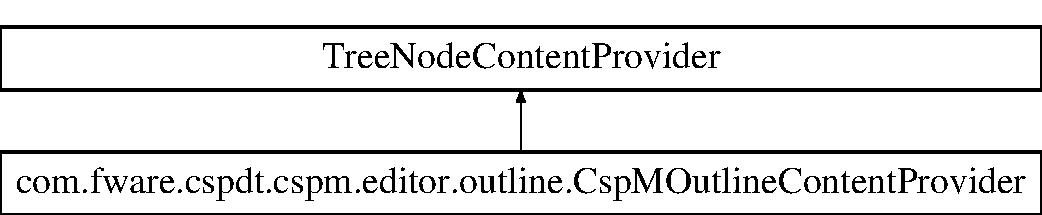
\includegraphics[height=2.000000cm]{classcom_1_1fware_1_1cspdt_1_1cspm_1_1editor_1_1outline_1_1_csp_m_outline_content_provider}
\end{center}
\end{figure}
\subsection*{Public Member Functions}
\begin{DoxyCompactItemize}
\item 
\mbox{\Hypertarget{classcom_1_1fware_1_1cspdt_1_1cspm_1_1editor_1_1outline_1_1_csp_m_outline_content_provider_a24495c72b973b36a711d1c270762b631}\label{classcom_1_1fware_1_1cspdt_1_1cspm_1_1editor_1_1outline_1_1_csp_m_outline_content_provider_a24495c72b973b36a711d1c270762b631}} 
{\bfseries Csp\+M\+Outline\+Content\+Provider} (\hyperlink{classcom_1_1fware_1_1cspdt_1_1cspm_1_1editor_1_1_csp_m_editor}{Csp\+M\+Editor} editor)
\item 
\mbox{\Hypertarget{classcom_1_1fware_1_1cspdt_1_1cspm_1_1editor_1_1outline_1_1_csp_m_outline_content_provider_aaba48556e6062d084b8c7d50203a5629}\label{classcom_1_1fware_1_1cspdt_1_1cspm_1_1editor_1_1outline_1_1_csp_m_outline_content_provider_aaba48556e6062d084b8c7d50203a5629}} 
void {\bfseries input\+Changed} (Viewer viewer, Object old\+Input, Object new\+Input)
\item 
\mbox{\Hypertarget{classcom_1_1fware_1_1cspdt_1_1cspm_1_1editor_1_1outline_1_1_csp_m_outline_content_provider_a66a9f9d7c76192a8327372a4cd7ed700}\label{classcom_1_1fware_1_1cspdt_1_1cspm_1_1editor_1_1outline_1_1_csp_m_outline_content_provider_a66a9f9d7c76192a8327372a4cd7ed700}} 
void {\bfseries dispose} ()
\item 
\mbox{\Hypertarget{classcom_1_1fware_1_1cspdt_1_1cspm_1_1editor_1_1outline_1_1_csp_m_outline_content_provider_ae7965511b8d03a8abe64a8daa0673a17}\label{classcom_1_1fware_1_1cspdt_1_1cspm_1_1editor_1_1outline_1_1_csp_m_outline_content_provider_ae7965511b8d03a8abe64a8daa0673a17}} 
boolean {\bfseries is\+Deleted} (Object element)
\item 
\mbox{\Hypertarget{classcom_1_1fware_1_1cspdt_1_1cspm_1_1editor_1_1outline_1_1_csp_m_outline_content_provider_a2080e54e6c292af2bf30778feb0f620f}\label{classcom_1_1fware_1_1cspdt_1_1cspm_1_1editor_1_1outline_1_1_csp_m_outline_content_provider_a2080e54e6c292af2bf30778feb0f620f}} 
Object \mbox{[}$\,$\mbox{]} {\bfseries get\+Elements} (Object element)
\item 
\mbox{\Hypertarget{classcom_1_1fware_1_1cspdt_1_1cspm_1_1editor_1_1outline_1_1_csp_m_outline_content_provider_ab87d115dc99422839b27f4f8b5daf3ea}\label{classcom_1_1fware_1_1cspdt_1_1cspm_1_1editor_1_1outline_1_1_csp_m_outline_content_provider_ab87d115dc99422839b27f4f8b5daf3ea}} 
boolean {\bfseries has\+Children} (Object element)
\item 
\mbox{\Hypertarget{classcom_1_1fware_1_1cspdt_1_1cspm_1_1editor_1_1outline_1_1_csp_m_outline_content_provider_a91364f3be9adb73d632450b9f3411925}\label{classcom_1_1fware_1_1cspdt_1_1cspm_1_1editor_1_1outline_1_1_csp_m_outline_content_provider_a91364f3be9adb73d632450b9f3411925}} 
Object {\bfseries get\+Parent} (Object element)
\item 
\mbox{\Hypertarget{classcom_1_1fware_1_1cspdt_1_1cspm_1_1editor_1_1outline_1_1_csp_m_outline_content_provider_ae355ce14693f49850ad590fcd290e540}\label{classcom_1_1fware_1_1cspdt_1_1cspm_1_1editor_1_1outline_1_1_csp_m_outline_content_provider_ae355ce14693f49850ad590fcd290e540}} 
Object \mbox{[}$\,$\mbox{]} {\bfseries get\+Children} (Object element)
\end{DoxyCompactItemize}
\subsection*{Protected Attributes}
\begin{DoxyCompactItemize}
\item 
\mbox{\Hypertarget{classcom_1_1fware_1_1cspdt_1_1cspm_1_1editor_1_1outline_1_1_csp_m_outline_content_provider_a1528f27271bb833b969a29939aa1a272}\label{classcom_1_1fware_1_1cspdt_1_1cspm_1_1editor_1_1outline_1_1_csp_m_outline_content_provider_a1528f27271bb833b969a29939aa1a272}} 
I\+Position\+Updater {\bfseries position\+Updater}
\item 
\mbox{\Hypertarget{classcom_1_1fware_1_1cspdt_1_1cspm_1_1editor_1_1outline_1_1_csp_m_outline_content_provider_af30280dee60b8750b67ecf03505d30b4}\label{classcom_1_1fware_1_1cspdt_1_1cspm_1_1editor_1_1outline_1_1_csp_m_outline_content_provider_af30280dee60b8750b67ecf03505d30b4}} 
Tree\+Node {\bfseries root\+Node}
\end{DoxyCompactItemize}
\subsection*{Static Protected Attributes}
\begin{DoxyCompactItemize}
\item 
\mbox{\Hypertarget{classcom_1_1fware_1_1cspdt_1_1cspm_1_1editor_1_1outline_1_1_csp_m_outline_content_provider_a32c1de6fd7411d0d03effa8d0bd56eef}\label{classcom_1_1fware_1_1cspdt_1_1cspm_1_1editor_1_1outline_1_1_csp_m_outline_content_provider_a32c1de6fd7411d0d03effa8d0bd56eef}} 
static final String {\bfseries S\+E\+G\+M\+E\+N\+TS} = \char`\"{}\+\_\+\+\_\+csp\+\_\+segments\char`\"{}
\end{DoxyCompactItemize}


\subsection{Detailed Description}
Esta classe e reponsavel por montar a estrutura da arvore que sera exibido na tela. 

\begin{DoxyAuthor}{Author}
A\+L\+V\+A\+RO, E\+V\+E\+R\+A\+L\+DA, F\+E\+L\+I\+PE, J\+O\+N\+A\+T\+H\+AN, J\+U\+V\+E\+N\+AL 
\end{DoxyAuthor}


The documentation for this class was generated from the following file\+:\begin{DoxyCompactItemize}
\item 
C\+:/\+Users/\+E\+V\+A/\+Downloads/eclipse/workspace/cspdt/com.\+fware.\+cspdt.\+cspm.\+editor/src/com/fware/cspdt/cspm/editor/outline/Csp\+M\+Outline\+Content\+Provider.\+java\end{DoxyCompactItemize}

\hypertarget{classcom_1_1fware_1_1cspdt_1_1cspm_1_1editor_1_1outline_1_1_csp_m_outline_tree_node}{}\section{com.\+fware.\+cspdt.\+cspm.\+editor.\+outline.\+Csp\+M\+Outline\+Tree\+Node Class Reference}
\label{classcom_1_1fware_1_1cspdt_1_1cspm_1_1editor_1_1outline_1_1_csp_m_outline_tree_node}\index{com.\+fware.\+cspdt.\+cspm.\+editor.\+outline.\+Csp\+M\+Outline\+Tree\+Node@{com.\+fware.\+cspdt.\+cspm.\+editor.\+outline.\+Csp\+M\+Outline\+Tree\+Node}}


Esta classe representa o no da arvore da classe Csp\+M\+Outline\+Tree\+Label\+Provider.  


Inheritance diagram for com.\+fware.\+cspdt.\+cspm.\+editor.\+outline.\+Csp\+M\+Outline\+Tree\+Node\+:\begin{figure}[H]
\begin{center}
\leavevmode
\includegraphics[height=2.000000cm]{classcom_1_1fware_1_1cspdt_1_1cspm_1_1editor_1_1outline_1_1_csp_m_outline_tree_node}
\end{center}
\end{figure}
\subsection*{Public Member Functions}
\begin{DoxyCompactItemize}
\item 
\mbox{\Hypertarget{classcom_1_1fware_1_1cspdt_1_1cspm_1_1editor_1_1outline_1_1_csp_m_outline_tree_node_ae906802314a97d4072e3a0121f001540}\label{classcom_1_1fware_1_1cspdt_1_1cspm_1_1editor_1_1outline_1_1_csp_m_outline_tree_node_ae906802314a97d4072e3a0121f001540}} 
{\bfseries Csp\+M\+Outline\+Tree\+Node} (Node node, Position position)
\item 
\mbox{\Hypertarget{classcom_1_1fware_1_1cspdt_1_1cspm_1_1editor_1_1outline_1_1_csp_m_outline_tree_node_a161f2d780e4ede63cf90f68eecb407bc}\label{classcom_1_1fware_1_1cspdt_1_1cspm_1_1editor_1_1outline_1_1_csp_m_outline_tree_node_a161f2d780e4ede63cf90f68eecb407bc}} 
void {\bfseries add\+Child} (\hyperlink{classcom_1_1fware_1_1cspdt_1_1cspm_1_1editor_1_1outline_1_1_csp_m_outline_tree_node}{Csp\+M\+Outline\+Tree\+Node} child)
\end{DoxyCompactItemize}
\subsection*{Public Attributes}
\begin{DoxyCompactItemize}
\item 
\mbox{\Hypertarget{classcom_1_1fware_1_1cspdt_1_1cspm_1_1editor_1_1outline_1_1_csp_m_outline_tree_node_a9f5d3f63d60f0c3d7df37ea321fc4f5b}\label{classcom_1_1fware_1_1cspdt_1_1cspm_1_1editor_1_1outline_1_1_csp_m_outline_tree_node_a9f5d3f63d60f0c3d7df37ea321fc4f5b}} 
final Position {\bfseries position}
\item 
\mbox{\Hypertarget{classcom_1_1fware_1_1cspdt_1_1cspm_1_1editor_1_1outline_1_1_csp_m_outline_tree_node_a4a1ec256a0b76c3143d1e86587303961}\label{classcom_1_1fware_1_1cspdt_1_1cspm_1_1editor_1_1outline_1_1_csp_m_outline_tree_node_a4a1ec256a0b76c3143d1e86587303961}} 
final List$<$ \hyperlink{classcom_1_1fware_1_1cspdt_1_1cspm_1_1editor_1_1outline_1_1_csp_m_outline_tree_node}{Csp\+M\+Outline\+Tree\+Node} $>$ {\bfseries children\+Backup}
\end{DoxyCompactItemize}


\subsection{Detailed Description}
Esta classe representa o no da arvore da classe Csp\+M\+Outline\+Tree\+Label\+Provider. 

\begin{DoxyAuthor}{Author}
A\+L\+V\+A\+RO, E\+V\+E\+R\+A\+L\+DA, F\+E\+L\+I\+PE, J\+O\+N\+A\+T\+H\+AN, J\+U\+V\+E\+N\+AL 
\end{DoxyAuthor}


The documentation for this class was generated from the following file\+:\begin{DoxyCompactItemize}
\item 
C\+:/\+Users/\+E\+V\+A/\+Downloads/eclipse/workspace/cspdt/com.\+fware.\+cspdt.\+cspm.\+editor/src/com/fware/cspdt/cspm/editor/outline/Csp\+M\+Outline\+Tree\+Node.\+java\end{DoxyCompactItemize}

\hypertarget{classcom_1_1fware_1_1cspdt_1_1cspm_1_1editor_1_1partition_1_1_csp_m_partitioner}{}\section{com.\+fware.\+cspdt.\+cspm.\+editor.\+partition.\+Csp\+M\+Partitioner Class Reference}
\label{classcom_1_1fware_1_1cspdt_1_1cspm_1_1editor_1_1partition_1_1_csp_m_partitioner}\index{com.\+fware.\+cspdt.\+cspm.\+editor.\+partition.\+Csp\+M\+Partitioner@{com.\+fware.\+cspdt.\+cspm.\+editor.\+partition.\+Csp\+M\+Partitioner}}


Classe que apresenta os recurso de particionamento do codigo C\+S\+PM.  


Inheritance diagram for com.\+fware.\+cspdt.\+cspm.\+editor.\+partition.\+Csp\+M\+Partitioner\+:\begin{figure}[H]
\begin{center}
\leavevmode
\includegraphics[height=2.000000cm]{classcom_1_1fware_1_1cspdt_1_1cspm_1_1editor_1_1partition_1_1_csp_m_partitioner}
\end{center}
\end{figure}


\subsection{Detailed Description}
Classe que apresenta os recurso de particionamento do codigo C\+S\+PM. 

\begin{DoxyAuthor}{Author}
A\+L\+V\+A\+RO, E\+V\+E\+R\+A\+L\+DA, F\+E\+L\+I\+PE, J\+O\+N\+A\+T\+H\+AN, J\+U\+V\+E\+N\+AL 
\end{DoxyAuthor}


The documentation for this class was generated from the following file\+:\begin{DoxyCompactItemize}
\item 
C\+:/\+Users/\+E\+V\+A/\+Downloads/eclipse/workspace/cspdt/com.\+fware.\+cspdt.\+cspm.\+editor/src/com/fware/cspdt/cspm/editor/partition/Csp\+M\+Partitioner.\+java\end{DoxyCompactItemize}

\hypertarget{classcom_1_1fware_1_1cspdt_1_1cspm_1_1editor_1_1partition_1_1_csp_m_partition_scanner}{}\section{com.\+fware.\+cspdt.\+cspm.\+editor.\+partition.\+Csp\+M\+Partition\+Scanner Class Reference}
\label{classcom_1_1fware_1_1cspdt_1_1cspm_1_1editor_1_1partition_1_1_csp_m_partition_scanner}\index{com.\+fware.\+cspdt.\+cspm.\+editor.\+partition.\+Csp\+M\+Partition\+Scanner@{com.\+fware.\+cspdt.\+cspm.\+editor.\+partition.\+Csp\+M\+Partition\+Scanner}}


Esta classe monta a estrategia de acao para realizar o escaneamento do documento por tokens e suas particoes.  


Inheritance diagram for com.\+fware.\+cspdt.\+cspm.\+editor.\+partition.\+Csp\+M\+Partition\+Scanner\+:\begin{figure}[H]
\begin{center}
\leavevmode
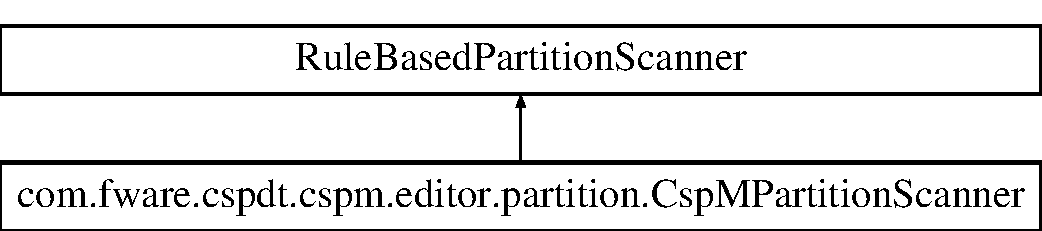
\includegraphics[height=2.000000cm]{classcom_1_1fware_1_1cspdt_1_1cspm_1_1editor_1_1partition_1_1_csp_m_partition_scanner}
\end{center}
\end{figure}
\subsection*{Static Public Attributes}
\begin{DoxyCompactItemize}
\item 
\mbox{\Hypertarget{classcom_1_1fware_1_1cspdt_1_1cspm_1_1editor_1_1partition_1_1_csp_m_partition_scanner_aa74e96b60b57ad569d7701af1cc216e1}\label{classcom_1_1fware_1_1cspdt_1_1cspm_1_1editor_1_1partition_1_1_csp_m_partition_scanner_aa74e96b60b57ad569d7701af1cc216e1}} 
static final String {\bfseries C\+S\+P\+M\+\_\+\+D\+E\+F\+A\+U\+L\+T\+\_\+\+C\+O\+N\+T\+E\+N\+T\+\_\+\+T\+Y\+PE} = I\+Document.\+D\+E\+F\+A\+U\+L\+T\+\_\+\+C\+O\+N\+T\+E\+N\+T\+\_\+\+T\+Y\+PE
\item 
\mbox{\Hypertarget{classcom_1_1fware_1_1cspdt_1_1cspm_1_1editor_1_1partition_1_1_csp_m_partition_scanner_a54db76e744688d692d1fd176dbf54eab}\label{classcom_1_1fware_1_1cspdt_1_1cspm_1_1editor_1_1partition_1_1_csp_m_partition_scanner_a54db76e744688d692d1fd176dbf54eab}} 
static final String {\bfseries C\+S\+P\+M\+\_\+\+C\+O\+M\+M\+E\+N\+T\+\_\+\+C\+O\+N\+T\+E\+N\+T\+\_\+\+T\+Y\+PE} = \char`\"{}\+\_\+\+\_\+csp\+\_\+comment\+\_\+content\+\_\+type\char`\"{}
\item 
\mbox{\Hypertarget{classcom_1_1fware_1_1cspdt_1_1cspm_1_1editor_1_1partition_1_1_csp_m_partition_scanner_ada9ada17754d6f358a8d5b82cb670f3c}\label{classcom_1_1fware_1_1cspdt_1_1cspm_1_1editor_1_1partition_1_1_csp_m_partition_scanner_ada9ada17754d6f358a8d5b82cb670f3c}} 
static final String {\bfseries C\+S\+P\+M\+\_\+\+M\+U\+L\+T\+I\+L\+I\+N\+E\+\_\+\+C\+O\+M\+M\+E\+N\+T\+\_\+\+C\+O\+N\+T\+E\+N\+T\+\_\+\+T\+Y\+PE} = \char`\"{}\+\_\+\+\_\+csp\+\_\+multicomment\+\_\+content\+\_\+type\char`\"{}
\item 
static final String \mbox{[}$\,$\mbox{]} {\bfseries P\+A\+R\+T\+I\+T\+I\+O\+N\+\_\+\+T\+Y\+P\+ES}
\end{DoxyCompactItemize}


\subsection{Detailed Description}
Esta classe monta a estrategia de acao para realizar o escaneamento do documento por tokens e suas particoes. 

\begin{DoxyAuthor}{Author}
A\+L\+V\+A\+RO, E\+V\+E\+R\+A\+L\+DA, F\+E\+L\+I\+PE, J\+O\+N\+A\+T\+H\+AN, J\+U\+V\+E\+N\+AL 
\end{DoxyAuthor}


\subsection{Member Data Documentation}
\mbox{\Hypertarget{classcom_1_1fware_1_1cspdt_1_1cspm_1_1editor_1_1partition_1_1_csp_m_partition_scanner_a0a05cab2396fe6da732c3deadd8c2500}\label{classcom_1_1fware_1_1cspdt_1_1cspm_1_1editor_1_1partition_1_1_csp_m_partition_scanner_a0a05cab2396fe6da732c3deadd8c2500}} 
\index{com\+::fware\+::cspdt\+::cspm\+::editor\+::partition\+::\+Csp\+M\+Partition\+Scanner@{com\+::fware\+::cspdt\+::cspm\+::editor\+::partition\+::\+Csp\+M\+Partition\+Scanner}!P\+A\+R\+T\+I\+T\+I\+O\+N\+\_\+\+T\+Y\+P\+ES@{P\+A\+R\+T\+I\+T\+I\+O\+N\+\_\+\+T\+Y\+P\+ES}}
\index{P\+A\+R\+T\+I\+T\+I\+O\+N\+\_\+\+T\+Y\+P\+ES@{P\+A\+R\+T\+I\+T\+I\+O\+N\+\_\+\+T\+Y\+P\+ES}!com\+::fware\+::cspdt\+::cspm\+::editor\+::partition\+::\+Csp\+M\+Partition\+Scanner@{com\+::fware\+::cspdt\+::cspm\+::editor\+::partition\+::\+Csp\+M\+Partition\+Scanner}}
\subsubsection{\texorpdfstring{P\+A\+R\+T\+I\+T\+I\+O\+N\+\_\+\+T\+Y\+P\+ES}{PARTITION\_TYPES}}
{\footnotesize\ttfamily final String \mbox{[}$\,$\mbox{]} com.\+fware.\+cspdt.\+cspm.\+editor.\+partition.\+Csp\+M\+Partition\+Scanner.\+P\+A\+R\+T\+I\+T\+I\+O\+N\+\_\+\+T\+Y\+P\+ES\hspace{0.3cm}{\ttfamily [static]}}

{\bfseries Initial value\+:}
\begin{DoxyCode}
= \textcolor{keyword}{new} String[] \{ 
            CSPM\_DEFAULT\_CONTENT\_TYPE, 
            CSPM\_COMMENT\_CONTENT\_TYPE,
            CSPM\_MULTILINE\_COMMENT\_CONTENT\_TYPE \}
\end{DoxyCode}


The documentation for this class was generated from the following file\+:\begin{DoxyCompactItemize}
\item 
C\+:/\+Users/\+E\+V\+A/\+Downloads/eclipse/workspace/cspdt/com.\+fware.\+cspdt.\+cspm.\+editor/src/com/fware/cspdt/cspm/editor/partition/Csp\+M\+Partition\+Scanner.\+java\end{DoxyCompactItemize}

\hypertarget{classcom_1_1fware_1_1cspdt_1_1cspm_1_1editor_1_1config_1_1_csp_m_process_completion_processor}{}\section{com.\+fware.\+cspdt.\+cspm.\+editor.\+config.\+Csp\+M\+Process\+Completion\+Processor Class Reference}
\label{classcom_1_1fware_1_1cspdt_1_1cspm_1_1editor_1_1config_1_1_csp_m_process_completion_processor}\index{com.\+fware.\+cspdt.\+cspm.\+editor.\+config.\+Csp\+M\+Process\+Completion\+Processor@{com.\+fware.\+cspdt.\+cspm.\+editor.\+config.\+Csp\+M\+Process\+Completion\+Processor}}


Esta classe define as acoes de auto complete.  


Inheritance diagram for com.\+fware.\+cspdt.\+cspm.\+editor.\+config.\+Csp\+M\+Process\+Completion\+Processor\+:\begin{figure}[H]
\begin{center}
\leavevmode
\includegraphics[height=2.000000cm]{classcom_1_1fware_1_1cspdt_1_1cspm_1_1editor_1_1config_1_1_csp_m_process_completion_processor}
\end{center}
\end{figure}
\subsection*{Classes}
\begin{DoxyCompactItemize}
\item 
class {\bfseries Keywords\+Comparator}
\begin{DoxyCompactList}\small\item\em Classe reponsavel pela comparacao de propostas. \end{DoxyCompactList}\end{DoxyCompactItemize}
\subsection*{Public Member Functions}
\begin{DoxyCompactItemize}
\item 
\mbox{\Hypertarget{classcom_1_1fware_1_1cspdt_1_1cspm_1_1editor_1_1config_1_1_csp_m_process_completion_processor_a06f6b7e4ce46fbb8ea109eb8e3e3c973}\label{classcom_1_1fware_1_1cspdt_1_1cspm_1_1editor_1_1config_1_1_csp_m_process_completion_processor_a06f6b7e4ce46fbb8ea109eb8e3e3c973}} 
{\bfseries Csp\+M\+Process\+Completion\+Processor} (\hyperlink{classcom_1_1fware_1_1cspdt_1_1cspm_1_1editor_1_1_csp_m_editor}{Csp\+M\+Editor} editor)
\item 
\mbox{\Hypertarget{classcom_1_1fware_1_1cspdt_1_1cspm_1_1editor_1_1config_1_1_csp_m_process_completion_processor_a92f2e4e1f8cb6585cd7d779bceb4afbe}\label{classcom_1_1fware_1_1cspdt_1_1cspm_1_1editor_1_1config_1_1_csp_m_process_completion_processor_a92f2e4e1f8cb6585cd7d779bceb4afbe}} 
I\+Completion\+Proposal \mbox{[}$\,$\mbox{]} \hyperlink{classcom_1_1fware_1_1cspdt_1_1cspm_1_1editor_1_1config_1_1_csp_m_process_completion_processor_a92f2e4e1f8cb6585cd7d779bceb4afbe}{compute\+Completion\+Proposals} (I\+Text\+Viewer viewer, int offset)
\begin{DoxyCompactList}\small\item\em Este metodo e o responsavel por fornecer o conjunto de sugestoes de acordo com a posicao do cursor. \end{DoxyCompactList}\item 
\mbox{\Hypertarget{classcom_1_1fware_1_1cspdt_1_1cspm_1_1editor_1_1config_1_1_csp_m_process_completion_processor_aeb2234d9b3f0ba22cfb09220352218de}\label{classcom_1_1fware_1_1cspdt_1_1cspm_1_1editor_1_1config_1_1_csp_m_process_completion_processor_aeb2234d9b3f0ba22cfb09220352218de}} 
I\+Context\+Information \mbox{[}$\,$\mbox{]} {\bfseries compute\+Context\+Information} (I\+Text\+Viewer viewer, int offset)
\item 
\mbox{\Hypertarget{classcom_1_1fware_1_1cspdt_1_1cspm_1_1editor_1_1config_1_1_csp_m_process_completion_processor_a3a7bfa456d6fbaf9e9e71fa9cd6c8f6e}\label{classcom_1_1fware_1_1cspdt_1_1cspm_1_1editor_1_1config_1_1_csp_m_process_completion_processor_a3a7bfa456d6fbaf9e9e71fa9cd6c8f6e}} 
char \mbox{[}$\,$\mbox{]} {\bfseries get\+Completion\+Proposal\+Auto\+Activation\+Characters} ()
\item 
\mbox{\Hypertarget{classcom_1_1fware_1_1cspdt_1_1cspm_1_1editor_1_1config_1_1_csp_m_process_completion_processor_a04c78632c12d2fa79b9986b7a45e5530}\label{classcom_1_1fware_1_1cspdt_1_1cspm_1_1editor_1_1config_1_1_csp_m_process_completion_processor_a04c78632c12d2fa79b9986b7a45e5530}} 
char \mbox{[}$\,$\mbox{]} {\bfseries get\+Context\+Information\+Auto\+Activation\+Characters} ()
\item 
\mbox{\Hypertarget{classcom_1_1fware_1_1cspdt_1_1cspm_1_1editor_1_1config_1_1_csp_m_process_completion_processor_af9a6c3c1da9d2de7726bd9f3802ff05b}\label{classcom_1_1fware_1_1cspdt_1_1cspm_1_1editor_1_1config_1_1_csp_m_process_completion_processor_af9a6c3c1da9d2de7726bd9f3802ff05b}} 
String {\bfseries get\+Error\+Message} ()
\item 
\mbox{\Hypertarget{classcom_1_1fware_1_1cspdt_1_1cspm_1_1editor_1_1config_1_1_csp_m_process_completion_processor_ae564757118503ad570ea14fed78988c3}\label{classcom_1_1fware_1_1cspdt_1_1cspm_1_1editor_1_1config_1_1_csp_m_process_completion_processor_ae564757118503ad570ea14fed78988c3}} 
I\+Context\+Information\+Validator {\bfseries get\+Context\+Information\+Validator} ()
\end{DoxyCompactItemize}


\subsection{Detailed Description}
Esta classe define as acoes de auto complete. 

\begin{DoxyAuthor}{Author}
A\+L\+V\+A\+RO, E\+V\+E\+R\+A\+L\+DA, F\+E\+L\+I\+PE, J\+O\+N\+A\+T\+H\+AN, J\+U\+V\+E\+N\+AL 
\end{DoxyAuthor}


The documentation for this class was generated from the following file\+:\begin{DoxyCompactItemize}
\item 
C\+:/\+Users/\+E\+V\+A/\+Downloads/eclipse/workspace/cspdt/com.\+fware.\+cspdt.\+cspm.\+editor/src/com/fware/cspdt/cspm/editor/config/Csp\+M\+Process\+Completion\+Processor.\+java\end{DoxyCompactItemize}

\hypertarget{classcom_1_1fware_1_1cspdt_1_1cspm_1_1editor_1_1project_1_1_csp_m_project}{}\section{com.\+fware.\+cspdt.\+cspm.\+editor.\+project.\+Csp\+M\+Project Class Reference}
\label{classcom_1_1fware_1_1cspdt_1_1cspm_1_1editor_1_1project_1_1_csp_m_project}\index{com.\+fware.\+cspdt.\+cspm.\+editor.\+project.\+Csp\+M\+Project@{com.\+fware.\+cspdt.\+cspm.\+editor.\+project.\+Csp\+M\+Project}}


This class represents a project.  


\subsection*{Public Member Functions}
\begin{DoxyCompactItemize}
\item 
\mbox{\Hypertarget{classcom_1_1fware_1_1cspdt_1_1cspm_1_1editor_1_1project_1_1_csp_m_project_a45336c1eaf6d37004c11c412400002f8}\label{classcom_1_1fware_1_1cspdt_1_1cspm_1_1editor_1_1project_1_1_csp_m_project_a45336c1eaf6d37004c11c412400002f8}} 
String {\bfseries get\+Project\+Name} ()
\item 
\mbox{\Hypertarget{classcom_1_1fware_1_1cspdt_1_1cspm_1_1editor_1_1project_1_1_csp_m_project_a7feb904f4cde7bfe23856260db455e08}\label{classcom_1_1fware_1_1cspdt_1_1cspm_1_1editor_1_1project_1_1_csp_m_project_a7feb904f4cde7bfe23856260db455e08}} 
void {\bfseries set\+Project\+Name} (String project\+Name)
\item 
\mbox{\Hypertarget{classcom_1_1fware_1_1cspdt_1_1cspm_1_1editor_1_1project_1_1_csp_m_project_a19ccc9901718986790658df43880f341}\label{classcom_1_1fware_1_1cspdt_1_1cspm_1_1editor_1_1project_1_1_csp_m_project_a19ccc9901718986790658df43880f341}} 
List {\bfseries get\+Source\+Dirs} ()
\item 
\mbox{\Hypertarget{classcom_1_1fware_1_1cspdt_1_1cspm_1_1editor_1_1project_1_1_csp_m_project_af323a55d16ea1cd83938f9b0add938a5}\label{classcom_1_1fware_1_1cspdt_1_1cspm_1_1editor_1_1project_1_1_csp_m_project_af323a55d16ea1cd83938f9b0add938a5}} 
void {\bfseries set\+Source\+Dirs} (List source\+Dirs)
\item 
\mbox{\Hypertarget{classcom_1_1fware_1_1cspdt_1_1cspm_1_1editor_1_1project_1_1_csp_m_project_aaeb4dbff3712ec64465d88d3c225fcc5}\label{classcom_1_1fware_1_1cspdt_1_1cspm_1_1editor_1_1project_1_1_csp_m_project_aaeb4dbff3712ec64465d88d3c225fcc5}} 
String {\bfseries get\+Project\+Location} ()
\item 
\mbox{\Hypertarget{classcom_1_1fware_1_1cspdt_1_1cspm_1_1editor_1_1project_1_1_csp_m_project_a2827f8079eddd54cafe06a849b7fa766}\label{classcom_1_1fware_1_1cspdt_1_1cspm_1_1editor_1_1project_1_1_csp_m_project_a2827f8079eddd54cafe06a849b7fa766}} 
void {\bfseries set\+Project\+Location} (String text)
\item 
\mbox{\Hypertarget{classcom_1_1fware_1_1cspdt_1_1cspm_1_1editor_1_1project_1_1_csp_m_project_ab2cdbeb693949ff5da63aa663e9cff41}\label{classcom_1_1fware_1_1cspdt_1_1cspm_1_1editor_1_1project_1_1_csp_m_project_ab2cdbeb693949ff5da63aa663e9cff41}} 
String {\bfseries get\+Main\+Source\+File\+Name} ()
\item 
\mbox{\Hypertarget{classcom_1_1fware_1_1cspdt_1_1cspm_1_1editor_1_1project_1_1_csp_m_project_adf190f65ee0ff4bdc35e7dc9245bc57a}\label{classcom_1_1fware_1_1cspdt_1_1cspm_1_1editor_1_1project_1_1_csp_m_project_adf190f65ee0ff4bdc35e7dc9245bc57a}} 
void {\bfseries set\+Main\+Source\+File\+Name} (String source\+File)
\item 
\mbox{\Hypertarget{classcom_1_1fware_1_1cspdt_1_1cspm_1_1editor_1_1project_1_1_csp_m_project_a20016dc081d8ba33e4c709118f42290f}\label{classcom_1_1fware_1_1cspdt_1_1cspm_1_1editor_1_1project_1_1_csp_m_project_a20016dc081d8ba33e4c709118f42290f}} 
String {\bfseries get\+Output\+Dir} ()
\item 
\mbox{\Hypertarget{classcom_1_1fware_1_1cspdt_1_1cspm_1_1editor_1_1project_1_1_csp_m_project_a2663911be9648bbc28a3930666182cff}\label{classcom_1_1fware_1_1cspdt_1_1cspm_1_1editor_1_1project_1_1_csp_m_project_a2663911be9648bbc28a3930666182cff}} 
void {\bfseries set\+Output\+Dir} (String output\+Dir)
\end{DoxyCompactItemize}


\subsection{Detailed Description}
This class represents a project. 

It contains all the values that a project has. These values can be changed in the new project wizard.

\begin{DoxyAuthor}{Author}
Joabe Jesus 
\end{DoxyAuthor}


The documentation for this class was generated from the following file\+:\begin{DoxyCompactItemize}
\item 
C\+:/\+Users/\+E\+V\+A/\+Downloads/eclipse/workspace/cspdt/com.\+fware.\+cspdt.\+cspm.\+editor/src/com/fware/cspdt/cspm/editor/project/Csp\+M\+Project.\+java\end{DoxyCompactItemize}

\hypertarget{classcom_1_1fware_1_1cspdt_1_1cspm_1_1editor_1_1project_1_1_csp_m_project_properties}{}\section{com.\+fware.\+cspdt.\+cspm.\+editor.\+project.\+Csp\+M\+Project\+Properties Class Reference}
\label{classcom_1_1fware_1_1cspdt_1_1cspm_1_1editor_1_1project_1_1_csp_m_project_properties}\index{com.\+fware.\+cspdt.\+cspm.\+editor.\+project.\+Csp\+M\+Project\+Properties@{com.\+fware.\+cspdt.\+cspm.\+editor.\+project.\+Csp\+M\+Project\+Properties}}


Esta classe define propriedades de um projeto C\+S\+PM.  


\subsection*{Static Public Attributes}
\begin{DoxyCompactItemize}
\item 
\mbox{\Hypertarget{classcom_1_1fware_1_1cspdt_1_1cspm_1_1editor_1_1project_1_1_csp_m_project_properties_a0158c0d2b534b25ab11c3d2a51483cde}\label{classcom_1_1fware_1_1cspdt_1_1cspm_1_1editor_1_1project_1_1_csp_m_project_properties_a0158c0d2b534b25ab11c3d2a51483cde}} 
static final String {\bfseries C\+S\+P\+\_\+\+P\+R\+O\+J\+E\+C\+T\+\_\+\+S\+E\+T\+T\+I\+N\+G\+S\+\_\+\+F\+I\+LE} = \char`\"{}.cspproject\char`\"{}
\end{DoxyCompactItemize}


\subsection{Detailed Description}
Esta classe define propriedades de um projeto C\+S\+PM. 

\begin{DoxyAuthor}{Author}
A\+L\+V\+A\+RO, E\+V\+E\+R\+A\+L\+DA, F\+E\+L\+I\+PE, J\+O\+N\+A\+T\+H\+AN, J\+U\+V\+E\+N\+AL 
\end{DoxyAuthor}


The documentation for this class was generated from the following file\+:\begin{DoxyCompactItemize}
\item 
C\+:/\+Users/\+E\+V\+A/\+Downloads/eclipse/workspace/cspdt/com.\+fware.\+cspdt.\+cspm.\+editor/src/com/fware/cspdt/cspm/editor/project/Csp\+M\+Project\+Properties.\+java\end{DoxyCompactItemize}

\hypertarget{classcom_1_1fware_1_1cspdt_1_1cspm_1_1editor_1_1config_1_1_csp_m_reconciling_strategy}{}\section{com.\+fware.\+cspdt.\+cspm.\+editor.\+config.\+Csp\+M\+Reconciling\+Strategy Class Reference}
\label{classcom_1_1fware_1_1cspdt_1_1cspm_1_1editor_1_1config_1_1_csp_m_reconciling_strategy}\index{com.\+fware.\+cspdt.\+cspm.\+editor.\+config.\+Csp\+M\+Reconciling\+Strategy@{com.\+fware.\+cspdt.\+cspm.\+editor.\+config.\+Csp\+M\+Reconciling\+Strategy}}


Esta classe cria uma estrategia de acao para a representacao do texto na presenca de mudancas no codigo C\+S\+PM.  


Inheritance diagram for com.\+fware.\+cspdt.\+cspm.\+editor.\+config.\+Csp\+M\+Reconciling\+Strategy\+:\begin{figure}[H]
\begin{center}
\leavevmode
\includegraphics[height=2.000000cm]{classcom_1_1fware_1_1cspdt_1_1cspm_1_1editor_1_1config_1_1_csp_m_reconciling_strategy}
\end{center}
\end{figure}
\subsection*{Public Member Functions}
\begin{DoxyCompactItemize}
\item 
\mbox{\Hypertarget{classcom_1_1fware_1_1cspdt_1_1cspm_1_1editor_1_1config_1_1_csp_m_reconciling_strategy_a35bf14074f25f727296be20ab8010cd6}\label{classcom_1_1fware_1_1cspdt_1_1cspm_1_1editor_1_1config_1_1_csp_m_reconciling_strategy_a35bf14074f25f727296be20ab8010cd6}} 
{\bfseries Csp\+M\+Reconciling\+Strategy} (\hyperlink{classcom_1_1fware_1_1cspdt_1_1cspm_1_1editor_1_1_csp_m_editor}{Csp\+M\+Editor} editor)
\item 
\mbox{\Hypertarget{classcom_1_1fware_1_1cspdt_1_1cspm_1_1editor_1_1config_1_1_csp_m_reconciling_strategy_a87671e3d5dff3a07593d019cc9e245e2}\label{classcom_1_1fware_1_1cspdt_1_1cspm_1_1editor_1_1config_1_1_csp_m_reconciling_strategy_a87671e3d5dff3a07593d019cc9e245e2}} 
\hyperlink{classcom_1_1fware_1_1cspdt_1_1cspm_1_1editor_1_1_csp_m_editor}{Csp\+M\+Editor} {\bfseries get\+Editor} ()
\item 
\mbox{\Hypertarget{classcom_1_1fware_1_1cspdt_1_1cspm_1_1editor_1_1config_1_1_csp_m_reconciling_strategy_a267f60e0239f81a1e437a5e764a57095}\label{classcom_1_1fware_1_1cspdt_1_1cspm_1_1editor_1_1config_1_1_csp_m_reconciling_strategy_a267f60e0239f81a1e437a5e764a57095}} 
void \hyperlink{classcom_1_1fware_1_1cspdt_1_1cspm_1_1editor_1_1config_1_1_csp_m_reconciling_strategy_a267f60e0239f81a1e437a5e764a57095}{initial\+Reconcile} ()
\begin{DoxyCompactList}\small\item\em Verifica inicio e fim da mudanca no texto. \end{DoxyCompactList}\item 
\mbox{\Hypertarget{classcom_1_1fware_1_1cspdt_1_1cspm_1_1editor_1_1config_1_1_csp_m_reconciling_strategy_a6663cb7417bfabd1fd01f464643cc78c}\label{classcom_1_1fware_1_1cspdt_1_1cspm_1_1editor_1_1config_1_1_csp_m_reconciling_strategy_a6663cb7417bfabd1fd01f464643cc78c}} 
void {\bfseries set\+Document} (I\+Document document)
\item 
\mbox{\Hypertarget{classcom_1_1fware_1_1cspdt_1_1cspm_1_1editor_1_1config_1_1_csp_m_reconciling_strategy_aac7acad99cc16f8a73a17f8df51a1f33}\label{classcom_1_1fware_1_1cspdt_1_1cspm_1_1editor_1_1config_1_1_csp_m_reconciling_strategy_aac7acad99cc16f8a73a17f8df51a1f33}} 
void {\bfseries reconcile} (Dirty\+Region arg0, I\+Region arg1)
\item 
\mbox{\Hypertarget{classcom_1_1fware_1_1cspdt_1_1cspm_1_1editor_1_1config_1_1_csp_m_reconciling_strategy_a08c2583e9e001d367c0e30f5208d6904}\label{classcom_1_1fware_1_1cspdt_1_1cspm_1_1editor_1_1config_1_1_csp_m_reconciling_strategy_a08c2583e9e001d367c0e30f5208d6904}} 
void {\bfseries reconcile} (I\+Region arg0)
\end{DoxyCompactItemize}
\subsection*{Protected Attributes}
\begin{DoxyCompactItemize}
\item 
\mbox{\Hypertarget{classcom_1_1fware_1_1cspdt_1_1cspm_1_1editor_1_1config_1_1_csp_m_reconciling_strategy_a32d28514e5f49b442eb48dfa3657abae}\label{classcom_1_1fware_1_1cspdt_1_1cspm_1_1editor_1_1config_1_1_csp_m_reconciling_strategy_a32d28514e5f49b442eb48dfa3657abae}} 
final List$<$ Position $>$ \hyperlink{classcom_1_1fware_1_1cspdt_1_1cspm_1_1editor_1_1config_1_1_csp_m_reconciling_strategy_a32d28514e5f49b442eb48dfa3657abae}{f\+Positions} = new Array\+List$<$Position$>$()
\begin{DoxyCompactList}\small\item\em holds the calculated positions \end{DoxyCompactList}\item 
\mbox{\Hypertarget{classcom_1_1fware_1_1cspdt_1_1cspm_1_1editor_1_1config_1_1_csp_m_reconciling_strategy_afa451850691ae557a816cc5bd5d76d1a}\label{classcom_1_1fware_1_1cspdt_1_1cspm_1_1editor_1_1config_1_1_csp_m_reconciling_strategy_afa451850691ae557a816cc5bd5d76d1a}} 
int \hyperlink{classcom_1_1fware_1_1cspdt_1_1cspm_1_1editor_1_1config_1_1_csp_m_reconciling_strategy_afa451850691ae557a816cc5bd5d76d1a}{f\+Offset}
\begin{DoxyCompactList}\small\item\em The offset of the next character to be read. \end{DoxyCompactList}\item 
\mbox{\Hypertarget{classcom_1_1fware_1_1cspdt_1_1cspm_1_1editor_1_1config_1_1_csp_m_reconciling_strategy_af52adef988902c51cc4054d2ad46911a}\label{classcom_1_1fware_1_1cspdt_1_1cspm_1_1editor_1_1config_1_1_csp_m_reconciling_strategy_af52adef988902c51cc4054d2ad46911a}} 
int \hyperlink{classcom_1_1fware_1_1cspdt_1_1cspm_1_1editor_1_1config_1_1_csp_m_reconciling_strategy_af52adef988902c51cc4054d2ad46911a}{f\+Range\+End}
\begin{DoxyCompactList}\small\item\em The end offset of the range to be scanned. \end{DoxyCompactList}\end{DoxyCompactItemize}


\subsection{Detailed Description}
Esta classe cria uma estrategia de acao para a representacao do texto na presenca de mudancas no codigo C\+S\+PM. 

\begin{DoxyAuthor}{Author}
A\+L\+V\+A\+RO, E\+V\+E\+R\+A\+L\+DA, F\+E\+L\+I\+PE, J\+O\+N\+A\+T\+H\+AN, J\+U\+V\+E\+N\+AL 
\end{DoxyAuthor}


The documentation for this class was generated from the following file\+:\begin{DoxyCompactItemize}
\item 
C\+:/\+Users/\+E\+V\+A/\+Downloads/eclipse/workspace/cspdt/com.\+fware.\+cspdt.\+cspm.\+editor/src/com/fware/cspdt/cspm/editor/config/Csp\+M\+Reconciling\+Strategy.\+java\end{DoxyCompactItemize}

\hypertarget{classcom_1_1fware_1_1cspdt_1_1cspm_1_1editor_1_1link_1_1_csp_m_ref_extractor}{}\section{com.\+fware.\+cspdt.\+cspm.\+editor.\+link.\+Csp\+M\+Ref\+Extractor Class Reference}
\label{classcom_1_1fware_1_1cspdt_1_1cspm_1_1editor_1_1link_1_1_csp_m_ref_extractor}\index{com.\+fware.\+cspdt.\+cspm.\+editor.\+link.\+Csp\+M\+Ref\+Extractor@{com.\+fware.\+cspdt.\+cspm.\+editor.\+link.\+Csp\+M\+Ref\+Extractor}}


Esta classe pretende distinguir as referencias pelos tipos da linguagem C\+S\+PM.  


Inheritance diagram for com.\+fware.\+cspdt.\+cspm.\+editor.\+link.\+Csp\+M\+Ref\+Extractor\+:\begin{figure}[H]
\begin{center}
\leavevmode
\includegraphics[height=2.000000cm]{classcom_1_1fware_1_1cspdt_1_1cspm_1_1editor_1_1link_1_1_csp_m_ref_extractor}
\end{center}
\end{figure}
\subsection*{Public Member Functions}
\begin{DoxyCompactItemize}
\item 
\mbox{\Hypertarget{classcom_1_1fware_1_1cspdt_1_1cspm_1_1editor_1_1link_1_1_csp_m_ref_extractor_ae58fb5ca1456f9544bb8a6c071c9e04f}\label{classcom_1_1fware_1_1cspdt_1_1cspm_1_1editor_1_1link_1_1_csp_m_ref_extractor_ae58fb5ca1456f9544bb8a6c071c9e04f}} 
{\bfseries Csp\+M\+Ref\+Extractor} (I\+Document document, Csp\+M\+Model info)
\item 
\mbox{\Hypertarget{classcom_1_1fware_1_1cspdt_1_1cspm_1_1editor_1_1link_1_1_csp_m_ref_extractor_a6ece0e48a01c155d31a735db53b5a91e}\label{classcom_1_1fware_1_1cspdt_1_1cspm_1_1editor_1_1link_1_1_csp_m_ref_extractor_a6ece0e48a01c155d31a735db53b5a91e}} 
void {\bfseries in\+A\+Csp\+Specification} (A\+Csp\+Specification node)
\item 
\mbox{\Hypertarget{classcom_1_1fware_1_1cspdt_1_1cspm_1_1editor_1_1link_1_1_csp_m_ref_extractor_a24fd458e5d42fb8ad3d27ce8cb7cbb07}\label{classcom_1_1fware_1_1cspdt_1_1cspm_1_1editor_1_1link_1_1_csp_m_ref_extractor_a24fd458e5d42fb8ad3d27ce8cb7cbb07}} 
void {\bfseries out\+A\+Csp\+Specification} (A\+Csp\+Specification node)
\item 
\mbox{\Hypertarget{classcom_1_1fware_1_1cspdt_1_1cspm_1_1editor_1_1link_1_1_csp_m_ref_extractor_ab7250e61a1e0c8896d9e851f67707a06}\label{classcom_1_1fware_1_1cspdt_1_1cspm_1_1editor_1_1link_1_1_csp_m_ref_extractor_ab7250e61a1e0c8896d9e851f67707a06}} 
void {\bfseries in\+A\+Csp\+Definition\+Paragraph} (A\+Csp\+Definition\+Paragraph node)
\item 
\mbox{\Hypertarget{classcom_1_1fware_1_1cspdt_1_1cspm_1_1editor_1_1link_1_1_csp_m_ref_extractor_a0e0d89d39cd33ebee10cf94257b77899}\label{classcom_1_1fware_1_1cspdt_1_1cspm_1_1editor_1_1link_1_1_csp_m_ref_extractor_a0e0d89d39cd33ebee10cf94257b77899}} 
void {\bfseries out\+A\+Csp\+Definition\+Paragraph} (A\+Csp\+Definition\+Paragraph node)
\item 
\mbox{\Hypertarget{classcom_1_1fware_1_1cspdt_1_1cspm_1_1editor_1_1link_1_1_csp_m_ref_extractor_aa8276d6728fe96b937506039e29355bb}\label{classcom_1_1fware_1_1cspdt_1_1cspm_1_1editor_1_1link_1_1_csp_m_ref_extractor_aa8276d6728fe96b937506039e29355bb}} 
void {\bfseries case\+A\+Csp\+Definition\+Paragraph} (A\+Csp\+Definition\+Paragraph node)
\item 
\mbox{\Hypertarget{classcom_1_1fware_1_1cspdt_1_1cspm_1_1editor_1_1link_1_1_csp_m_ref_extractor_a6188009230e8fef43ee4d9ee1da296a7}\label{classcom_1_1fware_1_1cspdt_1_1cspm_1_1editor_1_1link_1_1_csp_m_ref_extractor_a6188009230e8fef43ee4d9ee1da296a7}} 
void {\bfseries case\+A\+Csp\+Function\+Definition} (A\+Csp\+Function\+Definition node)
\item 
\mbox{\Hypertarget{classcom_1_1fware_1_1cspdt_1_1cspm_1_1editor_1_1link_1_1_csp_m_ref_extractor_a3e04876b4ff6a84bf1549d414c4f811b}\label{classcom_1_1fware_1_1cspdt_1_1cspm_1_1editor_1_1link_1_1_csp_m_ref_extractor_a3e04876b4ff6a84bf1549d414c4f811b}} 
void {\bfseries case\+A\+Csp\+Constant\+Definition} (A\+Csp\+Constant\+Definition node)
\item 
\mbox{\Hypertarget{classcom_1_1fware_1_1cspdt_1_1cspm_1_1editor_1_1link_1_1_csp_m_ref_extractor_ac5df3aebe9bfdf654f5bbe7a58ef2daa}\label{classcom_1_1fware_1_1cspdt_1_1cspm_1_1editor_1_1link_1_1_csp_m_ref_extractor_ac5df3aebe9bfdf654f5bbe7a58ef2daa}} 
void {\bfseries case\+A\+Csp\+Datatype\+Definition} (A\+Csp\+Datatype\+Definition node)
\item 
\mbox{\Hypertarget{classcom_1_1fware_1_1cspdt_1_1cspm_1_1editor_1_1link_1_1_csp_m_ref_extractor_ab4cd63c2f081633c391d96f49016604f}\label{classcom_1_1fware_1_1cspdt_1_1cspm_1_1editor_1_1link_1_1_csp_m_ref_extractor_ab4cd63c2f081633c391d96f49016604f}} 
void {\bfseries case\+A\+Csp\+Subtype\+Definition} (A\+Csp\+Subtype\+Definition node)
\item 
\mbox{\Hypertarget{classcom_1_1fware_1_1cspdt_1_1cspm_1_1editor_1_1link_1_1_csp_m_ref_extractor_a31116fbe8881f1e99f1ea08179d5868e}\label{classcom_1_1fware_1_1cspdt_1_1cspm_1_1editor_1_1link_1_1_csp_m_ref_extractor_a31116fbe8881f1e99f1ea08179d5868e}} 
void {\bfseries case\+A\+Csp\+Nametype\+Definition} (A\+Csp\+Nametype\+Definition node)
\item 
\mbox{\Hypertarget{classcom_1_1fware_1_1cspdt_1_1cspm_1_1editor_1_1link_1_1_csp_m_ref_extractor_ad302fc4e0eeb6440ac7339dcf7c34798}\label{classcom_1_1fware_1_1cspdt_1_1cspm_1_1editor_1_1link_1_1_csp_m_ref_extractor_ad302fc4e0eeb6440ac7339dcf7c34798}} 
void {\bfseries case\+A\+Csp\+Process\+Definition} (A\+Csp\+Process\+Definition node)
\item 
\mbox{\Hypertarget{classcom_1_1fware_1_1cspdt_1_1cspm_1_1editor_1_1link_1_1_csp_m_ref_extractor_af9cd43f7ce99e36e3e7c3401ac4a7099}\label{classcom_1_1fware_1_1cspdt_1_1cspm_1_1editor_1_1link_1_1_csp_m_ref_extractor_af9cd43f7ce99e36e3e7c3401ac4a7099}} 
void {\bfseries case\+A\+Csp\+Abstract\+Definition} (A\+Csp\+Abstract\+Definition node)
\item 
\mbox{\Hypertarget{classcom_1_1fware_1_1cspdt_1_1cspm_1_1editor_1_1link_1_1_csp_m_ref_extractor_a683f22dd9d20a5c9ef0b9fd823ece5f6}\label{classcom_1_1fware_1_1cspdt_1_1cspm_1_1editor_1_1link_1_1_csp_m_ref_extractor_a683f22dd9d20a5c9ef0b9fd823ece5f6}} 
void {\bfseries case\+A\+Csp\+Channel} (A\+Csp\+Channel node)
\end{DoxyCompactItemize}


\subsection{Detailed Description}
Esta classe pretende distinguir as referencias pelos tipos da linguagem C\+S\+PM. 

\begin{DoxyAuthor}{Author}
A\+L\+V\+A\+RO, E\+V\+E\+R\+A\+L\+DA, F\+E\+L\+I\+PE, J\+O\+N\+A\+T\+H\+AN, J\+U\+V\+E\+N\+AL 
\end{DoxyAuthor}


The documentation for this class was generated from the following file\+:\begin{DoxyCompactItemize}
\item 
C\+:/\+Users/\+E\+V\+A/\+Downloads/eclipse/workspace/cspdt/com.\+fware.\+cspdt.\+cspm.\+editor/src/com/fware/cspdt/cspm/editor/link/Csp\+M\+Ref\+Extractor.\+java\end{DoxyCompactItemize}

\hypertarget{classcom_1_1fware_1_1cspdt_1_1cspm_1_1editor_1_1scanner_1_1_csp_m_scanner}{}\section{com.\+fware.\+cspdt.\+cspm.\+editor.\+scanner.\+Csp\+M\+Scanner Class Reference}
\label{classcom_1_1fware_1_1cspdt_1_1cspm_1_1editor_1_1scanner_1_1_csp_m_scanner}\index{com.\+fware.\+cspdt.\+cspm.\+editor.\+scanner.\+Csp\+M\+Scanner@{com.\+fware.\+cspdt.\+cspm.\+editor.\+scanner.\+Csp\+M\+Scanner}}


Nesta classe sao definidas as palavras chaves do C\+S\+PM.  


Inheritance diagram for com.\+fware.\+cspdt.\+cspm.\+editor.\+scanner.\+Csp\+M\+Scanner\+:\begin{figure}[H]
\begin{center}
\leavevmode
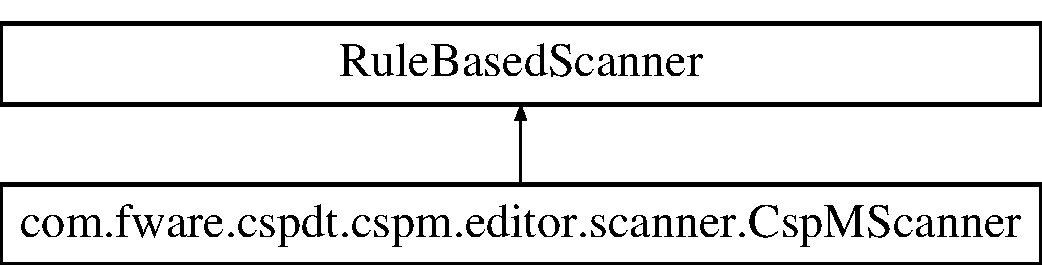
\includegraphics[height=2.000000cm]{classcom_1_1fware_1_1cspdt_1_1cspm_1_1editor_1_1scanner_1_1_csp_m_scanner}
\end{center}
\end{figure}
\subsection*{Public Member Functions}
\begin{DoxyCompactItemize}
\item 
\mbox{\Hypertarget{classcom_1_1fware_1_1cspdt_1_1cspm_1_1editor_1_1scanner_1_1_csp_m_scanner_a22c6a3b72a8aac91999fc67ea878f562}\label{classcom_1_1fware_1_1cspdt_1_1cspm_1_1editor_1_1scanner_1_1_csp_m_scanner_a22c6a3b72a8aac91999fc67ea878f562}} 
{\bfseries Csp\+M\+Scanner} (\hyperlink{classcom_1_1fware_1_1cspdt_1_1cspm_1_1editor_1_1config_1_1_csp_m_color_manager}{Csp\+M\+Color\+Manager} color\+Manager)
\item 
void \hyperlink{classcom_1_1fware_1_1cspdt_1_1cspm_1_1editor_1_1scanner_1_1_csp_m_scanner_af76db62b0ad376ba6d53325a76f7a9e7}{add\+Process} (String process\+Name)
\begin{DoxyCompactList}\small\item\em Classe responsavel por adicionar um nome de processo, definido em codigo ao conjunto de tokens conhecidos. \end{DoxyCompactList}\end{DoxyCompactItemize}


\subsection{Detailed Description}
Nesta classe sao definidas as palavras chaves do C\+S\+PM. 

\begin{DoxyAuthor}{Author}
A\+L\+V\+A\+RO, E\+V\+E\+R\+A\+L\+DA, F\+E\+L\+I\+PE, J\+O\+N\+A\+T\+H\+AN, J\+U\+V\+E\+N\+AL 
\end{DoxyAuthor}


\subsection{Member Function Documentation}
\mbox{\Hypertarget{classcom_1_1fware_1_1cspdt_1_1cspm_1_1editor_1_1scanner_1_1_csp_m_scanner_af76db62b0ad376ba6d53325a76f7a9e7}\label{classcom_1_1fware_1_1cspdt_1_1cspm_1_1editor_1_1scanner_1_1_csp_m_scanner_af76db62b0ad376ba6d53325a76f7a9e7}} 
\index{com\+::fware\+::cspdt\+::cspm\+::editor\+::scanner\+::\+Csp\+M\+Scanner@{com\+::fware\+::cspdt\+::cspm\+::editor\+::scanner\+::\+Csp\+M\+Scanner}!add\+Process@{add\+Process}}
\index{add\+Process@{add\+Process}!com\+::fware\+::cspdt\+::cspm\+::editor\+::scanner\+::\+Csp\+M\+Scanner@{com\+::fware\+::cspdt\+::cspm\+::editor\+::scanner\+::\+Csp\+M\+Scanner}}
\subsubsection{\texorpdfstring{add\+Process()}{addProcess()}}
{\footnotesize\ttfamily void com.\+fware.\+cspdt.\+cspm.\+editor.\+scanner.\+Csp\+M\+Scanner.\+add\+Process (\begin{DoxyParamCaption}\item[{String}]{process\+Name }\end{DoxyParamCaption})\hspace{0.3cm}{\ttfamily [inline]}}



Classe responsavel por adicionar um nome de processo, definido em codigo ao conjunto de tokens conhecidos. 


\begin{DoxyParams}{Parameters}
{\em process\+Name} & \\
\hline
\end{DoxyParams}


The documentation for this class was generated from the following file\+:\begin{DoxyCompactItemize}
\item 
C\+:/\+Users/\+E\+V\+A/\+Downloads/eclipse/workspace/cspdt/com.\+fware.\+cspdt.\+cspm.\+editor/src/com/fware/cspdt/cspm/editor/scanner/Csp\+M\+Scanner.\+java\end{DoxyCompactItemize}

\hypertarget{classcom_1_1fware_1_1cspdt_1_1cspm_1_1editor_1_1config_1_1_csp_m_source_viewer_configuration}{}\section{com.\+fware.\+cspdt.\+cspm.\+editor.\+config.\+Csp\+M\+Source\+Viewer\+Configuration Class Reference}
\label{classcom_1_1fware_1_1cspdt_1_1cspm_1_1editor_1_1config_1_1_csp_m_source_viewer_configuration}\index{com.\+fware.\+cspdt.\+cspm.\+editor.\+config.\+Csp\+M\+Source\+Viewer\+Configuration@{com.\+fware.\+cspdt.\+cspm.\+editor.\+config.\+Csp\+M\+Source\+Viewer\+Configuration}}


Nesta classe s�o definidas as configuracoes de vizualizacao do codigo.  


Inheritance diagram for com.\+fware.\+cspdt.\+cspm.\+editor.\+config.\+Csp\+M\+Source\+Viewer\+Configuration\+:\begin{figure}[H]
\begin{center}
\leavevmode
\includegraphics[height=2.000000cm]{classcom_1_1fware_1_1cspdt_1_1cspm_1_1editor_1_1config_1_1_csp_m_source_viewer_configuration}
\end{center}
\end{figure}
\subsection*{Public Member Functions}
\begin{DoxyCompactItemize}
\item 
\mbox{\Hypertarget{classcom_1_1fware_1_1cspdt_1_1cspm_1_1editor_1_1config_1_1_csp_m_source_viewer_configuration_a6272fff4f7e9e531f622eb830870cc46}\label{classcom_1_1fware_1_1cspdt_1_1cspm_1_1editor_1_1config_1_1_csp_m_source_viewer_configuration_a6272fff4f7e9e531f622eb830870cc46}} 
{\bfseries Csp\+M\+Source\+Viewer\+Configuration} (\hyperlink{classcom_1_1fware_1_1cspdt_1_1cspm_1_1editor_1_1_csp_m_editor}{Csp\+M\+Editor} editor, \hyperlink{classcom_1_1fware_1_1cspdt_1_1cspm_1_1editor_1_1config_1_1_csp_m_color_manager}{Csp\+M\+Color\+Manager} color\+Manager)
\item 
\mbox{\Hypertarget{classcom_1_1fware_1_1cspdt_1_1cspm_1_1editor_1_1config_1_1_csp_m_source_viewer_configuration_a00816f87b69a14bb8ba0d0e42b4a9295}\label{classcom_1_1fware_1_1cspdt_1_1cspm_1_1editor_1_1config_1_1_csp_m_source_viewer_configuration_a00816f87b69a14bb8ba0d0e42b4a9295}} 
String \mbox{[}$\,$\mbox{]} {\bfseries get\+Configured\+Content\+Types} (I\+Source\+Viewer source\+Viewer)
\item 
\mbox{\Hypertarget{classcom_1_1fware_1_1cspdt_1_1cspm_1_1editor_1_1config_1_1_csp_m_source_viewer_configuration_a7fd57be4fdc8452bebad0c38587d92c3}\label{classcom_1_1fware_1_1cspdt_1_1cspm_1_1editor_1_1config_1_1_csp_m_source_viewer_configuration_a7fd57be4fdc8452bebad0c38587d92c3}} 
I\+Reconciler {\bfseries get\+Reconciler} (I\+Source\+Viewer source\+Viewer)
\item 
\mbox{\Hypertarget{classcom_1_1fware_1_1cspdt_1_1cspm_1_1editor_1_1config_1_1_csp_m_source_viewer_configuration_a633e2f3b880e2c8d135ef5db637c4d77}\label{classcom_1_1fware_1_1cspdt_1_1cspm_1_1editor_1_1config_1_1_csp_m_source_viewer_configuration_a633e2f3b880e2c8d135ef5db637c4d77}} 
I\+Presentation\+Reconciler {\bfseries get\+Presentation\+Reconciler} (I\+Source\+Viewer source\+Viewer)
\item 
\mbox{\Hypertarget{classcom_1_1fware_1_1cspdt_1_1cspm_1_1editor_1_1config_1_1_csp_m_source_viewer_configuration_a51378a59b25f3a39129cd4cdc445698b}\label{classcom_1_1fware_1_1cspdt_1_1cspm_1_1editor_1_1config_1_1_csp_m_source_viewer_configuration_a51378a59b25f3a39129cd4cdc445698b}} 
Color {\bfseries get\+Prefered\+Color} (I\+Preference\+Store prefs, String id)
\item 
\mbox{\Hypertarget{classcom_1_1fware_1_1cspdt_1_1cspm_1_1editor_1_1config_1_1_csp_m_source_viewer_configuration_a3838e0274664968d1ace5927479292e4}\label{classcom_1_1fware_1_1cspdt_1_1cspm_1_1editor_1_1config_1_1_csp_m_source_viewer_configuration_a3838e0274664968d1ace5927479292e4}} 
I\+Text\+Double\+Click\+Strategy {\bfseries get\+Double\+Click\+Strategy} (I\+Source\+Viewer source\+Viewer, String content\+Type)
\item 
\mbox{\Hypertarget{classcom_1_1fware_1_1cspdt_1_1cspm_1_1editor_1_1config_1_1_csp_m_source_viewer_configuration_a626233f50842c9ca4af53decd3ea1832}\label{classcom_1_1fware_1_1cspdt_1_1cspm_1_1editor_1_1config_1_1_csp_m_source_viewer_configuration_a626233f50842c9ca4af53decd3ea1832}} 
I\+Auto\+Edit\+Strategy \mbox{[}$\,$\mbox{]} {\bfseries get\+Auto\+Edit\+Strategies} (I\+Source\+Viewer source\+Viewer, String content\+Type)
\item 
\mbox{\Hypertarget{classcom_1_1fware_1_1cspdt_1_1cspm_1_1editor_1_1config_1_1_csp_m_source_viewer_configuration_a659c48945f82bbf9dc78011da4554981}\label{classcom_1_1fware_1_1cspdt_1_1cspm_1_1editor_1_1config_1_1_csp_m_source_viewer_configuration_a659c48945f82bbf9dc78011da4554981}} 
I\+Content\+Assistant {\bfseries get\+Content\+Assistant} (I\+Source\+Viewer source\+Viewer)
\item 
\mbox{\Hypertarget{classcom_1_1fware_1_1cspdt_1_1cspm_1_1editor_1_1config_1_1_csp_m_source_viewer_configuration_a0d98703c70d20f67e4bd2a4a35ca6244}\label{classcom_1_1fware_1_1cspdt_1_1cspm_1_1editor_1_1config_1_1_csp_m_source_viewer_configuration_a0d98703c70d20f67e4bd2a4a35ca6244}} 
\hyperlink{classcom_1_1fware_1_1cspdt_1_1cspm_1_1editor_1_1link_1_1_csp_m_hyperlink_detector}{Csp\+M\+Hyperlink\+Detector} \mbox{[}$\,$\mbox{]} {\bfseries get\+Hyperlink\+Detectors} (I\+Source\+Viewer source\+Viewer)
\item 
\mbox{\Hypertarget{classcom_1_1fware_1_1cspdt_1_1cspm_1_1editor_1_1config_1_1_csp_m_source_viewer_configuration_a0dd49b63076fb9600b8c9fae719106a5}\label{classcom_1_1fware_1_1cspdt_1_1cspm_1_1editor_1_1config_1_1_csp_m_source_viewer_configuration_a0dd49b63076fb9600b8c9fae719106a5}} 
\hyperlink{classcom_1_1fware_1_1cspdt_1_1cspm_1_1editor_1_1link_1_1_csp_m_hyperlink_presenter}{Csp\+M\+Hyperlink\+Presenter} {\bfseries get\+Hyperlink\+Presenter} (I\+Source\+Viewer source\+Viewer)
\end{DoxyCompactItemize}
\subsection*{Protected Member Functions}
\begin{DoxyCompactItemize}
\item 
\mbox{\Hypertarget{classcom_1_1fware_1_1cspdt_1_1cspm_1_1editor_1_1config_1_1_csp_m_source_viewer_configuration_ab12a907b0128987c194e4bd1b7b3365b}\label{classcom_1_1fware_1_1cspdt_1_1cspm_1_1editor_1_1config_1_1_csp_m_source_viewer_configuration_ab12a907b0128987c194e4bd1b7b3365b}} 
\hyperlink{classcom_1_1fware_1_1cspdt_1_1cspm_1_1editor_1_1scanner_1_1_csp_m_scanner}{Csp\+M\+Scanner} {\bfseries get\+Scanner} ()
\end{DoxyCompactItemize}


\subsection{Detailed Description}
Nesta classe s�o definidas as configuracoes de vizualizacao do codigo. 

Ela quarda configuracoes do auto complete, sintax highlight entre outros.

\begin{DoxyAuthor}{Author}
A\+L\+V\+A\+RO, E\+V\+E\+R\+A\+L\+DA, F\+E\+L\+I\+PE, J\+O\+N\+A\+T\+H\+AN, J\+U\+V\+E\+N\+AL 
\end{DoxyAuthor}


The documentation for this class was generated from the following file\+:\begin{DoxyCompactItemize}
\item 
C\+:/\+Users/\+E\+V\+A/\+Downloads/eclipse/workspace/cspdt/com.\+fware.\+cspdt.\+cspm.\+editor/src/com/fware/cspdt/cspm/editor/config/Csp\+M\+Source\+Viewer\+Configuration.\+java\end{DoxyCompactItemize}

\hypertarget{classcom_1_1fware_1_1cspdt_1_1cspm_1_1editor_1_1hover_1_1_csp_m_text_hover}{}\section{com.\+fware.\+cspdt.\+cspm.\+editor.\+hover.\+Csp\+M\+Text\+Hover Class Reference}
\label{classcom_1_1fware_1_1cspdt_1_1cspm_1_1editor_1_1hover_1_1_csp_m_text_hover}\index{com.\+fware.\+cspdt.\+cspm.\+editor.\+hover.\+Csp\+M\+Text\+Hover@{com.\+fware.\+cspdt.\+cspm.\+editor.\+hover.\+Csp\+M\+Text\+Hover}}


Esta classe define a estrategia de acao para quando o mouse passa sobre o texto no codigo C\+S\+PM.  


Inheritance diagram for com.\+fware.\+cspdt.\+cspm.\+editor.\+hover.\+Csp\+M\+Text\+Hover\+:\begin{figure}[H]
\begin{center}
\leavevmode
\includegraphics[height=2.000000cm]{classcom_1_1fware_1_1cspdt_1_1cspm_1_1editor_1_1hover_1_1_csp_m_text_hover}
\end{center}
\end{figure}
\subsection*{Public Member Functions}
\begin{DoxyCompactItemize}
\item 
\mbox{\Hypertarget{classcom_1_1fware_1_1cspdt_1_1cspm_1_1editor_1_1hover_1_1_csp_m_text_hover_aec291b826826f0cb61db572130f95cbd}\label{classcom_1_1fware_1_1cspdt_1_1cspm_1_1editor_1_1hover_1_1_csp_m_text_hover_aec291b826826f0cb61db572130f95cbd}} 
I\+Region {\bfseries get\+Hover\+Region} (I\+Text\+Viewer text\+Viewer, int offset)
\item 
\mbox{\Hypertarget{classcom_1_1fware_1_1cspdt_1_1cspm_1_1editor_1_1hover_1_1_csp_m_text_hover_a23fed69af0b24aa640b81bc3b5edfe69}\label{classcom_1_1fware_1_1cspdt_1_1cspm_1_1editor_1_1hover_1_1_csp_m_text_hover_a23fed69af0b24aa640b81bc3b5edfe69}} 
String {\bfseries get\+Hover\+Info} (I\+Text\+Viewer text\+Viewer, I\+Region hover\+Region)
\end{DoxyCompactItemize}


\subsection{Detailed Description}
Esta classe define a estrategia de acao para quando o mouse passa sobre o texto no codigo C\+S\+PM. 

\begin{DoxyAuthor}{Author}
A\+L\+V\+A\+RO, E\+V\+E\+R\+A\+L\+DA, F\+E\+L\+I\+PE, J\+O\+N\+A\+T\+H\+AN, J\+U\+V\+E\+N\+AL 
\end{DoxyAuthor}


The documentation for this class was generated from the following file\+:\begin{DoxyCompactItemize}
\item 
C\+:/\+Users/\+E\+V\+A/\+Downloads/eclipse/workspace/cspdt/com.\+fware.\+cspdt.\+cspm.\+editor/src/com/fware/cspdt/cspm/editor/hover/Csp\+M\+Text\+Hover.\+java\end{DoxyCompactItemize}

\hypertarget{classcom_1_1fware_1_1cspdt_1_1cspm_1_1editor_1_1scanner_1_1_csp_whitespace_detector}{}\section{com.\+fware.\+cspdt.\+cspm.\+editor.\+scanner.\+Csp\+Whitespace\+Detector Class Reference}
\label{classcom_1_1fware_1_1cspdt_1_1cspm_1_1editor_1_1scanner_1_1_csp_whitespace_detector}\index{com.\+fware.\+cspdt.\+cspm.\+editor.\+scanner.\+Csp\+Whitespace\+Detector@{com.\+fware.\+cspdt.\+cspm.\+editor.\+scanner.\+Csp\+Whitespace\+Detector}}
Inheritance diagram for com.\+fware.\+cspdt.\+cspm.\+editor.\+scanner.\+Csp\+Whitespace\+Detector\+:\begin{figure}[H]
\begin{center}
\leavevmode
\includegraphics[height=2.000000cm]{classcom_1_1fware_1_1cspdt_1_1cspm_1_1editor_1_1scanner_1_1_csp_whitespace_detector}
\end{center}
\end{figure}
\subsection*{Public Member Functions}
\begin{DoxyCompactItemize}
\item 
boolean \hyperlink{classcom_1_1fware_1_1cspdt_1_1cspm_1_1editor_1_1scanner_1_1_csp_whitespace_detector_ab058042f9f83da533d3a355f718c0a57}{is\+Whitespace} (char c)
\begin{DoxyCompactList}\small\item\em Detects is the given character a white space character. \end{DoxyCompactList}\end{DoxyCompactItemize}


\subsection{Member Function Documentation}
\mbox{\Hypertarget{classcom_1_1fware_1_1cspdt_1_1cspm_1_1editor_1_1scanner_1_1_csp_whitespace_detector_ab058042f9f83da533d3a355f718c0a57}\label{classcom_1_1fware_1_1cspdt_1_1cspm_1_1editor_1_1scanner_1_1_csp_whitespace_detector_ab058042f9f83da533d3a355f718c0a57}} 
\index{com\+::fware\+::cspdt\+::cspm\+::editor\+::scanner\+::\+Csp\+Whitespace\+Detector@{com\+::fware\+::cspdt\+::cspm\+::editor\+::scanner\+::\+Csp\+Whitespace\+Detector}!is\+Whitespace@{is\+Whitespace}}
\index{is\+Whitespace@{is\+Whitespace}!com\+::fware\+::cspdt\+::cspm\+::editor\+::scanner\+::\+Csp\+Whitespace\+Detector@{com\+::fware\+::cspdt\+::cspm\+::editor\+::scanner\+::\+Csp\+Whitespace\+Detector}}
\subsubsection{\texorpdfstring{is\+Whitespace()}{isWhitespace()}}
{\footnotesize\ttfamily boolean com.\+fware.\+cspdt.\+cspm.\+editor.\+scanner.\+Csp\+Whitespace\+Detector.\+is\+Whitespace (\begin{DoxyParamCaption}\item[{char}]{c }\end{DoxyParamCaption})\hspace{0.3cm}{\ttfamily [inline]}}



Detects is the given character a white space character. 


\begin{DoxyParams}{Parameters}
{\em c} & A character to test.\\
\hline
\end{DoxyParams}
\begin{DoxyReturn}{Returns}
{\ttfamily true} if the character is a white space character, {\ttfamily false} otherwise.
\end{DoxyReturn}
\begin{DoxySeeAlso}{See also}
org.\+eclipse.\+jface.\+text.\+rules.\+I\+Whitespace\+Detector\+::is\+Whitespace(char) 
\end{DoxySeeAlso}


The documentation for this class was generated from the following file\+:\begin{DoxyCompactItemize}
\item 
C\+:/\+Users/\+E\+V\+A/\+Downloads/eclipse/workspace/cspdt/com.\+fware.\+cspdt.\+cspm.\+editor/src/com/fware/cspdt/cspm/editor/scanner/Csp\+Whitespace\+Detector.\+java\end{DoxyCompactItemize}

\hypertarget{enumcom_1_1fware_1_1cspdt_1_1cspm_1_1editor_1_1config_1_1_keywords}{}\section{com.\+fware.\+cspdt.\+cspm.\+editor.\+config.\+Keywords Enum Reference}
\label{enumcom_1_1fware_1_1cspdt_1_1cspm_1_1editor_1_1config_1_1_keywords}\index{com.\+fware.\+cspdt.\+cspm.\+editor.\+config.\+Keywords@{com.\+fware.\+cspdt.\+cspm.\+editor.\+config.\+Keywords}}


Esta classe e uma enumeracao com as palavras reservadas do C\+S\+PM.  


\subsection*{Public Member Functions}
\begin{DoxyCompactItemize}
\item 
\mbox{\Hypertarget{enumcom_1_1fware_1_1cspdt_1_1cspm_1_1editor_1_1config_1_1_keywords_a9773a880667143eaffa32d850f887b15}\label{enumcom_1_1fware_1_1cspdt_1_1cspm_1_1editor_1_1config_1_1_keywords_a9773a880667143eaffa32d850f887b15}} 
{\bfseries Keywords} (String v)
\item 
\mbox{\Hypertarget{enumcom_1_1fware_1_1cspdt_1_1cspm_1_1editor_1_1config_1_1_keywords_afa5f52efa871dcff12de993e917d6e00}\label{enumcom_1_1fware_1_1cspdt_1_1cspm_1_1editor_1_1config_1_1_keywords_afa5f52efa871dcff12de993e917d6e00}} 
String {\bfseries get\+Value} ()
\end{DoxyCompactItemize}
\subsection*{Public Attributes}
\begin{DoxyCompactItemize}
\item 
\mbox{\Hypertarget{enumcom_1_1fware_1_1cspdt_1_1cspm_1_1editor_1_1config_1_1_keywords_a2c456bded9dd8ee043a9272356a94892}\label{enumcom_1_1fware_1_1cspdt_1_1cspm_1_1editor_1_1config_1_1_keywords_a2c456bded9dd8ee043a9272356a94892}} 
{\bfseries I\+N\+C\+L\+U\+DE} =(\char`\"{}include\char`\"{})
\item 
\mbox{\Hypertarget{enumcom_1_1fware_1_1cspdt_1_1cspm_1_1editor_1_1config_1_1_keywords_a46361ff65ad886414ebeb67abfdaf519}\label{enumcom_1_1fware_1_1cspdt_1_1cspm_1_1editor_1_1config_1_1_keywords_a46361ff65ad886414ebeb67abfdaf519}} 
{\bfseries T\+R\+A\+N\+S\+P\+A\+R\+E\+NT} =(\char`\"{}transparent\char`\"{})
\item 
\mbox{\Hypertarget{enumcom_1_1fware_1_1cspdt_1_1cspm_1_1editor_1_1config_1_1_keywords_a0284a0397d7a5d19fc65487ee8b193c6}\label{enumcom_1_1fware_1_1cspdt_1_1cspm_1_1editor_1_1config_1_1_keywords_a0284a0397d7a5d19fc65487ee8b193c6}} 
{\bfseries E\+X\+T\+E\+R\+N\+AL} =(\char`\"{}external\char`\"{})
\item 
\mbox{\Hypertarget{enumcom_1_1fware_1_1cspdt_1_1cspm_1_1editor_1_1config_1_1_keywords_a7905802641aa42d9cd9e827d1a0f88f5}\label{enumcom_1_1fware_1_1cspdt_1_1cspm_1_1editor_1_1config_1_1_keywords_a7905802641aa42d9cd9e827d1a0f88f5}} 
{\bfseries D\+A\+T\+A\+T\+Y\+PE} =(\char`\"{}datatype\char`\"{})
\item 
\mbox{\Hypertarget{enumcom_1_1fware_1_1cspdt_1_1cspm_1_1editor_1_1config_1_1_keywords_ad9c9c433d6d052b93b560b2a9a550894}\label{enumcom_1_1fware_1_1cspdt_1_1cspm_1_1editor_1_1config_1_1_keywords_ad9c9c433d6d052b93b560b2a9a550894}} 
{\bfseries S\+U\+B\+T\+Y\+PE} =(\char`\"{}subtype\char`\"{})
\item 
\mbox{\Hypertarget{enumcom_1_1fware_1_1cspdt_1_1cspm_1_1editor_1_1config_1_1_keywords_a3fbb736b0a313d943b90161768101235}\label{enumcom_1_1fware_1_1cspdt_1_1cspm_1_1editor_1_1config_1_1_keywords_a3fbb736b0a313d943b90161768101235}} 
{\bfseries N\+A\+M\+E\+T\+Y\+PE} =(\char`\"{}nametype\char`\"{})
\item 
\mbox{\Hypertarget{enumcom_1_1fware_1_1cspdt_1_1cspm_1_1editor_1_1config_1_1_keywords_adca02c203a5722f80073696ae33eb508}\label{enumcom_1_1fware_1_1cspdt_1_1cspm_1_1editor_1_1config_1_1_keywords_adca02c203a5722f80073696ae33eb508}} 
{\bfseries M\+O\+D\+U\+LE} =(\char`\"{}module\char`\"{})
\item 
\mbox{\Hypertarget{enumcom_1_1fware_1_1cspdt_1_1cspm_1_1editor_1_1config_1_1_keywords_af5ae824359dd95fd4de0035253344429}\label{enumcom_1_1fware_1_1cspdt_1_1cspm_1_1editor_1_1config_1_1_keywords_af5ae824359dd95fd4de0035253344429}} 
{\bfseries E\+X\+P\+O\+R\+TS} =(\char`\"{}exports\char`\"{})
\item 
\mbox{\Hypertarget{enumcom_1_1fware_1_1cspdt_1_1cspm_1_1editor_1_1config_1_1_keywords_a2f1efac057e9052be71c73ed33921f9a}\label{enumcom_1_1fware_1_1cspdt_1_1cspm_1_1editor_1_1config_1_1_keywords_a2f1efac057e9052be71c73ed33921f9a}} 
{\bfseries E\+N\+D\+M\+O\+D\+U\+LE} =(\char`\"{}endmodule\char`\"{})
\item 
\mbox{\Hypertarget{enumcom_1_1fware_1_1cspdt_1_1cspm_1_1editor_1_1config_1_1_keywords_a95cd7315345473fb9a489a907bb769a5}\label{enumcom_1_1fware_1_1cspdt_1_1cspm_1_1editor_1_1config_1_1_keywords_a95cd7315345473fb9a489a907bb769a5}} 
{\bfseries I\+N\+S\+T\+A\+N\+CE} =(\char`\"{}instance\char`\"{})
\item 
\mbox{\Hypertarget{enumcom_1_1fware_1_1cspdt_1_1cspm_1_1editor_1_1config_1_1_keywords_ada0ca7803950df67136d82bbe9a285d0}\label{enumcom_1_1fware_1_1cspdt_1_1cspm_1_1editor_1_1config_1_1_keywords_ada0ca7803950df67136d82bbe9a285d0}} 
{\bfseries C\+H\+A\+N\+N\+EL} =(\char`\"{}channel\char`\"{})
\item 
\mbox{\Hypertarget{enumcom_1_1fware_1_1cspdt_1_1cspm_1_1editor_1_1config_1_1_keywords_a0dae7ea5c8cd69b27b9988c665ab1c2c}\label{enumcom_1_1fware_1_1cspdt_1_1cspm_1_1editor_1_1config_1_1_keywords_a0dae7ea5c8cd69b27b9988c665ab1c2c}} 
{\bfseries IF} =(\char`\"{}if\char`\"{})
\item 
\mbox{\Hypertarget{enumcom_1_1fware_1_1cspdt_1_1cspm_1_1editor_1_1config_1_1_keywords_a46ab7fee7d8a9565c42b7b35aca08327}\label{enumcom_1_1fware_1_1cspdt_1_1cspm_1_1editor_1_1config_1_1_keywords_a46ab7fee7d8a9565c42b7b35aca08327}} 
{\bfseries T\+H\+EN} =(\char`\"{}then\char`\"{})
\item 
\mbox{\Hypertarget{enumcom_1_1fware_1_1cspdt_1_1cspm_1_1editor_1_1config_1_1_keywords_a4bc0c93b2ceb5351f2782e05cc9d0811}\label{enumcom_1_1fware_1_1cspdt_1_1cspm_1_1editor_1_1config_1_1_keywords_a4bc0c93b2ceb5351f2782e05cc9d0811}} 
{\bfseries E\+L\+SE} =(\char`\"{}else\char`\"{})
\item 
\mbox{\Hypertarget{enumcom_1_1fware_1_1cspdt_1_1cspm_1_1editor_1_1config_1_1_keywords_ae9a6a387d117c3128de0503a40cbe8b6}\label{enumcom_1_1fware_1_1cspdt_1_1cspm_1_1editor_1_1config_1_1_keywords_ae9a6a387d117c3128de0503a40cbe8b6}} 
{\bfseries L\+ET} =(\char`\"{}left\char`\"{})
\item 
\mbox{\Hypertarget{enumcom_1_1fware_1_1cspdt_1_1cspm_1_1editor_1_1config_1_1_keywords_a9a9d91848c3ac1c5167186c4b0478b78}\label{enumcom_1_1fware_1_1cspdt_1_1cspm_1_1editor_1_1config_1_1_keywords_a9a9d91848c3ac1c5167186c4b0478b78}} 
{\bfseries W\+I\+T\+H\+IN} =(\char`\"{}within\char`\"{})
\item 
\mbox{\Hypertarget{enumcom_1_1fware_1_1cspdt_1_1cspm_1_1editor_1_1config_1_1_keywords_acc916ea95813d42d83057eff6a926294}\label{enumcom_1_1fware_1_1cspdt_1_1cspm_1_1editor_1_1config_1_1_keywords_acc916ea95813d42d83057eff6a926294}} 
{\bfseries T\+R\+UE} =(\char`\"{}true\char`\"{})
\item 
\mbox{\Hypertarget{enumcom_1_1fware_1_1cspdt_1_1cspm_1_1editor_1_1config_1_1_keywords_ab0d4358a3cdc7b63c2ba01bd8a80f4cc}\label{enumcom_1_1fware_1_1cspdt_1_1cspm_1_1editor_1_1config_1_1_keywords_ab0d4358a3cdc7b63c2ba01bd8a80f4cc}} 
{\bfseries F\+A\+L\+SE} =(\char`\"{}false\char`\"{})
\item 
\mbox{\Hypertarget{enumcom_1_1fware_1_1cspdt_1_1cspm_1_1editor_1_1config_1_1_keywords_abc0f2cf4fa932fbccb28cdc1b2e8036c}\label{enumcom_1_1fware_1_1cspdt_1_1cspm_1_1editor_1_1config_1_1_keywords_abc0f2cf4fa932fbccb28cdc1b2e8036c}} 
{\bfseries A\+S\+S\+E\+RT} =(\char`\"{}assert\char`\"{})
\item 
\mbox{\Hypertarget{enumcom_1_1fware_1_1cspdt_1_1cspm_1_1editor_1_1config_1_1_keywords_a289b1aeb390232eb6e39535001468fd7}\label{enumcom_1_1fware_1_1cspdt_1_1cspm_1_1editor_1_1config_1_1_keywords_a289b1aeb390232eb6e39535001468fd7}} 
{\bfseries P\+R\+I\+NT} =(\char`\"{}print\char`\"{})
\item 
\mbox{\Hypertarget{enumcom_1_1fware_1_1cspdt_1_1cspm_1_1editor_1_1config_1_1_keywords_a323949d719e8a10d107cb709282152ef}\label{enumcom_1_1fware_1_1cspdt_1_1cspm_1_1editor_1_1config_1_1_keywords_a323949d719e8a10d107cb709282152ef}} 
String {\bfseries value}
\end{DoxyCompactItemize}


\subsection{Detailed Description}
Esta classe e uma enumeracao com as palavras reservadas do C\+S\+PM. 

\begin{DoxyAuthor}{Author}
A\+L\+V\+A\+RO, E\+V\+E\+R\+A\+L\+DA, F\+E\+L\+I\+PE, J\+O\+N\+A\+T\+H\+AN, J\+U\+V\+E\+N\+AL 
\end{DoxyAuthor}


The documentation for this enum was generated from the following file\+:\begin{DoxyCompactItemize}
\item 
C\+:/\+Users/\+E\+V\+A/\+Downloads/eclipse/workspace/cspdt/com.\+fware.\+cspdt.\+cspm.\+editor/src/com/fware/cspdt/cspm/editor/config/Keywords.\+java\end{DoxyCompactItemize}

\hypertarget{classcom_1_1fware_1_1cspdt_1_1cspm_1_1editor_1_1config_1_1_non_rule_based_damager_repairer}{}\section{com.\+fware.\+cspdt.\+cspm.\+editor.\+config.\+Non\+Rule\+Based\+Damager\+Repairer Class Reference}
\label{classcom_1_1fware_1_1cspdt_1_1cspm_1_1editor_1_1config_1_1_non_rule_based_damager_repairer}\index{com.\+fware.\+cspdt.\+cspm.\+editor.\+config.\+Non\+Rule\+Based\+Damager\+Repairer@{com.\+fware.\+cspdt.\+cspm.\+editor.\+config.\+Non\+Rule\+Based\+Damager\+Repairer}}


Esta classe e definida para aplicar a devida coloracao no texto sem precisar de regras.  


Inheritance diagram for com.\+fware.\+cspdt.\+cspm.\+editor.\+config.\+Non\+Rule\+Based\+Damager\+Repairer\+:\begin{figure}[H]
\begin{center}
\leavevmode
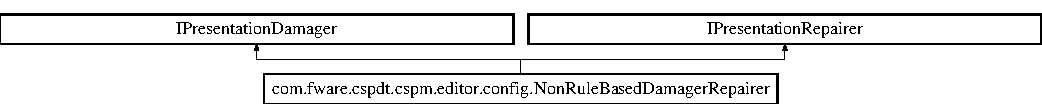
\includegraphics[height=1.372549cm]{classcom_1_1fware_1_1cspdt_1_1cspm_1_1editor_1_1config_1_1_non_rule_based_damager_repairer}
\end{center}
\end{figure}
\subsection*{Public Member Functions}
\begin{DoxyCompactItemize}
\item 
\mbox{\Hypertarget{classcom_1_1fware_1_1cspdt_1_1cspm_1_1editor_1_1config_1_1_non_rule_based_damager_repairer_af36e6a07ac9c5ed46856284f25b72811}\label{classcom_1_1fware_1_1cspdt_1_1cspm_1_1editor_1_1config_1_1_non_rule_based_damager_repairer_af36e6a07ac9c5ed46856284f25b72811}} 
\hyperlink{classcom_1_1fware_1_1cspdt_1_1cspm_1_1editor_1_1config_1_1_non_rule_based_damager_repairer_af36e6a07ac9c5ed46856284f25b72811}{Non\+Rule\+Based\+Damager\+Repairer} (Text\+Attribute default\+Text\+Attribute)
\begin{DoxyCompactList}\small\item\em Constructor for \hyperlink{classcom_1_1fware_1_1cspdt_1_1cspm_1_1editor_1_1config_1_1_non_rule_based_damager_repairer}{Non\+Rule\+Based\+Damager\+Repairer}. \end{DoxyCompactList}\item 
void \hyperlink{classcom_1_1fware_1_1cspdt_1_1cspm_1_1editor_1_1config_1_1_non_rule_based_damager_repairer_ae8015f432b2c8182cc3f981999a0874a}{set\+Document} (I\+Document document)
\item 
I\+Region \hyperlink{classcom_1_1fware_1_1cspdt_1_1cspm_1_1editor_1_1config_1_1_non_rule_based_damager_repairer_a6916df3bc6d3838ac23b4bdc7ab3799c}{get\+Damage\+Region} (I\+Typed\+Region partition, Document\+Event event, boolean document\+Partitioning\+Changed)
\item 
void \hyperlink{classcom_1_1fware_1_1cspdt_1_1cspm_1_1editor_1_1config_1_1_non_rule_based_damager_repairer_a502091b5e822b3d552cb1a3fad459d8b}{create\+Presentation} (Text\+Presentation presentation, I\+Typed\+Region region)
\end{DoxyCompactItemize}
\subsection*{Protected Member Functions}
\begin{DoxyCompactItemize}
\item 
int \hyperlink{classcom_1_1fware_1_1cspdt_1_1cspm_1_1editor_1_1config_1_1_non_rule_based_damager_repairer_a3e3084dfd0d0995dee91f6a2c23ee43e}{end\+Of\+Line\+Of} (int offset)  throws Bad\+Location\+Exception 
\begin{DoxyCompactList}\small\item\em Returns the end offset of the line that contains the specified offset or if the offset is inside a line delimiter, the end offset of the next line. \end{DoxyCompactList}\item 
void \hyperlink{classcom_1_1fware_1_1cspdt_1_1cspm_1_1editor_1_1config_1_1_non_rule_based_damager_repairer_a0fed10472da4fc71c06b37826c25b247}{add\+Range} (Text\+Presentation presentation, int offset, int length, Text\+Attribute attr)
\begin{DoxyCompactList}\small\item\em Adds style information to the given text presentation. \end{DoxyCompactList}\end{DoxyCompactItemize}
\subsection*{Protected Attributes}
\begin{DoxyCompactItemize}
\item 
\mbox{\Hypertarget{classcom_1_1fware_1_1cspdt_1_1cspm_1_1editor_1_1config_1_1_non_rule_based_damager_repairer_a295dc05aa1d1c74b90f2b23ebd345c59}\label{classcom_1_1fware_1_1cspdt_1_1cspm_1_1editor_1_1config_1_1_non_rule_based_damager_repairer_a295dc05aa1d1c74b90f2b23ebd345c59}} 
I\+Document \hyperlink{classcom_1_1fware_1_1cspdt_1_1cspm_1_1editor_1_1config_1_1_non_rule_based_damager_repairer_a295dc05aa1d1c74b90f2b23ebd345c59}{f\+Document}
\begin{DoxyCompactList}\small\item\em The document this object works on. \end{DoxyCompactList}\item 
\mbox{\Hypertarget{classcom_1_1fware_1_1cspdt_1_1cspm_1_1editor_1_1config_1_1_non_rule_based_damager_repairer_a259b7a776b8451c81d1ad57f536056c4}\label{classcom_1_1fware_1_1cspdt_1_1cspm_1_1editor_1_1config_1_1_non_rule_based_damager_repairer_a259b7a776b8451c81d1ad57f536056c4}} 
Text\+Attribute \hyperlink{classcom_1_1fware_1_1cspdt_1_1cspm_1_1editor_1_1config_1_1_non_rule_based_damager_repairer_a259b7a776b8451c81d1ad57f536056c4}{f\+Default\+Text\+Attribute}
\begin{DoxyCompactList}\small\item\em The default text attribute if non is returned as data by the current token. \end{DoxyCompactList}\end{DoxyCompactItemize}


\subsection{Detailed Description}
Esta classe e definida para aplicar a devida coloracao no texto sem precisar de regras. 

\begin{DoxyAuthor}{Author}
A\+L\+V\+A\+RO, E\+V\+E\+R\+A\+L\+DA, F\+E\+L\+I\+PE, J\+O\+N\+A\+T\+H\+AN, J\+U\+V\+E\+N\+AL 
\end{DoxyAuthor}


\subsection{Member Function Documentation}
\mbox{\Hypertarget{classcom_1_1fware_1_1cspdt_1_1cspm_1_1editor_1_1config_1_1_non_rule_based_damager_repairer_a0fed10472da4fc71c06b37826c25b247}\label{classcom_1_1fware_1_1cspdt_1_1cspm_1_1editor_1_1config_1_1_non_rule_based_damager_repairer_a0fed10472da4fc71c06b37826c25b247}} 
\index{com\+::fware\+::cspdt\+::cspm\+::editor\+::config\+::\+Non\+Rule\+Based\+Damager\+Repairer@{com\+::fware\+::cspdt\+::cspm\+::editor\+::config\+::\+Non\+Rule\+Based\+Damager\+Repairer}!add\+Range@{add\+Range}}
\index{add\+Range@{add\+Range}!com\+::fware\+::cspdt\+::cspm\+::editor\+::config\+::\+Non\+Rule\+Based\+Damager\+Repairer@{com\+::fware\+::cspdt\+::cspm\+::editor\+::config\+::\+Non\+Rule\+Based\+Damager\+Repairer}}
\subsubsection{\texorpdfstring{add\+Range()}{addRange()}}
{\footnotesize\ttfamily void com.\+fware.\+cspdt.\+cspm.\+editor.\+config.\+Non\+Rule\+Based\+Damager\+Repairer.\+add\+Range (\begin{DoxyParamCaption}\item[{Text\+Presentation}]{presentation,  }\item[{int}]{offset,  }\item[{int}]{length,  }\item[{Text\+Attribute}]{attr }\end{DoxyParamCaption})\hspace{0.3cm}{\ttfamily [inline]}, {\ttfamily [protected]}}



Adds style information to the given text presentation. 


\begin{DoxyParams}{Parameters}
{\em presentation} & the text presentation to be extended \\
\hline
{\em offset} & the offset of the range to be styled \\
\hline
{\em length} & the length of the range to be styled \\
\hline
{\em attr} & the attribute describing the style of the range to be styled \\
\hline
\end{DoxyParams}
\mbox{\Hypertarget{classcom_1_1fware_1_1cspdt_1_1cspm_1_1editor_1_1config_1_1_non_rule_based_damager_repairer_a502091b5e822b3d552cb1a3fad459d8b}\label{classcom_1_1fware_1_1cspdt_1_1cspm_1_1editor_1_1config_1_1_non_rule_based_damager_repairer_a502091b5e822b3d552cb1a3fad459d8b}} 
\index{com\+::fware\+::cspdt\+::cspm\+::editor\+::config\+::\+Non\+Rule\+Based\+Damager\+Repairer@{com\+::fware\+::cspdt\+::cspm\+::editor\+::config\+::\+Non\+Rule\+Based\+Damager\+Repairer}!create\+Presentation@{create\+Presentation}}
\index{create\+Presentation@{create\+Presentation}!com\+::fware\+::cspdt\+::cspm\+::editor\+::config\+::\+Non\+Rule\+Based\+Damager\+Repairer@{com\+::fware\+::cspdt\+::cspm\+::editor\+::config\+::\+Non\+Rule\+Based\+Damager\+Repairer}}
\subsubsection{\texorpdfstring{create\+Presentation()}{createPresentation()}}
{\footnotesize\ttfamily void com.\+fware.\+cspdt.\+cspm.\+editor.\+config.\+Non\+Rule\+Based\+Damager\+Repairer.\+create\+Presentation (\begin{DoxyParamCaption}\item[{Text\+Presentation}]{presentation,  }\item[{I\+Typed\+Region}]{region }\end{DoxyParamCaption})\hspace{0.3cm}{\ttfamily [inline]}}

\begin{DoxySeeAlso}{See also}
I\+Presentation\+Repairer\+::create\+Presentation(Text\+Presentation, I\+Typed\+Region) 
\end{DoxySeeAlso}
\mbox{\Hypertarget{classcom_1_1fware_1_1cspdt_1_1cspm_1_1editor_1_1config_1_1_non_rule_based_damager_repairer_a3e3084dfd0d0995dee91f6a2c23ee43e}\label{classcom_1_1fware_1_1cspdt_1_1cspm_1_1editor_1_1config_1_1_non_rule_based_damager_repairer_a3e3084dfd0d0995dee91f6a2c23ee43e}} 
\index{com\+::fware\+::cspdt\+::cspm\+::editor\+::config\+::\+Non\+Rule\+Based\+Damager\+Repairer@{com\+::fware\+::cspdt\+::cspm\+::editor\+::config\+::\+Non\+Rule\+Based\+Damager\+Repairer}!end\+Of\+Line\+Of@{end\+Of\+Line\+Of}}
\index{end\+Of\+Line\+Of@{end\+Of\+Line\+Of}!com\+::fware\+::cspdt\+::cspm\+::editor\+::config\+::\+Non\+Rule\+Based\+Damager\+Repairer@{com\+::fware\+::cspdt\+::cspm\+::editor\+::config\+::\+Non\+Rule\+Based\+Damager\+Repairer}}
\subsubsection{\texorpdfstring{end\+Of\+Line\+Of()}{endOfLineOf()}}
{\footnotesize\ttfamily int com.\+fware.\+cspdt.\+cspm.\+editor.\+config.\+Non\+Rule\+Based\+Damager\+Repairer.\+end\+Of\+Line\+Of (\begin{DoxyParamCaption}\item[{int}]{offset }\end{DoxyParamCaption}) throws Bad\+Location\+Exception\hspace{0.3cm}{\ttfamily [inline]}, {\ttfamily [protected]}}



Returns the end offset of the line that contains the specified offset or if the offset is inside a line delimiter, the end offset of the next line. 


\begin{DoxyParams}{Parameters}
{\em offset} & the offset whose line end offset must be computed \\
\hline
\end{DoxyParams}
\begin{DoxyReturn}{Returns}
the line end offset for the given offset 
\end{DoxyReturn}

\begin{DoxyExceptions}{Exceptions}
{\em Bad\+Location\+Exception} & if offset is invalid in the current document \\
\hline
\end{DoxyExceptions}
\mbox{\Hypertarget{classcom_1_1fware_1_1cspdt_1_1cspm_1_1editor_1_1config_1_1_non_rule_based_damager_repairer_a6916df3bc6d3838ac23b4bdc7ab3799c}\label{classcom_1_1fware_1_1cspdt_1_1cspm_1_1editor_1_1config_1_1_non_rule_based_damager_repairer_a6916df3bc6d3838ac23b4bdc7ab3799c}} 
\index{com\+::fware\+::cspdt\+::cspm\+::editor\+::config\+::\+Non\+Rule\+Based\+Damager\+Repairer@{com\+::fware\+::cspdt\+::cspm\+::editor\+::config\+::\+Non\+Rule\+Based\+Damager\+Repairer}!get\+Damage\+Region@{get\+Damage\+Region}}
\index{get\+Damage\+Region@{get\+Damage\+Region}!com\+::fware\+::cspdt\+::cspm\+::editor\+::config\+::\+Non\+Rule\+Based\+Damager\+Repairer@{com\+::fware\+::cspdt\+::cspm\+::editor\+::config\+::\+Non\+Rule\+Based\+Damager\+Repairer}}
\subsubsection{\texorpdfstring{get\+Damage\+Region()}{getDamageRegion()}}
{\footnotesize\ttfamily I\+Region com.\+fware.\+cspdt.\+cspm.\+editor.\+config.\+Non\+Rule\+Based\+Damager\+Repairer.\+get\+Damage\+Region (\begin{DoxyParamCaption}\item[{I\+Typed\+Region}]{partition,  }\item[{Document\+Event}]{event,  }\item[{boolean}]{document\+Partitioning\+Changed }\end{DoxyParamCaption})\hspace{0.3cm}{\ttfamily [inline]}}

\begin{DoxySeeAlso}{See also}
I\+Presentation\+Damager\+::get\+Damage\+Region(I\+Typed\+Region, Document\+Event, boolean) 
\end{DoxySeeAlso}
\mbox{\Hypertarget{classcom_1_1fware_1_1cspdt_1_1cspm_1_1editor_1_1config_1_1_non_rule_based_damager_repairer_ae8015f432b2c8182cc3f981999a0874a}\label{classcom_1_1fware_1_1cspdt_1_1cspm_1_1editor_1_1config_1_1_non_rule_based_damager_repairer_ae8015f432b2c8182cc3f981999a0874a}} 
\index{com\+::fware\+::cspdt\+::cspm\+::editor\+::config\+::\+Non\+Rule\+Based\+Damager\+Repairer@{com\+::fware\+::cspdt\+::cspm\+::editor\+::config\+::\+Non\+Rule\+Based\+Damager\+Repairer}!set\+Document@{set\+Document}}
\index{set\+Document@{set\+Document}!com\+::fware\+::cspdt\+::cspm\+::editor\+::config\+::\+Non\+Rule\+Based\+Damager\+Repairer@{com\+::fware\+::cspdt\+::cspm\+::editor\+::config\+::\+Non\+Rule\+Based\+Damager\+Repairer}}
\subsubsection{\texorpdfstring{set\+Document()}{setDocument()}}
{\footnotesize\ttfamily void com.\+fware.\+cspdt.\+cspm.\+editor.\+config.\+Non\+Rule\+Based\+Damager\+Repairer.\+set\+Document (\begin{DoxyParamCaption}\item[{I\+Document}]{document }\end{DoxyParamCaption})\hspace{0.3cm}{\ttfamily [inline]}}

\begin{DoxySeeAlso}{See also}
I\+Presentation\+Repairer\+::set\+Document(\+I\+Document) 
\end{DoxySeeAlso}


The documentation for this class was generated from the following file\+:\begin{DoxyCompactItemize}
\item 
C\+:/\+Users/\+E\+V\+A/\+Downloads/eclipse/workspace/cspdt/com.\+fware.\+cspdt.\+cspm.\+editor/src/com/fware/cspdt/cspm/editor/config/Non\+Rule\+Based\+Damager\+Repairer.\+java\end{DoxyCompactItemize}

\hypertarget{classcom_1_1fware_1_1cspdt_1_1cspm_1_1editor_1_1partition_1_1_process_rule}{}\section{com.\+fware.\+cspdt.\+cspm.\+editor.\+partition.\+Process\+Rule Class Reference}
\label{classcom_1_1fware_1_1cspdt_1_1cspm_1_1editor_1_1partition_1_1_process_rule}\index{com.\+fware.\+cspdt.\+cspm.\+editor.\+partition.\+Process\+Rule@{com.\+fware.\+cspdt.\+cspm.\+editor.\+partition.\+Process\+Rule}}
Inheritance diagram for com.\+fware.\+cspdt.\+cspm.\+editor.\+partition.\+Process\+Rule\+:\begin{figure}[H]
\begin{center}
\leavevmode
\includegraphics[height=2.000000cm]{classcom_1_1fware_1_1cspdt_1_1cspm_1_1editor_1_1partition_1_1_process_rule}
\end{center}
\end{figure}
\subsection*{Public Member Functions}
\begin{DoxyCompactItemize}
\item 
\mbox{\Hypertarget{classcom_1_1fware_1_1cspdt_1_1cspm_1_1editor_1_1partition_1_1_process_rule_a2821571086365f56f950f27d7a4b610d}\label{classcom_1_1fware_1_1cspdt_1_1cspm_1_1editor_1_1partition_1_1_process_rule_a2821571086365f56f950f27d7a4b610d}} 
{\bfseries Process\+Rule} (I\+Token process\+Token)
\item 
\mbox{\Hypertarget{classcom_1_1fware_1_1cspdt_1_1cspm_1_1editor_1_1partition_1_1_process_rule_a2a6f03e0864e834bed4c8f69df0e7381}\label{classcom_1_1fware_1_1cspdt_1_1cspm_1_1editor_1_1partition_1_1_process_rule_a2a6f03e0864e834bed4c8f69df0e7381}} 
I\+Token {\bfseries evaluate} (I\+Character\+Scanner scanner)
\item 
\mbox{\Hypertarget{classcom_1_1fware_1_1cspdt_1_1cspm_1_1editor_1_1partition_1_1_process_rule_a27b705bd337d8a3261ae7e92a59e5e89}\label{classcom_1_1fware_1_1cspdt_1_1cspm_1_1editor_1_1partition_1_1_process_rule_a27b705bd337d8a3261ae7e92a59e5e89}} 
I\+Token {\bfseries get\+Success\+Token} ()
\item 
\mbox{\Hypertarget{classcom_1_1fware_1_1cspdt_1_1cspm_1_1editor_1_1partition_1_1_process_rule_a8124341b2f7ea0a281fbcb3cad2cf434}\label{classcom_1_1fware_1_1cspdt_1_1cspm_1_1editor_1_1partition_1_1_process_rule_a8124341b2f7ea0a281fbcb3cad2cf434}} 
I\+Token {\bfseries evaluate} (I\+Character\+Scanner scanner, boolean resume)
\end{DoxyCompactItemize}


The documentation for this class was generated from the following file\+:\begin{DoxyCompactItemize}
\item 
C\+:/\+Users/\+E\+V\+A/\+Downloads/eclipse/workspace/cspdt/com.\+fware.\+cspdt.\+cspm.\+editor/src/com/fware/cspdt/cspm/editor/partition/Process\+Rule.\+java\end{DoxyCompactItemize}

%--- End generated contents ---

% Index
\backmatter
\newpage
\phantomsection
\clearemptydoublepage
\addcontentsline{toc}{chapter}{Index}
\printindex

\end{document}
